% Options for packages loaded elsewhere
\PassOptionsToPackage{unicode}{hyperref}
\PassOptionsToPackage{hyphens}{url}
%
\documentclass[
  man]{apa6}
\usepackage{amsmath,amssymb}
\usepackage{iftex}
\ifPDFTeX
  \usepackage[T1]{fontenc}
  \usepackage[utf8]{inputenc}
  \usepackage{textcomp} % provide euro and other symbols
\else % if luatex or xetex
  \usepackage{unicode-math} % this also loads fontspec
  \defaultfontfeatures{Scale=MatchLowercase}
  \defaultfontfeatures[\rmfamily]{Ligatures=TeX,Scale=1}
\fi
\usepackage{lmodern}
\ifPDFTeX\else
  % xetex/luatex font selection
\fi
% Use upquote if available, for straight quotes in verbatim environments
\IfFileExists{upquote.sty}{\usepackage{upquote}}{}
\IfFileExists{microtype.sty}{% use microtype if available
  \usepackage[]{microtype}
  \UseMicrotypeSet[protrusion]{basicmath} % disable protrusion for tt fonts
}{}
\makeatletter
\@ifundefined{KOMAClassName}{% if non-KOMA class
  \IfFileExists{parskip.sty}{%
    \usepackage{parskip}
  }{% else
    \setlength{\parindent}{0pt}
    \setlength{\parskip}{6pt plus 2pt minus 1pt}}
}{% if KOMA class
  \KOMAoptions{parskip=half}}
\makeatother
\usepackage{xcolor}
\usepackage{graphicx}
\makeatletter
\def\maxwidth{\ifdim\Gin@nat@width>\linewidth\linewidth\else\Gin@nat@width\fi}
\def\maxheight{\ifdim\Gin@nat@height>\textheight\textheight\else\Gin@nat@height\fi}
\makeatother
% Scale images if necessary, so that they will not overflow the page
% margins by default, and it is still possible to overwrite the defaults
% using explicit options in \includegraphics[width, height, ...]{}
\setkeys{Gin}{width=\maxwidth,height=\maxheight,keepaspectratio}
% Set default figure placement to htbp
\makeatletter
\def\fps@figure{htbp}
\makeatother
\setlength{\emergencystretch}{3em} % prevent overfull lines
\providecommand{\tightlist}{%
  \setlength{\itemsep}{0pt}\setlength{\parskip}{0pt}}
\setcounter{secnumdepth}{-\maxdimen} % remove section numbering
% Make \paragraph and \subparagraph free-standing
\makeatletter
\ifx\paragraph\undefined\else
  \let\oldparagraph\paragraph
  \renewcommand{\paragraph}{
    \@ifstar
      \xxxParagraphStar
      \xxxParagraphNoStar
  }
  \newcommand{\xxxParagraphStar}[1]{\oldparagraph*{#1}\mbox{}}
  \newcommand{\xxxParagraphNoStar}[1]{\oldparagraph{#1}\mbox{}}
\fi
\ifx\subparagraph\undefined\else
  \let\oldsubparagraph\subparagraph
  \renewcommand{\subparagraph}{
    \@ifstar
      \xxxSubParagraphStar
      \xxxSubParagraphNoStar
  }
  \newcommand{\xxxSubParagraphStar}[1]{\oldsubparagraph*{#1}\mbox{}}
  \newcommand{\xxxSubParagraphNoStar}[1]{\oldsubparagraph{#1}\mbox{}}
\fi
\makeatother
% definitions for citeproc citations
\NewDocumentCommand\citeproctext{}{}
\NewDocumentCommand\citeproc{mm}{%
  \begingroup\def\citeproctext{#2}\cite{#1}\endgroup}
\makeatletter
 % allow citations to break across lines
 \let\@cite@ofmt\@firstofone
 % avoid brackets around text for \cite:
 \def\@biblabel#1{}
 \def\@cite#1#2{{#1\if@tempswa , #2\fi}}
\makeatother
\newlength{\cslhangindent}
\setlength{\cslhangindent}{1.5em}
\newlength{\csllabelwidth}
\setlength{\csllabelwidth}{3em}
\newenvironment{CSLReferences}[2] % #1 hanging-indent, #2 entry-spacing
 {\begin{list}{}{%
  \setlength{\itemindent}{0pt}
  \setlength{\leftmargin}{0pt}
  \setlength{\parsep}{0pt}
  % turn on hanging indent if param 1 is 1
  \ifodd #1
   \setlength{\leftmargin}{\cslhangindent}
   \setlength{\itemindent}{-1\cslhangindent}
  \fi
  % set entry spacing
  \setlength{\itemsep}{#2\baselineskip}}}
 {\end{list}}
\usepackage{calc}
\newcommand{\CSLBlock}[1]{\hfill\break\parbox[t]{\linewidth}{\strut\ignorespaces#1\strut}}
\newcommand{\CSLLeftMargin}[1]{\parbox[t]{\csllabelwidth}{\strut#1\strut}}
\newcommand{\CSLRightInline}[1]{\parbox[t]{\linewidth - \csllabelwidth}{\strut#1\strut}}
\newcommand{\CSLIndent}[1]{\hspace{\cslhangindent}#1}
\ifLuaTeX
\usepackage[bidi=basic]{babel}
\else
\usepackage[bidi=default]{babel}
\fi
\babelprovide[main,import]{english}
% get rid of language-specific shorthands (see #6817):
\let\LanguageShortHands\languageshorthands
\def\languageshorthands#1{}
% Manuscript styling
\usepackage{upgreek}
\captionsetup{font=singlespacing,justification=justified}

% Table formatting
\usepackage{longtable}
\usepackage{lscape}
% \usepackage[counterclockwise]{rotating}   % Landscape page setup for large tables
\usepackage{multirow}		% Table styling
\usepackage{tabularx}		% Control Column width
\usepackage[flushleft]{threeparttable}	% Allows for three part tables with a specified notes section
\usepackage{threeparttablex}            % Lets threeparttable work with longtable

% Create new environments so endfloat can handle them
% \newenvironment{ltable}
%   {\begin{landscape}\centering\begin{threeparttable}}
%   {\end{threeparttable}\end{landscape}}
\newenvironment{lltable}{\begin{landscape}\centering\begin{ThreePartTable}}{\end{ThreePartTable}\end{landscape}}

% Enables adjusting longtable caption width to table width
% Solution found at http://golatex.de/longtable-mit-caption-so-breit-wie-die-tabelle-t15767.html
\makeatletter
\newcommand\LastLTentrywidth{1em}
\newlength\longtablewidth
\setlength{\longtablewidth}{1in}
\newcommand{\getlongtablewidth}{\begingroup \ifcsname LT@\roman{LT@tables}\endcsname \global\longtablewidth=0pt \renewcommand{\LT@entry}[2]{\global\advance\longtablewidth by ##2\relax\gdef\LastLTentrywidth{##2}}\@nameuse{LT@\roman{LT@tables}} \fi \endgroup}

% \setlength{\parindent}{0.5in}
% \setlength{\parskip}{0pt plus 0pt minus 0pt}

% Overwrite redefinition of paragraph and subparagraph by the default LaTeX template
% See https://github.com/crsh/papaja/issues/292
\makeatletter
\renewcommand{\paragraph}{\@startsection{paragraph}{4}{\parindent}%
  {0\baselineskip \@plus 0.2ex \@minus 0.2ex}%
  {-1em}%
  {\normalfont\normalsize\bfseries\itshape\typesectitle}}

\renewcommand{\subparagraph}[1]{\@startsection{subparagraph}{5}{1em}%
  {0\baselineskip \@plus 0.2ex \@minus 0.2ex}%
  {-\z@\relax}%
  {\normalfont\normalsize\itshape\hspace{\parindent}{#1}\textit{\addperi}}{\relax}}
\makeatother

\makeatletter
\usepackage{etoolbox}
\patchcmd{\maketitle}
  {\section{\normalfont\normalsize\abstractname}}
  {\section*{\normalfont\normalsize\abstractname}}
  {}{\typeout{Failed to patch abstract.}}
\patchcmd{\maketitle}
  {\section{\protect\normalfont{\@title}}}
  {\section*{\protect\normalfont{\@title}}}
  {}{\typeout{Failed to patch title.}}
\makeatother

\usepackage{xpatch}
\makeatletter
\xapptocmd\appendix
  {\xapptocmd\section
    {\addcontentsline{toc}{section}{\appendixname\ifoneappendix\else~\theappendix\fi\\: #1}}
    {}{\InnerPatchFailed}%
  }
{}{\PatchFailed}
\keywords{Misinformation; fake news; false news; news judgment; news accuracy; news discernment}
\DeclareDelayedFloatFlavor{ThreePartTable}{table}
\DeclareDelayedFloatFlavor{lltable}{table}
\DeclareDelayedFloatFlavor*{longtable}{table}
\makeatletter
\renewcommand{\efloat@iwrite}[1]{\immediate\expandafter\protected@write\csname efloat@post#1\endcsname{}}
\makeatother
\usepackage{csquotes}
\usepackage[titles]{tocloft}
\cftpagenumbersoff{figure}
\renewcommand{\cftfigpresnum}{\itshape\figurename\enspace}
\renewcommand{\cftfigaftersnum}{.\space}
\setlength{\cftfigindent}{0pt}
\setlength{\cftafterloftitleskip}{0pt}
\settowidth{\cftfignumwidth}{Figure 10.\qquad}
\cftpagenumbersoff{table}
\renewcommand{\cfttabpresnum}{\itshape\tablename\enspace}
\renewcommand{\cfttabaftersnum}{.\space}
\setlength{\cfttabindent}{0pt}
\setlength{\cftafterloftitleskip}{0pt}
\settowidth{\cfttabnumwidth}{Table 10.\qquad}
\usepackage{placeins} 

\ifLuaTeX
  \usepackage{selnolig}  % disable illegal ligatures
\fi
\usepackage{bookmark}
\IfFileExists{xurl.sty}{\usepackage{xurl}}{} % add URL line breaks if available
\urlstyle{same}
\hypersetup{
  pdftitle={Spotting False News and Doubting True News, A Meta-Analysis of News Judgments},
  pdfauthor={Jan Pfänder1 \& Sacha Altay2},
  pdflang={en-EN},
  pdfkeywords={Misinformation; fake news; false news; news judgment; news accuracy; news discernment},
  hidelinks,
  pdfcreator={LaTeX via pandoc}}

\title{Spotting False News and Doubting True News, A Meta-Analysis of News Judgments}
\author{Jan Pfänder\textsuperscript{1} \& Sacha Altay\textsuperscript{2}}
\date{}


\shorttitle{A Meta-Analysis of News Judgment}

\authornote{

Correspondence concerning this article should be addressed to Sacha Altay. E-mail: \href{mailto:sacha.altay@gmail.com}{\nolinkurl{sacha.altay@gmail.com}}

}

\affiliation{\vspace{0.5cm}\textsuperscript{1} Institut Jean Nicod, Département d'études cognitives, ENS, EHESS, PSL University, CNRS, France\\\textsuperscript{2} Department of Political Science, University of Zurich, Switzerland}

\abstract{%
How good are people at judging the veracity of news? We conducted a systematic literature review and pre-registered meta-analysis of 303 effect sizes from 67 experimental articles evaluating accuracy ratings of true and fact-checked false news (\(N_{participants}\) = 194'438 from 40 countries across 7 continents). We found that people rated true news as more accurate than false news (Cohen's d = 1.12 {[}1.01, 1.22{]}, p \textless{} .001) and were better at rating false news as false than at rating true news as true (Cohen's d = 0.32 {[}0.24, 0.39{]}, p \textless{} .001). In other words, participants were able to discern true from false news, and erred on the side of skepticism rather than credulity. We found no evidence that the political concordance of the news had an effect on discernment, but participants were more skeptical of politically discordant news (Cohen's d = 0.78 {[}0.62, 0.94{]}, p \textless{} .001). These findings lend support to crowdsourced fact-checking initiatives, and suggest that, to improve discernment, there is more room to increase the acceptance of true news than to reduce the acceptance of fact-checked false news.
}



\begin{document}
\maketitle

\clearpage

\section{Main text}\label{main-text}

Many have expressed concerns that we live in a ``post-truth'' era and that people cannot tell the truth from falsehoods anymore. In parallel, populist leaders around the world have tried to erode trust in the news by delegitimizing journalists and the news media more broadly\textsuperscript{1}. Since the 2016 US presidential election, our systematic literature review shows that over 4000 scientific articles have been published on the topic of false news. Across the world, numerous experiments evaluating the effect of interventions against misinformation or susceptibility to misinformation have relied on a similar design feature: having participants rate the accuracy of true and fact-checked false headlines--typically in a Facebook-like format, with an image, title, lede, and source, or as an isolated title/claim. Taken together, these studies allow us to shed some light on the most common fears voiced about false news, namely that people may fall for false news, distrust true news, or may be unable to discern between true and false news. In particular, we investigated whether people rate true news as more accurate than fact-checked false news (discernment) and whether they were better at rating false news as inaccurate than at rating true news as accurate (skepticism bias). We also investigated various moderators of discernment and skepticism bias such as political congruence, the topic of the news, or the presence of a source.

Establishing whether people can spot false news is important to design interventions against misinformation: if people lack the skills to spot false news, interventions should be targeted at improving skills to detect false news, whereas if people have the ability to spot false news but nonetheless engage with it, the problem lies elsewhere and may be one of motivation or (in)attention that educational interventions may struggle to address.

Past work has reliably shown that people do not fare better than chance at detecting lies because most verbal and non-verbal cues people use to detect lies are unreliable\textsuperscript{2}. Why would this be any different for detecting false news? People make snap judgments to evaluate the quality of the news they come across\textsuperscript{3}, and rely on seemingly imperfect proxies such as the source of information, police and fonts, the presence of hyperlinks, the quality of visuals, ads, or the tone of the text\textsuperscript{4,5}. In experimental settings, participants report relying on intuitions and tacit knowledge to judge the accuracy of news headlines\textsuperscript{6}. Yet, a scoping review of the literature on belief in false news (including a total of 26 articles) has shown that, in experiments, participants ``can detect deceitful messages reasonably well''\textsuperscript{7}. Similarly, a survey on 150 misinformation experts has shown that 53\% of experts agree that ``people can tell the truth from falsehoods'' -- while only 25\% of experts disagreed with the statement\textsuperscript{6}. Unlike the unreliable proxies people rely on to detect lies in interpersonal contexts, there are reasons to believe that some of the cues people use to detect false news may, on average, be reliable. For instance, the news outlets people trust the least do publish lower quality news and more false news, as people's trust ratings of news outlets correlate strongly with fact-checkers ratings in the US and Europe\textsuperscript{8,9}. Moreover, false news has some distinctive properties, such as being more politically slanted\textsuperscript{10}, being more novel, surprising, or disgusting, being more sensationalist, funnier, less boring, and less negative\textsuperscript{11,12}, or being more interesting-if-true\textsuperscript{13}. These features aim at increasing engagement, but they do so at the expense of accuracy, and in many cases, people may pick up on it. This led us to pre-register the hypothesis that people would rate true news as more accurate than false news. Yet, legitimate concerns have been raised about the lack of data outside of the US, especially in some Global South countries where the misinformation problem is arguably worse. Our meta-analysis covers 40 countries across 7 continents and directly addresses concerns about the over-representation of US-data.

\textbf{H1: People rate true news as more accurate than false news.}

While many fear that people are exposed to too much misinformation, too easily fall for it, and are overly influenced by it, a growing body of researchers is worried that people are exposed to too little reliable information, commonly reject it, and are excessively resistant to it\textsuperscript{14,15}. Establishing whether true news skepticism (excessively rejecting true news) is of similar magnitude to false news gullibility (excessively accepting false news) is important for future studies on misinformation: if people are excessively gullible, interventions should primarily aim at fostering skepticism, whereas if people are excessively skeptical, interventions should focus on increasing trust in reliable information. For these reasons, in addition to investigating discernment (H1), we also looked at skepticism bias by comparing the magnitude of true news skepticism to false news gullibility. Research in psychology has shown that people exhibit a ``truth bias''\textsuperscript{16,17}, such that they tend to accept incoming statements rather than reject them. Similarly, work on interpersonal communication has shown that, by default, people tend to accept communicated information\textsuperscript{18}. However, there are reasons to think that the truth-default-theory may not apply to news judgments. It has been hypothesized that people display a truth bias in interpersonal contexts because information in these contexts is, in fact, often true\textsuperscript{16}. When it comes to news judgments, it is not clear that people by default expect news stories to be true. Trust in the news and journalists is low worldwide\textsuperscript{19}, and a significant part of the population holds cynical views of the news\textsuperscript{20}. Similarly, populist leaders across the world have attacked the credibility of the news media and instrumentalized the concept of fake news to discredit quality journalism\textsuperscript{21,22}. Disinformation strategies such as ``flooding the zone'' with false information\textsuperscript{23,24} have been shown to increase skepticism in news judgments\textsuperscript{6}. Moreover, in many studies included in our meta-analysis, the news stories were presented in a social media format (most often Facebook), which could fuel skepticism in news judgments. Indeed, people trust news\textsuperscript{3} and information more generally\textsuperscript{25} less on social media than on news websites. In line with these observations, some empirical evidence suggests that for news judgments, people display the opposite of a truth bias\textsuperscript{26}, namely a conservative skepticism bias, whereby people tend to rate all news as more false than they are\textsuperscript{6,27,28}. We thus predicted that when judging the accuracy of news, participants will err on the side of skepticism more than on the side of gullibility. Precisely, we predicted that people will be better at rating false news as false than rating true news as true.

\textbf{H2: People are better at rating false news as false than true news as true.}

Finally, we investigated potential moderators of H1 and H2, such as the country where the experiment was conducted, the format of the news headlines, the topic, whether the source of the news was displayed, and political concordance of the news. Past work has suggested that displaying the source of the news has a small effect at best on accuracy ratings\textsuperscript{29}, whereas little work has investigated differences in news judgments across countries, topics, and formats. The effect of political concordance on news judgments is debated. Participants may be motivated to believe politically congruent (true and false) news, motivated to disbelieve politically incongruent news, or not be politically motivated at all but still display such biases\textsuperscript{30}. We formulated research questions instead of hypotheses for our moderator analyses because of a lack of strong theoretical expectations.

\subsection{The present study}\label{the-present-study}

We conducted a systematic literature review and pre-registered meta-analysis based on 67 publications, providing data on 195 samples (194438 participants) and 303 effects (i.e.~\textbf{k}, the meta-analytic observations). Sometimes, a sample provided several effect sizes, for example when separate accuracy ratings are available by news topic, or when follow-up studies were conducted on the same participants. A common case where a sample provides several effect sizes is when participants rated both politically concordant and discordant news. In this case, if possible, we entered summary statistics separately for the concordant and discordant items, yielding two effect sizes (i.e.~two different rows in our data frame). We account for the resulting hierarchical structure of the data in our statistical models. For a publication to be included in our meta-analysis, we set six eligibility criteria: (1) We considered as relevant all document types with original data (not only published ones, but also reports, pre-prints and working papers). When different publications were using the same data, a scenario we encountered several times, we included only one publication (which we picked arbitrarily). (2) We only included articles that measured perceived accuracy (including ``accuracy'', ``credibility'', ``trustworthiness'', ``reliability'' or ``manipulativeness''), and (3) did so for both true and false news. (4) We only included studies relying on real-world news items. Accordingly, we excluded studies in which researchers made up the false news items, or manipulated the properties of the true news items. (5) We could only include articles that provided us with the relevant summary statistics (means and standard deviations for both false and true news), or publicly available data that allowed us to calculate those. In cases where we were not able to retrieve the relevant summary statistics either way, we contacted the authors. (6) Finally, to ensure comparability, we only included studies that provided a neutral control condition. For example,\textsuperscript{31}, among other things, test the effect of an interest prime vs.~an accuracy prime. A neutral control condition - one that is comparable to those of other studies - would have been no prime at all. We therefore excluded the paper. After starting the literature search, we added further search criteria in order to diminish the vast number of results (see \hyperref[methods]{methods}). Rejection decisions for all retrieved papers are documented and can be accessed on the \href{https://osf.io/96zbp/?view_only=d2f3147f652e44e2a0414d7d6d9a6c29}{OSF project page}. We provide a list of all included articles in Appendix \ref{included-studies}.

We found that, on average, people are good at discerning true from fact-checked false news, and rate true news as much more accurate than false news. However, they are slightly better at rating fact-checked false news as inaccurate than at rating true news as accurate.

\section{Results}\label{results}

\subsection{Descriptives}\label{descriptives}

Our meta-analysis includes publications from 40 countries across 7 continents. However, 34\% of all participants were recruited in the United States alone, and 53\% in Europe. Only 6\% of participants were recruited in Asia, and even less in Africa (2\%; see Fig. \ref{fig:map} for the number of effect sizes per country). The average sample size was 997.12 (min = 19, max = 32134, median = 482).

In total, participants rated the accuracy of 2167 unique news items. On average, a participant rated 19.76 news items per study (min = 2, max = 240, median = 18). For 71 samples, news items were sampled from a pool of news (the pool size ranged from 12 to 255, with an average pool size of 57.46 items). The vast majority of studies (294 out of 303 effects) used a within participant design for manipulating news veracity, with each participant rating both true and false news items. Almost all effect sizes are from online studies (286 out of 294).



\begin{figure}
\centering
\includegraphics{output/figures/map.pdf}
\caption{\label{fig:map}A map of the number of effect sizes per country.}
\end{figure}

\subsection{Analytic procedures}\label{analytic-procedures}

All analyses were pre-registered unless explicitly stated otherwise (for deviations see methods section). The choice of models was informed by simulations we conducted before having the data. To test H1, we calculated a discernment score by subtracting the mean accuracy ratings of false news from the mean accuracy ratings of true news, such that higher scores indicate better discernment. This differential measure of discernment is common in the literature on misinformation\textsuperscript{32}. To test H2, we first calculated a judgment error for true and false news respectively. Error is defined as the distance between optimal accuracy ratings and actual accuracy ratings. For false news, optimal ratings represent the bottom of the accuracy scale (see Fig. \ref{fig:descriptive}). False news error is thus computed as the distance between the accuracy score and the bottom of the scale. For instance, for an average false news accuracy rating of 2.2 on a 4-point accuracy scale going from 1, not accurate at all, to 4, completely accurate, the error would be: 2.2 - 1 = 1.2. For true news, optimal ratings represent the top of the accuracy scale (see Fig. \ref{fig:descriptive}). True news error is thus computed as the distance between the accuracy score and the top of the scale. For instance, for an average true news accuracy rating of 2.5 on a 4-point accuracy scale, the error would be: 4 - 2.5 = 1.5. We then calculate the skepticism bias as the difference between the two errors, subtracting the true news error score from the false news error score (e.g.~skepticism bias: 1.5 - 1.2 = 0.3). Note that we cannot use more established measures of discernment or response bias, such as Signal Detection Theory, because we rely on mean ratings and not individual ratings. However, in Appendix \ref{signal-detection-theory}, we show that for the studies we have raw data on, our main findings hold when relying on d' (sensitivity) and c (response bias) in Signal Detection Theory.

Fig. \ref{fig:descriptive} offers a descriptive (irrespective of sample sizes) overview of all accuracy ratings that we calculated our effect sizes from. On average, true news were rated as more accurate than false news, as shown by the positive discernment score (0.24). We also see that false news discrimination is better than true news discrimination, i.e., the distance between true news ratings and the top of the scale (0.40) is greater than the distance between false news ratings and bottom of the scale (0.36), yielding a positive skepticism bias (0.40 - 0.36 = 0.04).



\begin{figure}
\centering
\includegraphics{output/figures/descriptive.pdf}
\caption{\label{fig:descriptive}\emph{Illustration of outcome measures}. The figure shows the distributions of accuracy ratings for true and fact-checked false news, scaled to range from 0 to 1. The figure illustrates discernment (the distance between the mean for true news and the mean for false news) and the errors (distance to the right end for true news and to the left end for false news) from which the skepticism bias is computed. A larger error for true news compared to false news yields a positive skepticism bias. In this descriptive figure, unlike in the meta-analysis, ratings and effect sizes are not weighted by sample size.}
\end{figure}

Skepticism bias can only be (meaningfully) computed on scales using symmetrical labels, i.e.~the intensity of the labels to qualify true and false news are equivalent (e.g., ``True'' vs ``False'' or ``Definitely fake'' {[}1{]} to ``Definitely real'' {[}7{]}). 69\% of effects included in the meta-analysis used scales with perfectly symmetrical labels, while 26\% used imperfectly symmetrical scale labels, i.e., the intensity of the labels to qualify true and false news are similar but not equivalent (e.g., {[}1{]} not at all accurate, {[}2{]} not very accurate, {[}3{]} somewhat accurate, {[}4{]} very accurate; here for instance `not all accurate' is stronger than `very accurate'). Note that we could only compute this variable for scales that explicitly labeled each scale point, resulting in missing values for 5\% of effects. In Appendix \ref{moderators}, we show that scale symmetry has no statistically significant effect on skepticism bias.

To be able to compare effect sizes across different scales, we calculated Cohen's d, a common standardized mean difference. To account for statistical dependence between true and false news ratings arising from the within-participant design used by most studies (294 out of 303 effect sizes), we calculated the standard error following the \href{https://training.cochrane.org/handbook/current/chapter-23\#section-23-2-7-3}{Cochrane recommendations for crossover trials}\textsuperscript{33}. For the remaining 9 effect sizes from studies that used a between-participant design, we calculated the standard error assuming independence between true and false news ratings (see \hyperref[methods]{methods}). In Appendix \ref{effect-sizes}, we show that our results hold across alternative standardized effect measures, among which the one we had originally pre-registered, a standardized mean change using change score standardization (SMCC). We chose to deviate from the pre-registration and use Cohen's d instead, because it is easier to interpret and corresponds to the standards \href{https://training.cochrane.org/handbook/current/chapter-23\#section-23-2-7-3}{for crossover trials recommended by the Cochrane manual}\textsuperscript{33}. In Appendix \ref{effect-sizes}, we also provide effect estimates in units of the original scales separately for each scale.

We used multilevel meta models with clustered standard errors at the sample level to account for cases in which the same sample contributed various effect sizes (i.e.~the meta-analytic units of observation). All confidence intervals reported in this paper are 95\% confidence intervals. All statistical tests are two-tailed.

\subsection{Main results}\label{main-results}

\subsubsection{Discernment (H1)}\label{discernment-h1}



\begin{figure}
\centering
\includegraphics{output/figures/forest.pdf}
\caption{\label{fig:forest}\emph{Forest plots for discernment and skepticism bias}. The figure displays all n = 303 effect sizes for both outcomes. Effects are weighed by their sample size. Effect sizes are calculated as Cohen's d.~Horizontal bars represent 95\% confidence intervals. The average estimate is the result of a multilevel meta model with clustered standard errors at the sample level.}
\end{figure}

Supporting H1, participants rated true news as more accurate than false news on average. Pooled across all studies, the average discernment estimate is large (d = 1.12 {[}1.01, 1.22{]}, z = 20.79, p \textless{} .001). As shown in Fig. \ref{fig:forest}, 298 of 303 estimates are positive. Of the positive estimates, 3 have a confidence interval that includes 0, as does 1 of the negative estimates. Most of the variance in the effect sizes observed above is explained by between-sample heterogeneity (\(I2_{between}\) = 92.04\%). Within-sample heterogeneity is comparatively small (\(I2_{within}\) = 7.93\%), indicating that when the same participants were observed on several occasions (i.e.~the same sample contributed several effect sizes), on average, discernment performance was similar across those observations. The share of the variance attributed to sampling error is very small (0.03\%), which is indicative of the large sample sizes and thus precise estimates.

\subsubsection{Skepticism bias (H2)}\label{skepticism-bias-h2}

We found support for H2, with participants being better at rating false news as inaccurate than at rating true news as accurate (i.e.~false news discrimination was on average higher than true news discrimination). However, the average skepticism bias estimate is small (d = 0.32 {[}0.24, 0.39{]}, z = 8.11, p \textless{} .001). As shown in Fig \ref{fig:forest}, 203 of 303 estimates are positive. Of the positive estimates, 6 have a confidence interval that includes 0, as do 7 of the negative estimates. By contrast with discernment, most of the variance in skepticism bias is explained by within-sample heterogeneity (\(I2_{within}\) = 60.96\%; \(I2_{between}\) = 38.99\%; sampling error = 0.05\%). Whenever we observe within sample variation in our data, it is because several effects were available for the same sample. This is mostly the case for studies with multiple survey waves, or when effects were split by different news topics, suggesting that these factors may account for some of that variation. In the moderator analyses below, we compare across samples and broad categories, thereby glossing over much of that within variation for most variables.

\subsection{Moderators}\label{moderators}

Following the pre-registered analysis plan, we ran a separate meta regression for each moderator by adding the respective moderator variable as a fixed effect to the multilevel meta models. We report regression tables and visualizations in Appendix \ref{moderators}. Here, we report the regression coefficients as ``Delta''s, since they designate differences between categories. For example, in the moderator analysis of political concordance on skepticism bias, ``concordant'' marks the baseline category. The predicted value for this category can be read from the intercept (-.2). The ``Delta'' is the predicted difference between concordant and discordant (.78). To obtain the predicted value for discordant news, one needs to add the ``Delta'' to the intercept (-.2 + .78 = .58).

\paragraph{Cross-cultural variability}\label{cross-cultural-variability}

For samples based in the United States (184/303 effect sizes), discernment was higher than for samples based in other countries, on average (\(\Delta\) Discernment = 0.23 {[}0.02, 0.44{]}, z = 2.14 , p = 0.033 ; baseline discernment other countries pooled = 0.99 {[}0.84, 1.14{]}, z = 12.82, p \textless{} .001). However, we did not find a statistically significant difference regarding skepticism bias (\(\Delta\) Skepticism bias = 0.04 {[}-0.12, 0.19{]}, z = 0.47 , p = 0.638). A visualization of discernment (\ref{fig:discernment-countries}) and skepticism bias (\ref{fig:bias-countries}) across countries can be found in Appendix \ref{country-comparison}.

\paragraph{Scales}\label{scales}

The studies in our meta analysis used a variety of accuracy scales, including both binary (e.g.~``Do you think the above headline is accurate? - Yes, No'') and continuous ones (e.g.~``To the best of your knowledge, how accurate is the claim in the above headline'' 1 = Not at all accurate, 4 = Very accurate).

Regarding discernment, two scale types differed from the most common 4-point scale (Baseline discernment 4-point-scale = 1.28 {[}1.07, 1.49{]}, z = 11.96, p \textless{} .001): Both 6-point scales (\(\Delta\) Discernment = -0.41 {[}-0.7, -0.12{]}, z = -2.80, p = 0.006) and binary scales (\(\Delta\) Discernment = -0.37 {[}-0.66, -0.08{]}, z = -2.50, p = 0.013) yielded lower discernment. Regarding skepticism bias, studies using a 4-point scale (Baseline skepticism bias 4-point scale = 0.51 {[}0.3, 0.72{]}, z = 4.75, p \textless{} .001) reported a larger skepticism bias compared to studies using a binary and a 7-point scale (\(\Delta\) Skepticism bias = -0.29 {[}-0.51, -0.06{]}, z = -2.47, p = 0.014 for binary scales; -0.50 {[}-0.76, -0.23{]}, z = -3.67, p \textless{} .001 for 7-point scales). Interpreting the the observed differences is not straightforward. We attempt a more detailed discussion of differences between binary and Likert-scale studies in Appendix \ref{binary}.

\paragraph{Format}\label{format}

Studies using as stimuli headlines with pictures (\(\Delta\) Skepticism bias = 0.22 {[}0.04, 0.39{]}, z = 2.45, p = 0.015; 65 effects), or headlines with pictures and a lede (\(\Delta\) Skepticism bias = 0.33 {[}0.14, 0.52{]}, z = 3.40, p \textless{} .001; 56 effects), displayed a stronger skepticism bias compared to studies relying on headlines with no picture/lede (Baseline skepticism bias headlines only = 0.23 {[}0.13, 0.33{]}, z = 4.45, p \textless{} .001; 163 effects). We do not find differences related to format for discernment, neither for headlines with pictures (\(\Delta\) Discernment = -0.01 {[}-0.28, 0.27{]}, z = -0.04, p = 0.969), nor for headlines with pictures and a lede (\(\Delta\) Discernment = 0.11 {[}-0.12, 0.33{]}, z = 0.93, p = 0.353).

\paragraph{Topic}\label{topic}

We did not find statistically significant differences in discernment and skepticism bias across news topics, when distinguishing between the categories ``political'' (\(\Delta\) Skepticism bias = 0.03 {[}-0.13, 0.19{]}, z = 0.43, p = 0.671; \(\Delta\) Discernment = -0.26 {[}-0.51, 0{]}, z = -1.98, p = 0.049; 196 effects; 43 articles), ``covid'' (baseline; 54 effects; 13 articles) and ``other'' (\(\Delta\) Skepticism bias = -0.02 {[}-0.2, 0.16{]}, z = -0.22, p = 0.825; \(\Delta\) Discernment = -0.01 {[}-0.35, 0.34{]}, z = -0.03, p = 0.976; 53 effects; 20 articles), a category which regroups all not explicitly as ``covid''or ``political'' labeled news topics by the authors for the respective papers, and which includes news topics reaching from health, cancer and science, to economics, history and military covering news.

\paragraph{Sources}\label{sources}

In line with past findings, we did not observe a statistically significant difference in discernment between studies displaying the source of the news items (\(\Delta\) Discernment = -0.22 {[}-0.47, 0.03{]}, z = -1.75, p = 0.082; 112 effects) and studies that did not (147 effects; for 44 this information was not explicitly provided). We do not find a difference regarding skepticism bias either (\(\Delta\) Skepticism bias = 0.11 {[}-0.06, 0.29{]}, z = 1.30, p = 0.194).

\paragraph{Political Concordance}\label{political-concordance}

The moderators investigated above were (mostly) not experimentally manipulated within studies, but instead varied between studies, which impedes causal inference. Political concordance is an exception in this regard. It was manipulated within 31 different samples, across 14 different papers. In those experiments, typically, a pre-test establishes the political slant of news headlines (e.g.~pro-republican vs.~pro-democrat). In the main study, participants then rate the accuracy for news items of both political slants, and provide information about their own political stance. The ratings of items are then grouped into concordant or discordant (e.g.~pro-republican news rated by Republicans will be coded as concordant while pro-republican news rated by Democrats will be coded as discordant).

Political concordance had no statistically significant effect on discernment. However, participants displayed a skepticism bias only when rating politically discordant headlines (see Fig. \ref{fig:concordance}). In particular, when rating concordant items, there was no evidence that participants showed a skepticism bias (Baseline skepticism bias concordant items = -0.20 {[}-0.42, 0.01{]}, z = -1.93, p = 0.064), while for discordant news items, participants displayed a positive skepticism bias (\(\Delta\) Skepticism bias = 0.78 {[}0.62, 0.94{]}, z = 10.04, p \textless{} .001). In other words, participants were not gullible when facing concordant news headlines (as would have suggested a negative skepticism bias), but were skeptical when facing discordant ones.



\begin{figure}
\centering
\includegraphics{output/figures/concordance.pdf}
\caption{\label{fig:concordance}\emph{Effect of political concordance on discernment and skepticism bias}. The figure shows the distribution of the n = 44 effect sizes for politically concordant and discordant items. The black dots represent the predicted average of the meta-regression, the black horizontal bars the 95\% confidence intervals. Note that the figure does not represent the different weights (i.e.~the varying sample sizes) of the data points, but that these weights are taken into account in the meta-regression.}
\end{figure}

\subsection{Individual level data}\label{individual-level-data}

In the results above, accuracy ratings were averaged across participants. It is unclear how these average results generalize to the individual level. Do they hold for most participants? Or are they driven by a relatively small group of participants with excellent discernment skills, or, respectively, extreme skepticism? For 22 articles (\(N_{Participants}\) = 42074, \(N_{Observations}\) = 813517), we have the raw data for all ratings that individual participants made on each news headline they saw. On this data, we ran a descriptive, non-preregistered analysis: We calculated a discernment and skepticism bias score for each participant based on all the news items they were rating. To compare across different scales, we transposed all accuracy scores on a scale from 0 to 1, resulting in a range of possible values from -1 to 1 for both discernment and skepticism bias.



\begin{figure}
\centering
\includegraphics{output/figures/individual-level-plot.pdf}
\caption{\label{fig:individual-level-plot}\emph{Outcomes on the participant-level}. The figure shows the distribution of average discernment and skepticism bias scores of individual participants in the subset of studies that we have raw data on. We standardized original accuracy ratings to range from 0 to 1, to be able to compare across scales. Therefore, the worst possible score is -1 where, for discernment, an individual classified all news wrongly, and for skepticism bias, an individual classified all true news correctly (as true) and all false news incorrectly (as true). The best possible score is 1 where, for discernment, an individual classified all news correctly, and for skepticism bias, an individual classified all true news incorrectly (as false) and all false news correctly (as false). The percentage labels (from left to right) represent the share of participants with a negative score, a score of exactly 0, and a positive score, for both measures respectively.}
\end{figure}

As shown in Fig. \ref{fig:individual-level-plot}, 79.92 \% of individual participants had a positive discernment score, and 59.06 \% of participants had a positive skepticism bias score. Therefore, our main results based on mean ratings across participants seem to be representative of individual participants (see Appendix \ref{individual-level} for further discussion).

\section{Discussion}\label{discussion}

This meta-analysis sheds light on some of the most common fears voiced about false news. In particular, we investigated whether people are able to discern true from false news, and whether they are better at judging the veracity of true news or false news (skepticism bias). Across 303 effect sizes (\(N_{participants}\) = 194438) from 40 countries across 7 continents, we found that people rated true news as much more accurate than fact-checked false news (\(d_{discernment}\) = 1.12 {[}1.01, 1.22{]}, z = 20.79, p \textless{} .001) and are slightly better at rating fact-checked false news as inaccurate than at rating true news as accurate (\(d_{bias}\) = 0.32 {[}0.24, 0.39{]}, z = 8.11, p \textless{} .001).

The finding that people can discern true from false news when prompted to do so has important implications for interventions against misinformation. First, it suggests that most people do not lack the skills to spot false news -- at least the kind of fact-checked false news used in the studies included in our meta-analysis. If people don't lack the skills to spot false news, why do they sometimes fall for false news? In some contexts, people may lack the motivation to use their discernment skills or may only apply them selectively\textsuperscript{34,35}. Thus, instead of teaching people how to spot false news, it may be more fruitful to target motivations, either by manipulating features of the environment in which people encounter news\textsuperscript{36,37}, or by intrinsically motivating people to use their skills and pay more attention to accuracy\textsuperscript{34}. For instance, it has been shown that design features of current social media environments sometimes impede discernment\textsuperscript{38}. Similarly, it has been suggested that interventions against misinformation should build on the tacit knowledge that people (already) rely on to detect false news, instead of giving people explicit tips and guidelines that may be difficult for people to internalize as tacit knowledge\textsuperscript{39}.

Our results do not speak to the reasons why participants were able to discern true from false news. Participants were generally asked to rate culturally relevant news stories, such as Brazilians rating Brazilian news stories. Thus, participants most likely relied on some prior knowledge to evaluate news veracity. Participants would probably not have been capable of discerning news stories on which they completely lack relevant prior knowledge, e.g.~culturally distant news stories.

Second, the fact that people can, on average, discern true from false news lends support to crowdsourced fact-checking initiatives. While fact-checkers cannot keep up with the pace of false news production, the crowd can, and it has been shown that even small groups of participants perform as well as professional fact-checkers\textsuperscript{40,41}. The cross-cultural scope of our findings suggests that these initiatives may be fruitful in many countries across the world. In every country included in the meta-analysis, participants on average rated true news as more accurate than false news (see Appendix \ref{country-comparison}). Our results are also informative for the work of fact-checkers. In recent years, fact-checking organizations such as PolitiFact have mostly focused on debunking false news at the expense of confirming true news\textsuperscript{42}. Yet, we show that people also need help to identify true news as true. Moreover, since people are quite good at discerning true from false news, fact-checkers may want to focus on headlines that are less clearly false or true. However, we cannot rule out that people's current discerning skills stem in part from the work of fact-checkers.

The fact that people disbelieve true news slightly more than they believe fact-checked false news speaks to the nature of the misinformation problem and how to fight it: the problem may be less that people are gullible, and fall for falsehoods too easily, but instead that people are excessively skeptical, and do not believe reliable information enough\textsuperscript{15,43}. Even assuming that the rejection of true news and the acceptance of false news are of similar magnitude (and that both can be improved), given that true news are much more prevalent in people's news diet than false news\textsuperscript{44}, true news skepticism may be more detrimental to the accuracy of people's beliefs than false news acceptance\textsuperscript{14}. This skepticism is concerning in the context of the low and declining participation, trust and interest in news across the world\textsuperscript{45}, as well as the attacks of populist leaders on the news media\textsuperscript{22}, and growing news avoidance\textsuperscript{46}. Interventions aimed at reducing misperceptions should therefore consider increasing the acceptance of true news in addition to reducing the acceptance of false news\textsuperscript{14,47}. At the very least, when testing interventions, researchers should evaluate their effect on both true and false news, not just false news\textsuperscript{48}. At best, interventions should use methods that allow to estimate discrimination while accounting for response bias, such as Signal Detection Theory, and make sure that apparent increases in discernment are not due to more conservative response bias\textsuperscript{28,49}. This is all the more important given that recent evidence suggests that many interventions against misinformation, such as media literacy tips\textsuperscript{50}, fact-checking\textsuperscript{51}, or educational games aimed at inoculating people against misinformation\textsuperscript{28}, may reduce misperceptions of false news at the expense of true news.

The skepticism bias documented here may stem from the fact that it's easier for something to be false than for something to be true. Falsifying a statement is easier than confirming it: there only needs to be one black swan to falsify the statement that all swans are white whereas confirming this statement requires much more effort. This may explain why participants were more eager to classify news stories as false rather than true. Yet, it does not explain why the literature on interpersonal communication typically finds a truth bias and why people tend to show an acquiescence bias rather than a rejection bias\textsuperscript{16,52} .

We also investigated various moderators of discernment and skepticism bias. We found that discernment was greater in studies conducted in the United States compared to the rest of the world. This could be due to the inclusion of many countries from the Global South, where belief in misinformation and conspiracy theories has been documented to be higher\textsuperscript{53}. In line with past work\textsuperscript{29}, the presence of a source had no statistically significant effects. The topic of the news also had no statistically significant effects on discernment and skepticism bias. Participants showed greater skepticism (higher skepticism bias) in studies that presented headlines in a social media format (with an image and lede) or along with an image compared to studies that used plain headlines. This suggests that the skepticism of true news documented in this meta-analysis may be partially due to the social media format of the news headlines. Past work has shown that people report trusting news on social media less\textsuperscript{3,19}, and experimental manipulations have shown that the Facebook news format reduces belief in news\textsuperscript{54,55} --although the causal effects documented in these experiments are much smaller than observational differences in reported trust levels between news on social media and on news outlets\textsuperscript{56}. Low trust in news on social media may be a good thing, given that on average news on social media may be less accurate than news on news websites, but it is also worrying given that most of news consumption worldwide is shifting online and on social media in particular\textsuperscript{46}.

The political concordance of the news had no effect on discernment, but participants were excessively skeptical of politically discordant news. That is, participants were equally skilled at discerning true from false news for concordant and discordant items, but they rated news generally (true and false) as more false when politically discordant. This finding is in line with recent evidence on partisan biases in news judgments\textsuperscript{57}, and supports the idea that people are not excessively gullible of news they agree with, but are instead excessively skeptical of news they disagree with\textsuperscript{15,58}. It suggests that interventions aimed at reducing partisan motivated reasoning, or at improving political reasoning in general, should focus more on increasing openness to opposing viewpoints than on increasing skepticism towards concordant viewpoints. Future studies should investigate whether the effect of congruence is specific to politics or if it holds across topics, and compare it to a baseline by including neutral items.

Our meta-analysis has a number of conceptual limitations. First, participants evaluated the news stories in artificial settings that do not mimic the real-world. For instance, the mere fact of asking participants to rate the accuracy of the news stories may have increased discernment by increasing attention to accuracy\textsuperscript{34}. When browsing on social media, people may be less discerning (and perhaps less skeptical) than in experimental settings because they would pay less attention to accuracy\textsuperscript{38}. However, given people's low exposure to misinformation online\textsuperscript{59}, most people may protect themselves from misinformation not by detecting misinformation on the spot, but by relying on the reputation of the sources and avoiding unreliable sources\textsuperscript{60}. Second, accuracy ratings were averaged across participants and thus better reflect the wisdom of the crowd than the skills of individuals. Yet, past work\textsuperscript{40} shows that most individuals appear able to discern true from false news better than chance. In line with this, studies for which we have raw data show that 79.92 \% of participants rated true news as more accurate than false news, and 59.06 \% of participants displayed a skepticism bias (see Fig. \ref{fig:individual-level-plot}; see also Appendix \ref{individual-level} for additional analyses on individual-level data). Third, our results reflect choices made by researchers about news selection. As we lay out in Appendix \ref{selection-bias}, we believe that this selection bias mostly concerns the false news items. The vast majority of studies in our meta-analysis relied on fact-checked false news, determined by fact-checking websites (e.g.~Snopes, PolitiFact). By contrast, three papers\textsuperscript{40,61,62} automated their news selection by scraping headlines from media outlets in real-time, and had both participants and fact-checkers (or the researchers themselves, in the case of\textsuperscript{61}) rated the veracity of the headlies shortly after. The three studies (53 effect sizes; 10170 participants; all in the United States) find (i) lower discernment and (ii) a negative skepticism (i.e.~a credulity) bias. As we discuss in Appendix \ref{selection-bias}, this is likely because they included false news that are harder to fact-check (and not typically fact-checked) or because the news are less false than the typical fact-checked false news. Yet, more work is needed to investigate whether the skepticism bias documented here is due to the selection of fact-checked false news or to something else. This highlights the importance of news selection in misinformation research: Researchers need to think carefully about what population of news they sample from, and be clear about the generalizability of their findings\textsuperscript{43,63}. Overall, our results are informative about people's ability to spot fact-checked false news, and about their doubts towards mainstream true news. However, our results also suggest that people discern worse for more representative samples of misinformation news. More research designed to overcome news selection bias is needed to provide a solid account of how much worse.

Our meta-analysis further has methodological limitations which we address in a series of robustness checks in the appendix. We show that our results hold across alternative effect size estimators (Appendix \ref{effect-sizes}). We also show that we obtain similar results when running a participant-level analysis on a subset of studies for which we have raw data (Appendix \ref{individual-level}) and when relying on d' (sensitivity) and c (response bias) in Signal Detection Theory for that subset. A comparison of binary and Likert-scale ratings suggests that skepticism bias stems partly from mis-classifications, partly from degrees of confidence (Appendix \ref{binary}).

In conclusion, we found that in experimental settings, people are able to discern mainstream true news from fact-checked false news, but when they err, they tend to do so on the side of skepticism more than on the side of gullibility (although the effect is small and likely contingent on false news selection). These findings lend support to crowdsourced fact-checking initiatives, and suggest that, to improve discernment, there may be more room to increase the acceptance of true news than to reduce the acceptance of false news.

\section{Methods}\label{methods}

\subsection{Data}\label{data}

We undertook a systematic review and meta-analysis of the experimental literature on accuracy judgments of news, following the PRISMA guidelines\textsuperscript{64}. All records resulting from our literature searches can be found on the \href{https://osf.io/96zbp/?view_only=d2f3147f652e44e2a0414d7d6d9a6c29}{OSF project page}. We documented rejection decisions for all retrieved papers. They, too, can be found on the \href{https://osf.io/96zbp/?view_only=d2f3147f652e44e2a0414d7d6d9a6c29}{OSF project page}. Unless explictly



\begin{figure}
\centering
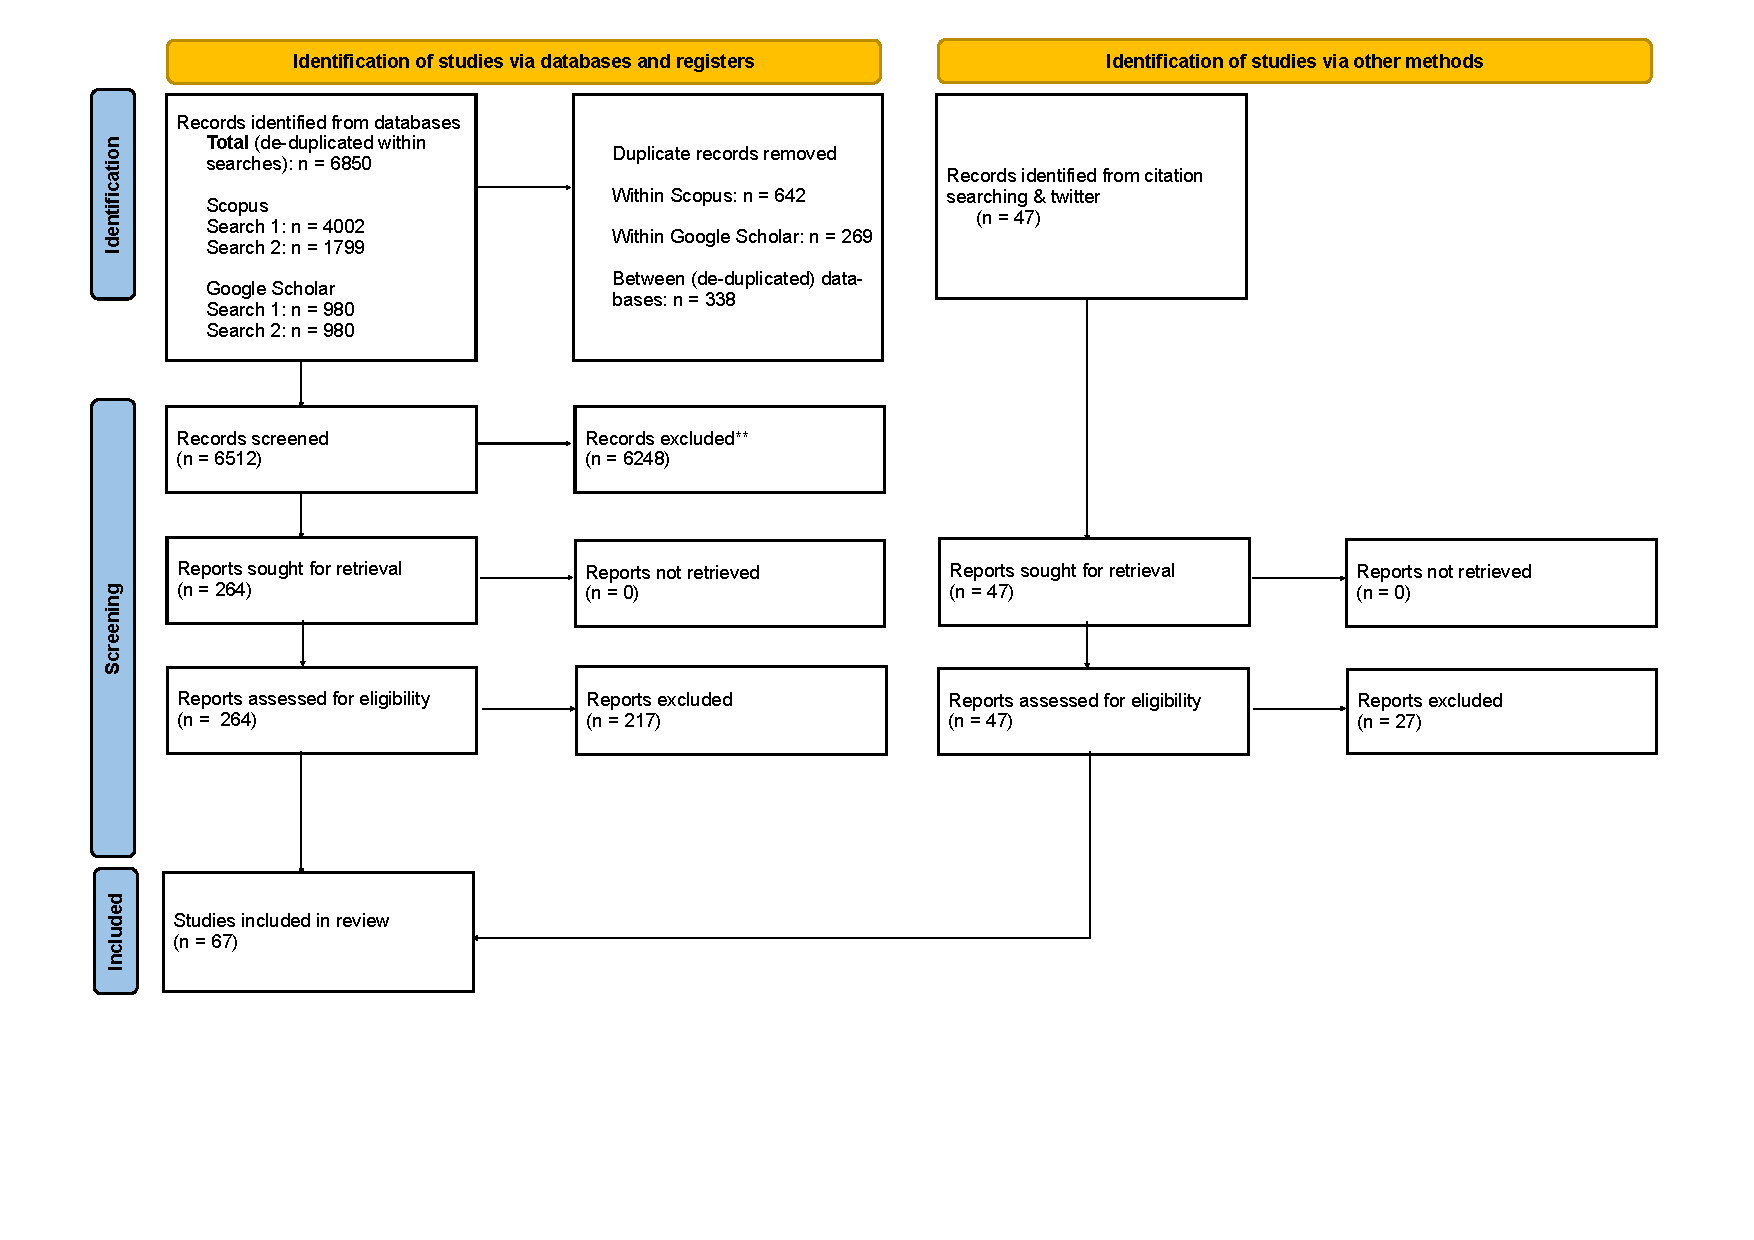
\includegraphics{literature_search/PRISMA_2020_flow_diagram.pdf}
\caption{\label{fig:prisma-flowchart}\emph{PRISMA flow diagram}. A flow diagram for the systematic literature review, based on the 2020 PRISMA template.}
\end{figure}

\subsubsection{Deviations from eligibility criteria}\label{deviations-from-eligibility-criteria}

We followed our eligibility criteria (as outlined above), with 4 exceptions. We rejected one paper based on a criterion that we had not previously set: scale asymmetry.\textsuperscript{65} asked participants: ``According to your knowledge, how do you rate the following headline?'', providing a very asymmetrical set of answer options (``1---not credible; 2---somehow credible; 3---quite credible; 4---credible; 5---very credible''). The paper provides 6 effect sizes, all of which strongly favor our second hypothesis (one effect being as large as d = 2.54). We decided to exclude this paper from our analysis because of its very asymmetric scale (no clear scale midpoint, and labels not symmetrically mapping onto a false/true dichotomy, by contrast to all other response scales included here). Further, we stretched our criterion for real-world news on three instances.\textsuperscript{66} and\textsuperscript{67} used artificial intelligence trained on real-world news to generate false news.\textsuperscript{68} had journalists create the false news items. We reasoned that asking journalists to write news should be similar enough to real-wolrd news, and that LLMs already produce news headlines that are indistinguishable from real news, so it should not make a big difference.

\subsubsection{Literature search}\label{literature-search}

Our literature review is based on two systematic searches. We conducted our first search on March 2, 2023 using Scopus (search string: `\,``false news'' OR ``fake news'' OR ``false stor*'' AND ``accuracy'' OR ``discernment'' OR ``credibilit*'' OR ``belief'' OR ``susceptib*''\,') and google scholar (search string: `\,``Fake news'' \textbar{} ``False news''\textbar{}``False stor*'' ``Accuracy'' \textbar{} ``Discernment''\textbar{}``Credibility''\textbar{}``Belief''\textbar{}``Suceptib*'', no citations, no patents'). On Scopus, given the initially high volume of papers (12425), we excluded papers not written in English, that were not articles or conference papers, and that were from disciplines that are likely irrelevant for the present search (e.g., Dentistry, Veterinary, Chemical Engineering, Chemistry, Nursing, Pharmacology, Microbiology, Materials Science, Medicine) or unlikely to use an experimental design (e.g.~Computer Science, Engineering, Mathematics, see Appendix \ref{lit-review} for detailed search string). After these filters were applied, we ended up with 4002 results. The Google Scholar search was intended to identify important pre-prints or working papers that the Scopus search would have missed. We only considered the first 980 results of that search--a limit imposed by the ``Publish or Perish'' software we used to store Google Scholar search results in a data frame.

After submitting a manuscript version, reviewers remarked that not including the terms ``misinformation'' or ``disinformation'' in our search string might have omitted relevant results. On March 22nd, 2024, we therefor conducted a second, pre-registered (\url{https://osf.io/yn6r2}) search using an extended query string (search string for both Scopus and Google Scholar: `\,``false news'' OR ``fake news'' OR ``false stor*'' OR ``misinformation'' OR ``disinformation'' ) AND ( ``accuracy'' OR ``discernment'' OR ``credibilit*'' OR ``belief'' OR ``suceptib*'' OR ``reliab*'' OR ``vulnerabi*''\,'; see Appendix \ref{lit-review} for detailed search string). After removing duplicates--642 between the first and the second Scopus search and 269 between the first and the second Google Scholar search--the second search yielded an additional 1157 results for Scopus and 711 results for Google Scholar. In total, the Scopus searches yielded 5159, the Google Scholar searches 1691 unique results.

We identified and removed 338 duplicates between the Google Scholar and the Scopus searches and ended up with 6512 documents for screening. We had two screening phases: first titles, second abstracts. Both authors screened the results independently. In case of conflicting decisions, an article passed onto the next stage (i.e.~receive abstract screening or full text assessment). Screening was done based on titles and abstracts only, so that the screeners would not be influenced by information on the authors or the publishing journal. The vast majority of documents (6248) had irrelevant titles and were removed during that phase. Most irrelevant titles were not about false news or misinformation (e.g.~``Formation of a tourist destination image: Co-occurrence analysis of destination promotion videos''), and some were about false news or misinformation but were not about belief or accuracy (e.g.~``Freedom of Expression and Misinformation Laws During the COVID-19 Pandemic and the European Court of Human Rights''). We stored the remaining 264 records in the reference management system Zotero for retrieval. Of those, we rejected a total of 217 papers that did not meet our inclusion criteria. We rejected 87 papers based on their abstract and 130 after assessment of the full text. We documented all rejection decisions, available on the \href{https://osf.io/96zbp/?view_only=d2f3147f652e44e2a0414d7d6d9a6c29}{OSF project page}. We included the remaining 47 papers from the systematic literature search. To complement the systematic search results, we conducted forward and backward citation search through Google Scholar. We also reviewed additional studies that we had on our computers and papers we found scrolling through twitter (mostly unpublished manuscripts). Taken together, we identified an additional 47 papers via those methods. Of these, we excluded 27 papers after full text assessment because they did not meet our inclusion criteria. For these papers, too, we documented our exclusion decisions. They can be found together with the ones of the systematic search on the \href{https://osf.io/96zbp/?view_only=d2f3147f652e44e2a0414d7d6d9a6c29}{OSF project page}. We included the remaining 20 papers. In total, we included 67 papers in our meta analysis, 47 of which were peer-reviewed and 20 grey literature (reports and working papers). We retrieved the relevant summary statistics directly from the paper for 21 papers, calculated them ourselves based on publicly available raw data for 31 papers, and got them from the authors after request for 15 papers.

\subsection{Statistical methods}\label{statistical-methods}

All data and code are publicly available on the \href{https://osf.io/96zbp/?view_only=d2f3147f652e44e2a0414d7d6d9a6c29}{OSF project page}. Unless explicitly stated otherwise, we pre-registered (\url{https://osf.io/svc7u}) all reported analyses. Our choice of statistical models was informed by simulations, which can also be found on the \href{https://osf.io/96zbp/?view_only=d2f3147f652e44e2a0414d7d6d9a6c29}{OSF project page}. We conducted all analyses in R\textsuperscript{69} using Rstudio\textsuperscript{70} and the \texttt{tidyverse} package\textsuperscript{71}. For effect size calculations, we rely on the \texttt{escalc()}, for models on the \texttt{rma.mv()}, for clustered standard errors on the \texttt{robust()} function, all from the \texttt{metafor} package\textsuperscript{72}.

\subsubsection{Deviations from pre-registration}\label{deviations-from-pre-registration}

We pre-registered standardized mean changes using change score standardization (SMCC) as an estimator for our effect sizes\textsuperscript{73}. However, in line with Cochrane guidelines\textsuperscript{33}, we chose to rely on the more common Cohen's d for the main analysis. We report the pre-registered SMCC (along with other alternative estimators) in Appendix \ref{effect-sizes}. All estimators yield similar results. We did not pre-register considering scale symmetry, proportion of true news and false news selection (taken from fact checking sites vs.~verified by researchers) as moderator variables. We report the results regarding these variables in Appendix \ref{moderators}.

\subsubsection{Outcomes}\label{outcomes}

We have two complementary measures of assessing the quality of people's news judgment. The first measure is discernment. It measures the overall quality of news judgment across true and false news. We calculate discernment by subtracting the mean accuracy ratings of false news from the mean accuracy ratings of true news, such that more positive scores indicate better discernment. However, discernment is a limited diagnostic of the quality of people's news judgment. Imagine a study A in which participants rate 50\% of true news and 20\% of false news as accurate, and a study B finding 80\% of true news and 50\% of false news rated as accurate. In both cases, the discernment is the same: Participants rated true news as more accurate by 30 percentage points than false news. However, the performance by news type is very different. In study A, people do well for false news - they only mistakenly classify 20\% as accurate - but are at chance for true news. In study B, it's the opposite. We therefore use a second measure: skepticism bias. For any given level of discernment, it indicates whether people's judgments were better on true news or on false news, and to what extent. First, we calculate an error for false and true news separately, which we define as the distance of participants' actual ratings to the best possible ratings. For example, for study A, the mean error for true news is 50\% (100\%-50\%), because in the best possible scenario, participants would have classified 100\% of true news as true. The error for false news in Study A is 20\% (20\%-0\%), because the best possible performance for participants would have been to classify 0\% of false news as accurate. We calculate skepticism bias by subtracting the mean error for false news from the mean error for true news. For example, for Study A, the skepticism bias is 30\% (50\%-20\%). A positive skepticism bias indicates that people doubt true news more than they believe false news.

\subsubsection{Effect sizes}\label{effect-sizes}

The studies in our meta analysis used a variety of response scales, including both binary (e.g.~``Do you think the above headline is accurate? - Yes, No'') and continuous ones (e.g.~``To the best of your knowledge, how accurate is the claim in the above headline'' 1 = Not at all accurate, 4 = Very accurate). To be able to compare across the different scales, we calculated standardized effects, i.e.~effects expressed in units of standard deviations. Precisely, we calculated Cohen's d as

\[
\text{Cohen's d} = \frac{\bar{x}_{\text{true}} - \bar{x}_{\text{false}}}{SD_{\text{pooled}}}
\] with

\[
SD_{\text{pooled}} = \sqrt{\frac{SD_{\text{true}}^2+SD_{\text{false}}^2}{2}}
\]

The vast majority of experiments (294 out of 303 effects) in our meta analysis manipulated news veracity within participants, i.e.~having participants rate both false and true news. Following the Cochrane manual, we account for the dependency between ratings that this design generates when calculating the standard error for Cohen's d.~Precisely, we calculate the standard error for within participant designs as

\[
SE_{\text{Cohen's d (within)}} = \sqrt{\frac{2(1-r_{\text{true},\text{false}})}{n}+\frac{\text{Cohen's d}^2}{2n}}
\]

where \(r\) is the correlation between true and false news. Ideally, for each effect size (i.e.~the meta-analytic units of observation) in our data, we need the estimate of \(r\). However, this correlation is generally not reported in the original papers. We could only obtain it for a subset of samples for which we collected the summary statistics ourselves, based on the raw data. Based on this subset of correlations, we calculated an average correlation, which we then imputed for all effect size calculations. This approach is in line with the \href{https://training.cochrane.org/handbook/current/chapter-23\#section-23-2-7-3}{Cochrane recommendations for crossover trials}\textsuperscript{33}. In our case, this average correlation is 0.26.

For the 9 (out of 303) effects from studies that used a between participant design, we calculated the standard error as

\[
SE_{\text{Cohen's d (between)}} = \sqrt{\frac{n_{\text{true}}+n_{\text{false}}}{n_{\text{true}}n_{\text{false}}}+\frac{\text{Cohen's d}^2}{2(n_{\text{true}}+n_{\text{false}})}}
\]

For all effect size calculations, we defined the sample size \(n\) as the number of instances of news ratings. That is, we multiplied the number of participants with the number of news items rated per participant.

\subsubsection{Models}\label{models}

In our models for the meta analysis, each effect size was weighted by the inverse of its standard error, thereby giving more weight to studies with larger sample sizes. We used random effects models, which assume that there is not only one true effect size but a distribution of true effect sizes\textsuperscript{74}. These models assume that variation in effect sizes is not only due to sampling error alone, and thereby allow to model other sources of variance. We estimated the overall effect of our outcome variables using a three-level meta-analytic model with random effects on the sample and the publication level. This approach allowed us to account for the hierarchical structure of our data, in which samples (level three) contribute multiple effects (level two),\textsuperscript{level one being the participant level of the original studies, see 74}. Multiple effects per sample occur, for example, when separate accuracy ratings are available by news topic, or when follow-up studies were conducted on the same participants. However, the multi-level models do not account for dependencies in sampling error. When one same sample contributes several effect sizes, one should expect their respective sampling errors to be correlated\textsuperscript{74}. To account for dependency in sampling errors, we computed cluster-robust standard errors, confidence intervals, and statistical tests for all estimated effect sizes.

To assess the effect of moderator variables, we calculated meta regressions. We calculated a separate regression for each moderator, by adding the moderator variable as a fixed effect to the multilevel meta models presented above. We pre-registered a list of six moderator variables to test. Those included the \emph{country} of studies (levels: United States vs.~all other countries), \emph{political concordance} (levels: politically concordant vs.~politically discordant), \emph{news family} (levels: political, including both concordant and discordant vs.~covid related vs.~other, including categories as diverse as history, environment, health, science and military related news items), the \emph{format} in which the news were presented (levels: headline only vs.~headline and picture vs.~headline, picture and lede), whether news items were accompanied by a \emph{source} or not, and the \emph{response scale} used (levels: 4-point vs.~binary vs.~6-point vs.~7-point vs.~other, for all other numeric scales that were not frequent). We ran an additional regressiosn for two non-preregistered variables, namely the \emph{symmetry of scales} (levels: perfectly symmetrical vs.~imperfectly symmetrical) and \emph{false news selection} (levels: taken from fact check sites vs.~verified by researchers). We further descriptively checked whether the \emph{proportion of true news} among all news would yield differences.

\subsubsection{Publication bias}\label{publication-bias}

We ran some standard procedures for detecting publication bias. However, a priori we did not expect publication bias to be present because our variables of interest were not those of interest to the researchers of the original studies: Researchers generally set out to test factors that alter discernment, and not the state of discernment in the control group. No study measured skepticism bias in the way we define it here.



\begin{figure}
\centering
\includegraphics{output/figures/funnel.pdf}
\caption{\label{fig:funnel}\emph{Funnel plots for discernment and skepticism bias}. Dots represent effect sizes. In the absence of publication bias and heterogeneity, one would then expect to see the points forming a funnel shape, with the majority of the points falling inside of the pseudo-confidence region centered around the average effect estimate, with bounds of ±1.96 SE (the standard error value from the y-axis). The dashed red regression line illustrates the estimate of the Egger's regression test. For both outcomes, the slope differs significantly from zero, see Appendix \ref{publication-bias}.}
\end{figure}

Regarding discernment, we find evidence that smaller studies tend to report larger effect sizes, according to Egger's regression test (see Fig. \ref{fig:funnel}; see also Appendix \ref{publication-bias}). Regarding skepticism bias, we find the opposite. However, it is unclear how meaningful these patterns are. As illustrated by the funnel plot, there is generally high between-effect size heterogeneity: Even when focusing only on the most precise effect sizes (top of the funnel), the estimates vary substantially. It thus seems reasonable to assume that most of the dispersion of effect sizes does not arise from studies' sampling error, but from studies estimating different true effects. Further, even the small studies are relatively high powered, suggesting that they would have yielded significant, publishable results even with smaller effect sizes. Lastly, Egger's regression test can lead to an inflation of false positive results when applied to standardized mean differences\textsuperscript{74,75}. We do not find evidence for asymmetry regarding skepticism bias.



\begin{figure}
\centering
\includegraphics{output/figures/p-curve.pdf}
\caption{\label{fig:p-curve}\emph{P-curves for discernment and skepticism bias}. The p-curve shows the percentage of effect sizes for a given p value within the range of 0.1 and 0.5. All values smaller than 0.01 are rounded to that value. The reference lines indicate the expected percentage of studies for a given p value, assuming that there is a true effect and certain statistical power to detect it (either 0\% or 30\% power). The observed p-curve is negatively sloped and heavily right skewed (the tail points to the right) for both outcomes, which suggests no widespread p-hacking.}
\end{figure}

We do not find any evidence to suspect p-hacking for either discernment or skepticism bias from visually inspecting p-curves for both outcomes (see Fig. \ref{fig:p-curve}).

\section{Data availability}\label{data-availability}

The extracted data used to produce our results are available on the OSF project page (\url{https://osf.io/96zbp/?view_only=d2f3147f652e44e2a0414d7d6d9a6c29}).

\section{Code availability}\label{code-availability}

The code used to create all results (including tables and figures) of this manuscript is also available on the OSF project page (\url{https://osf.io/96zbp/?view_only=d2f3147f652e44e2a0414d7d6d9a6c29}).

\section{Acknowledgements}\label{acknowledgements}

We thank Aurélien Allard, Hugo Mercier, Gordon Pennycook, Ariana Modirrousta-Galian and Ben Tappin for their valuable feedback on earlier versions of the manuscript.

\section{Author Contributions Statement}\label{author-contributions-statement}

\emph{Jan Pfänder}: Conceptualization, Systematic literature search, Methodology, Software, Formal Analysis, Data curation, Visualization, Writing - Original draft, Writing - Review \& Editing. \emph{Sacha Altay}: Conceptualization, Methodology, Writing - Original draft, Writing - Review \& Editing.

\section{Competing interest}\label{competing-interest}

The authors declare having no competing interests.

\FloatBarrier

\newpage

\section{References}\label{references}

\begingroup
\setlength{\parindent}{-0.5in}
\setlength{\leftskip}{0.5in}

References marked with an asterisk indicate studies included in the meta-analysis.

\phantomsection\label{refs}
\begin{CSLReferences}{0}{0}
\bibitem[\citeproctext]{ref-egelhoferPopulistAttitudesPoliticians2022}
\CSLLeftMargin{1. }%
\CSLRightInline{Egelhofer, J. L., Boyer, M., Lecheler, S. \& Aaldering, L. \href{https://doi.org/10.1093/joc/jqac031}{Populist attitudes and politicians{'} disinformation accusations: effects on perceptions of media and politicians}. \emph{Journal of Communication} \textbf{72}, 619--632 (2022).}

\bibitem[\citeproctext]{ref-brennenLieDetectionWhat2023}
\CSLLeftMargin{2. }%
\CSLRightInline{Brennen, T. \& Magnussen, S. Lie Detection: What Works? \emph{Current Directions in Psychological Science} 096372142311730 (2023) doi:\href{https://doi.org/10.1177/09637214231173095}{10.1177/09637214231173095}.}

\bibitem[\citeproctext]{ref-montalverneTrustGapHow2022}
\CSLLeftMargin{3. }%
\CSLRightInline{Mont'Alverne, C. \emph{et al.} The trust gap: How and why news on digital platforms is viewed more sceptically versus news in general. (2022).}

\bibitem[\citeproctext]{ref-metzgerMakingSenseCredibility2007}
\CSLLeftMargin{4. }%
\CSLRightInline{Metzger, M. J. \href{https://doi.org/10.1002/asi.20672}{Making sense of credibility on the Web: Models for evaluating online information and recommendations for future research}. \emph{Journal of the American Society for Information Science and Technology} \textbf{58}, 2078--2091 (2007).}

\bibitem[\citeproctext]{ref-rossarguedasSnapJudgementsHow2022}
\CSLLeftMargin{5. }%
\CSLRightInline{Ross Arguedas, A. \emph{et al.} Snap judgements: How audiences who lack trust in news navigate information on digital platforms. (2022).}

\bibitem[\citeproctext]{ref-altayExposureHigherRates2023}
\CSLLeftMargin{6. }%
\CSLRightInline{Altay, S., Lyons, B. \& Modirrousta-Galian, A. Exposure to higher rates of false news erodes media trust and fuels skepticism in news judgment. doi:\href{https://doi.org/10.31234/osf.io/t9r43}{10.31234/osf.io/t9r43}.}

\bibitem[\citeproctext]{ref-bryanovDeterminantsIndividualsBelief2021}
\CSLLeftMargin{7. }%
\CSLRightInline{Bryanov, K. \& Vziatysheva, V. \href{https://doi.org/10.1371/journal.pone.0253717}{Determinants of individuals{'} belief in fake news: A scoping review determinants of belief in fake news}. \emph{PLOS ONE} \textbf{16}, e0253717 (2021).}

\bibitem[\citeproctext]{ref-pennycookLazyNotBiased2019}
\CSLLeftMargin{8. }%
\CSLRightInline{*Pennycook, G. \& Rand, D. G. \href{https://doi.org/10.1016/j.cognition.2018.06.011}{Lazy, not biased: Susceptibility to partisan fake news is better explained by lack of reasoning than by motivated reasoning}. \emph{Cognition} \textbf{188}, 39--50 (2019).}

\bibitem[\citeproctext]{ref-schulzAreNewsOutlets2020}
\CSLLeftMargin{9. }%
\CSLRightInline{Schulz, A., Fletcher, R. \& Popescu, M. Are news outlets viewed in the same way by experts and the public? A comparison across 23 european countries. \emph{Reuters Institute for the Study of Journalism} (2020).}

\bibitem[\citeproctext]{ref-mouraoFakeNewsDiscursive2019}
\CSLLeftMargin{10. }%
\CSLRightInline{Mourão, R. R. \& Robertson, C. T. \href{https://doi.org/10.1080/1461670X.2019.1566871}{Fake News as Discursive Integration: An Analysis of Sites That Publish False, Misleading, Hyperpartisan and Sensational Information}. \emph{Journalism Studies} \textbf{20}, 2077--2095 (2019).}

\bibitem[\citeproctext]{ref-vosoughiSpreadTrueFalse2018a}
\CSLLeftMargin{11. }%
\CSLRightInline{Vosoughi, S., Roy, D. \& Aral, S. \href{https://doi.org/10.1126/science.aap9559}{The spread of true and false news online}. \emph{Science} \textbf{359}, 1146--1151 (2018).}

\bibitem[\citeproctext]{ref-chenWhatMakesNews2023}
\CSLLeftMargin{12. }%
\CSLRightInline{*Chen, X., Pennycook, G. \& Rand, D. What makes news sharable on social media? \emph{Journal of Quantitative Description: Digital Media} \textbf{3}, (2023).}

\bibitem[\citeproctext]{ref-altayIfThisAccount2022}
\CSLLeftMargin{13. }%
\CSLRightInline{*Altay, S., Araujo, E. de \& Mercier, H. \href{https://doi.org/10.1080/21670811.2021.1941163}{{``}If This account is True, It is Most Enormously Wonderful{''}: Interestingness-If-True and the Sharing of True and False News}. \emph{Digital Journalism} \textbf{10}, 373--394 (2022).}

\bibitem[\citeproctext]{ref-acerbiResearchNoteFighting2022}
\CSLLeftMargin{14. }%
\CSLRightInline{Acerbi, A., Altay, S. \& Mercier, H. Research note: Fighting misinformation or fighting for information? \emph{Harvard Kennedy School Misinformation Review} (2022) doi:\href{https://doi.org/10.37016/mr-2020-87}{10.37016/mr-2020-87}.}

\bibitem[\citeproctext]{ref-mercierNotBornYesterday2020}
\CSLLeftMargin{15. }%
\CSLRightInline{Mercier, H. \emph{\href{https://doi.org/10.1515/9780691198842}{Not born yesterday: the science of who we trust and what we believe}}. (2020).}

\bibitem[\citeproctext]{ref-brashierJudgingTruth2020}
\CSLLeftMargin{16. }%
\CSLRightInline{Brashier, N. M. \& Marsh, E. J. \href{https://doi.org/10.1146/annurev-psych-010419-050807}{Judging Truth}. \emph{Annual Review of Psychology} \textbf{71}, 499--515 (2020).}

\bibitem[\citeproctext]{ref-streetSourceTruthBias2015}
\CSLLeftMargin{17. }%
\CSLRightInline{Street, C. N. H. \& Masip, J. \href{https://doi.org/10.1111/sjop.12204}{The source of the truth bias: Heuristic processing?} \emph{Scandinavian Journal of Psychology} \textbf{56}, 254--263 (2015).}

\bibitem[\citeproctext]{ref-levineTruthDefaultTheoryTDT2014}
\CSLLeftMargin{18. }%
\CSLRightInline{Levine, T. R. \href{https://doi.org/10.1177/0261927X14535916}{Truth-Default Theory (TDT): A Theory of Human Deception and Deception Detection}. \emph{Journal of Language and Social Psychology} \textbf{33}, 378--392 (2014).}

\bibitem[\citeproctext]{ref-newmanReutersInstituteDigital2022}
\CSLLeftMargin{19. }%
\CSLRightInline{Newman, N., Fletcher, R., Robertson, C. T., Eddy, K. \& Nielsen, R. K. Reuters Institute Digital News Report 2022. (2022).}

\bibitem[\citeproctext]{ref-mihailidisCostDisbeliefFracturing2021}
\CSLLeftMargin{20. }%
\CSLRightInline{Mihailidis, P. \& Foster, B. \href{https://doi.org/10.1177/0002764220978470}{The Cost of Disbelief: Fracturing News Ecosystems in an Age of Rampant Media Cynicism}. \emph{American Behavioral Scientist} \textbf{65}, 616--631 (2021).}

\bibitem[\citeproctext]{ref-egelhoferFakeNewsTwodimensional2019}
\CSLLeftMargin{21. }%
\CSLRightInline{Egelhofer, J. L. \& Lecheler, S. \href{https://doi.org/10.1080/23808985.2019.1602782}{Fake news as a two-dimensional phenomenon: a framework and research agenda}. \emph{Annals of the International Communication Association} \textbf{43}, 97--116 (2019).}

\bibitem[\citeproctext]{ref-vanduynPrimingFakeNews2019}
\CSLLeftMargin{22. }%
\CSLRightInline{Van Duyn, E. \& Collier, J. \href{https://doi.org/10.1080/15205436.2018.1511807}{Priming and Fake News: The Effects of Elite Discourse on Evaluations of News Media}. \emph{Mass Communication and Society} \textbf{22}, 29--48 (2019).}

\bibitem[\citeproctext]{ref-paulRussianFirehoseFalsehood2016}
\CSLLeftMargin{23. }%
\CSLRightInline{Paul, C. \& Matthews, M. The russian {``}firehose of falsehood{''} propaganda model. \emph{Rand Corporation} \textbf{2}, 1--10 (2016).}

\bibitem[\citeproctext]{ref-ulusoyFloodingZoneHow2021}
\CSLLeftMargin{24. }%
\CSLRightInline{Ulusoy, E. \emph{et al.} Flooding the zone: How exposure to implausible statements shapes subsequent belief judgments. \emph{International Journal of Public Opinion Research} \textbf{33}, 856--872 (2021).}

\bibitem[\citeproctext]{ref-fletcherPeopleDontTrust2017}
\CSLLeftMargin{25. }%
\CSLRightInline{Fletcher, R. \& Nielsen, R.-K. People dont trust news media{\textendash}and this is key to the global misinformation debate. \emph{AA. VV., Understanding and Addressing the Disinformation Ecosystem} 13--17 (2017).}

\bibitem[\citeproctext]{ref-luoCredibilityPerceptionsDetection2022}
\CSLLeftMargin{26. }%
\CSLRightInline{*Luo, M., Hancock, J. T. \& Markowitz, D. M. \href{https://doi.org/10.1177/0093650220921321}{Credibility Perceptions and Detection Accuracy of Fake News Headlines on Social Media: Effects of Truth-Bias and Endorsement Cues}. \emph{Communication Research} \textbf{49}, 171--195 (2022).}

\bibitem[\citeproctext]{ref-bataillerSignalDetectionApproach2022}
\CSLLeftMargin{27. }%
\CSLRightInline{Batailler, C., Brannon, S. M., Teas, P. E. \& Gawronski, B. \href{https://doi.org/10.1177/1745691620986135}{A Signal Detection Approach to Understanding the Identification of Fake News}. \emph{Perspectives on Psychological Science} \textbf{17}, 78--98 (2022).}

\bibitem[\citeproctext]{ref-modirrousta-galianGamifiedInoculationInterventions2023}
\CSLLeftMargin{28. }%
\CSLRightInline{Modirrousta-Galian, A. \& Higham, P. A. Gamified inoculation interventions do not improve discrimination between true and fake news: Reanalyzing existing research with receiver operating characteristic analysis. \emph{Journal of Experimental Psychology: General} (2023).}

\bibitem[\citeproctext]{ref-diasEmphasizingPublishersDoes2020}
\CSLLeftMargin{29. }%
\CSLRightInline{*Dias, N., Pennycook, G. \& Rand, D. G. Emphasizing publishers does not effectively reduce susceptibility to misinformation on social media. \emph{Harvard Kennedy School Misinformation Review} (2020) doi:\href{https://doi.org/10.37016/mr-2020-001}{10.37016/mr-2020-001}.}

\bibitem[\citeproctext]{ref-tappinBayesianBiasedAnalytic2020}
\CSLLeftMargin{30. }%
\CSLRightInline{Tappin, B. M., Pennycook, G. \& Rand, D. G. \href{https://doi.org/10.1016/j.cognition.2020.104375}{Bayesian or biased? Analytic thinking and political belief updating}. \emph{Cognition} \textbf{204}, 104375 (2020).}

\bibitem[\citeproctext]{ref-calvilloInitialAccuracyFocus2020}
\CSLLeftMargin{31. }%
\CSLRightInline{Calvillo, D. P. \& Smelter, T. J. \href{https://doi.org/10.1186/s41235-020-00257-y}{An initial accuracy focus reduces the effect of prior exposure on perceived accuracy of news headlines}. \emph{Cognitive Research: Principles and Implications} \textbf{5}, 55 (2020).}

\bibitem[\citeproctext]{ref-guayHowThinkWhether2023}
\CSLLeftMargin{32. }%
\CSLRightInline{Guay, B., Berinsky, A. J., Pennycook, G. \& Rand, D. \href{https://doi.org/10.1038/s41562-023-01667-w}{How to think about whether misinformation interventions work}. \emph{Nature Human Behaviour} \textbf{7}, 1231--1233 (2023).}

\bibitem[\citeproctext]{ref-higgins_cochrane_2019}
\CSLLeftMargin{33. }%
\CSLRightInline{Higgins, J. P. \emph{et al.} \emph{Cochrane handbook for systematic reviews of interventions}. (John Wiley \& Sons, 2019).}

\bibitem[\citeproctext]{ref-pennycook2021}
\CSLLeftMargin{34. }%
\CSLRightInline{Pennycook, G. \emph{et al.} \href{https://doi.org/10.1038/s41586-021-03344-2}{Shifting attention to accuracy can reduce misinformation online}. \emph{Nature} \textbf{592}, 590--595 (2021).}

\bibitem[\citeproctext]{ref-rathje2023}
\CSLLeftMargin{35. }%
\CSLRightInline{Rathje, S., Roozenbeek, J., Van Bavel, J. J. \& Van Der Linden, S. Accuracy and social motivations shape judgements of (mis)information. \emph{Nature Human Behaviour} (2023) doi:\href{https://doi.org/10.1038/s41562-023-01540-w}{10.1038/s41562-023-01540-w}.}

\bibitem[\citeproctext]{ref-capraroThinkThisNews}
\CSLLeftMargin{36. }%
\CSLRightInline{Capraro, V. \& Celadin, T. {``}I Think This News Is Accurate{''}: Endorsing Accuracy Decreases the Sharing of Fake News and Increases the Sharing of Real News. \emph{Personality and Social Psychology Bulletin}.}

\bibitem[\citeproctext]{ref-globigChangingIncentiveStructure2023}
\CSLLeftMargin{37. }%
\CSLRightInline{Globig, L. K., Holtz, N. \& Sharot, T. \href{https://doi.org/10.7554/eLife.85767}{Changing the incentive structure of social media platforms to halt the spread of misinformation}. \emph{eLife} \textbf{12}, e85767 (2023).}

\bibitem[\citeproctext]{ref-epsteinSocialMediaContext2023}
\CSLLeftMargin{38. }%
\CSLRightInline{*Epstein, Z., Sirlin, N., Arechar, A., Pennycook, G. \& Rand, D. The social media context interferes with truth discernment. \emph{Science Advances} \textbf{9}, eabo6169 (2023).}

\bibitem[\citeproctext]{ref-modirrousta-galianWordlessWisdomDominant2023}
\CSLLeftMargin{39. }%
\CSLRightInline{Modirrousta-Galian, A., Higham, P. A. \& Seabrooke, T. \emph{Wordless Wisdom: The Dominant Role of Tacit Knowledge in True and Fake News Discrimination}. \url{https://osf.io/2gubk} (2023) doi:\href{https://doi.org/10.31234/osf.io/2gubk}{10.31234/osf.io/2gubk}.}

\bibitem[\citeproctext]{ref-allenScalingFactcheckingUsing2021}
\CSLLeftMargin{40. }%
\CSLRightInline{*Allen, J., Arechar, A. A., Pennycook, G. \& Rand, D. G. Scaling up fact-checking using the wisdom of crowds. \emph{Science advances} \textbf{7}, eabf4393 (2021).}

\bibitem[\citeproctext]{ref-martelCrowdsCanEffectively2022}
\CSLLeftMargin{41. }%
\CSLRightInline{Martel, C., Allen, J. N. L., Pennycook, G. \& Rand, D. G. \emph{Crowds Can Effectively Identify Misinformation at Scale}. \url{https://osf.io/2tjk7} (2022) doi:\href{https://doi.org/10.31234/osf.io/2tjk7}{10.31234/osf.io/2tjk7}.}

\bibitem[\citeproctext]{ref-hoesLeveragingChatGPTEfficient2023}
\CSLLeftMargin{42. }%
\CSLRightInline{Hoes, E., Altay, S. \& Bermeo, J. Leveraging ChatGPT for Efficient Fact-Checking. doi:\href{https://doi.org/10.31234/osf.io/qnjkf}{10.31234/osf.io/qnjkf}.}

\bibitem[\citeproctext]{ref-altayMisinformationMisinformationConceptual}
\CSLLeftMargin{43. }%
\CSLRightInline{Altay, S., Berriche, M. \& Acerbi, A. Misinformation on Misinformation: Conceptual and Methodological Challenges. \emph{Social Media}.}

\bibitem[\citeproctext]{ref-allenEvaluatingFakeNews2020}
\CSLLeftMargin{44. }%
\CSLRightInline{Allen, J., Howland, B., Mobius, M., Rothschild, D. \& Watts, D. J. Evaluating the fake news problem at the scale of the information ecosystem. \emph{Science Advances} \textbf{6}, eaay3539 (2020).}

\bibitem[\citeproctext]{ref-altayNewsParticipationDeclining2024}
\CSLLeftMargin{45. }%
\CSLRightInline{Altay, S., Fletcher, R. \& Nielsen, R. K. News participation is declining: Evidence from 46 countries between 2015 and 2022. \emph{New Media \& Society} 14614448241247822 (2024) doi:\href{https://doi.org/10.1177/14614448241247822}{10.1177/14614448241247822}.}

\bibitem[\citeproctext]{ref-newmanDigitalNewsReport2023}
\CSLLeftMargin{46. }%
\CSLRightInline{Newman, N., Fletcher, R., Eddy, K., Robertson, C. T. \& Nielsen, R. K. Digital news report 2023. (2023).}

\bibitem[\citeproctext]{ref-altaySkepticismFramingMedia2023}
\CSLLeftMargin{47. }%
\CSLRightInline{Altay, S., De Angelis, A. \& Hoes, E. Beyond skepticism: Framing media literacy tips to promote reliable informatio. doi:\href{https://doi.org/10.31234/osf.io/5gckb}{10.31234/osf.io/5gckb}.}

\bibitem[\citeproctext]{ref-guayHowThinkWhether2022}
\CSLLeftMargin{48. }%
\CSLRightInline{Guay, B., Berinsky, A., Pennycook, G. \& Rand, D. How to think about whether misinformation interventions work. doi:\href{https://doi.org/10.31234/osf.io/gv8qx}{10.31234/osf.io/gv8qx}.}

\bibitem[\citeproctext]{ref-highamMeanRatingDifference2024a}
\CSLLeftMargin{49. }%
\CSLRightInline{Higham, P. A., Modirrousta-Galian, A. \& Seabrooke, T. \href{https://doi.org/10.1016/j.copsyc.2023.101785}{Mean rating difference scores are poor measures of discernment: The role of response criteria}. \emph{Current Opinion in Psychology} \textbf{56}, 101785 (2024).}

\bibitem[\citeproctext]{ref-hoesProminentMisinformationInterventions2023}
\CSLLeftMargin{50. }%
\CSLRightInline{Hoes, E., Aitken, B., Zhang, J., Gackowski, T. \& Wojcieszak, M. \emph{Prominent misinformation interventions reduce misperceptions but increase skepticism}. \url{https://osf.io/zmpdu} (2023) doi:\href{https://doi.org/10.31234/osf.io/zmpdu}{10.31234/osf.io/zmpdu}.}

\bibitem[\citeproctext]{ref-bachmannStudyingDownstreamEffects2023}
\CSLLeftMargin{51. }%
\CSLRightInline{Bachmann, I. \& Valenzuela, S. \href{https://doi.org/10.1177/20563051231179694}{Studying the Downstream Effects of Fact-Checking on Social Media: Experiments on Correction Formats, Belief Accuracy, and Media Trust}. \emph{Social Media + Society} \textbf{9}, 20563051231179694 (2023).}

\bibitem[\citeproctext]{ref-hillAcquiescenceBiasInflates2023}
\CSLLeftMargin{52. }%
\CSLRightInline{Hill, S. J. \& Roberts, M. E. \href{https://doi.org/10.1017/pan.2022.28}{Acquiescence Bias Inflates Estimates of Conspiratorial Beliefs and Political Misperceptions}. \emph{Political Analysis} \textbf{31}, 575--590 (2023).}

\bibitem[\citeproctext]{ref-alperWhenConspiracyTheories2021}
\CSLLeftMargin{53. }%
\CSLRightInline{Alper, S. When conspiracy theories make sense: The role of social inclusiveness.}

\bibitem[\citeproctext]{ref-besaluCredibilityDigitalPolitical2021}
\CSLLeftMargin{54. }%
\CSLRightInline{Besalú, R. \& Pont-Sorribes, C. \href{https://doi.org/10.3390/socsci10050170}{Credibility of Digital Political News in Spain: Comparison between Traditional Media and Social Media}. \emph{Social Sciences} \textbf{10}, 170 (2021).}

\bibitem[\citeproctext]{ref-karlsenSocialMediaTrust2023}
\CSLLeftMargin{55. }%
\CSLRightInline{Karlsen, R. \& Aalberg, T. \href{https://doi.org/10.1080/21670811.2021.1945938}{Social Media and Trust in News: An Experimental Study of the Effect of Facebook on News Story Credibility}. \emph{Digital Journalism} \textbf{11}, 144--160 (2023).}

\bibitem[\citeproctext]{ref-agadjanianPlatformPenaltyNews2023}
\CSLLeftMargin{56. }%
\CSLRightInline{Agadjanian, A. \emph{et al.} A platform penalty for news? How social media context can alter information credibility online. \emph{Journal of Information Technology \& Politics} \textbf{20}, 338--348 (2023).}

\bibitem[\citeproctext]{ref-gawronskiTruthSensitivityPartisan2023}
\CSLLeftMargin{57. }%
\CSLRightInline{*Gawronski, B., Ng, N. L. \& Luke, D. M. \href{https://doi.org/10.1037/xge0001381}{Truth sensitivity and partisan bias in responses to misinformation.} \emph{Journal of Experimental Psychology: General} \textbf{152}, 2205--2236 (2023).}

\bibitem[\citeproctext]{ref-troucheVigilantConservatismEvaluating2018}
\CSLLeftMargin{58. }%
\CSLRightInline{Trouche, E., Johansson, P., Hall, L. \& Mercier, H. \href{https://doi.org/10.1371/journal.pone.0188825}{Vigilant conservatism in evaluating communicated information}. \emph{PLOS ONE} \textbf{13}, e0188825 (2018).}

\bibitem[\citeproctext]{ref-altayQuantifyingInfodemicPeople2022}
\CSLLeftMargin{59. }%
\CSLRightInline{Altay, S., Kleis Nielsen, R. \& Fletcher, R. \href{https://doi.org/10.51685/jqd.2022.020}{Quantifying the {``}infodemic{''}: People turned to trustworthy news outlets during the 2020 coronavirus pandemic}. \emph{Journal of Quantitative Description: Digital Media} \textbf{2}, (2022).}

\bibitem[\citeproctext]{ref-altayWhyFewPeople2022}
\CSLLeftMargin{60. }%
\CSLRightInline{Altay, S., Hacquin, A.-S. \& Mercier, H. \href{https://doi.org/10.1177/1461444820969893}{Why do so few people share fake news? It hurts their reputation}. \emph{New Media \& Society} \textbf{24}, 1303--1324 (2022).}

\bibitem[\citeproctext]{ref-garrettConservativesSusceptibilityPolitical2021}
\CSLLeftMargin{61. }%
\CSLRightInline{*Garrett, R. K. \& Bond, R. M. \href{https://doi.org/10.1126/sciadv.abf1234}{Conservatives{'} susceptibility to political misperceptions}. \emph{Science Advances} \textbf{7}, eabf1234 (2021).}

\bibitem[\citeproctext]{ref-aslettOnlineSearchesEvaluate2024}
\CSLLeftMargin{62. }%
\CSLRightInline{*Aslett, K. \emph{et al.} \href{https://doi.org/10.1038/s41586-023-06883-y}{Online searches to evaluate misinformation can increase its perceived veracity}. \emph{Nature} \textbf{625}, 548--556 (2024).}

\bibitem[\citeproctext]{ref-pennycookPracticalGuideDoing2021}
\CSLLeftMargin{63. }%
\CSLRightInline{*Pennycook, G., Binnendyk, J., Newton, C. \& Rand, D. G. \href{https://doi.org/10.1525/collabra.25293}{A Practical Guide to Doing Behavioral Research on Fake News and Misinformation}. \emph{Collabra: Psychology} \textbf{7}, 25293 (2021).}

\bibitem[\citeproctext]{ref-page2021}
\CSLLeftMargin{64. }%
\CSLRightInline{Page, M. J. \emph{et al.} \href{https://doi.org/10.1136/bmj.n71}{The PRISMA 2020 statement: an updated guideline for reporting systematic reviews}. \emph{BMJ} \textbf{372}, n71 (2021).}

\bibitem[\citeproctext]{ref-baptistaInfluencePoliticalIdeology2021}
\CSLLeftMargin{65. }%
\CSLRightInline{Baptista, J. P., Correia, E., Gradim, A. \& Piñeiro-Naval, V. \href{https://doi.org/10.3390/publications9020023}{The Influence of Political Ideology on Fake News Belief: The Portuguese Case}. \emph{Publications} \textbf{9}, 23 (2021).}

\bibitem[\citeproctext]{ref-maertensMisinformationSusceptibilityTest2021}
\CSLLeftMargin{66. }%
\CSLRightInline{*Maertens, R. \emph{et al.} \emph{The Misinformation Susceptibility Test (MIST): A psychometrically validated measure of news veracity discernment}. \url{https://osf.io/gk68h} (2021) doi:\href{https://doi.org/10.31234/osf.io/gk68h}{10.31234/osf.io/gk68h}.}

\bibitem[\citeproctext]{ref-roozenbeekSusceptibilityMisinformationCOVID192020}
\CSLLeftMargin{67. }%
\CSLRightInline{*Roozenbeek, J. \emph{et al.} \href{https://doi.org/10.1098/rsos.201199}{Susceptibility to misinformation about COVID-19 around the world}. \emph{Royal Society Open Science} \textbf{7}, 201199 (2020).}

\bibitem[\citeproctext]{ref-bryanovWhatDrivesPerceptions2023}
\CSLLeftMargin{68. }%
\CSLRightInline{*Bryanov, K. \emph{et al.} \href{https://doi.org/10.1080/10584609.2023.2172492}{What Drives Perceptions of Foreign News Coverage Credibility? A Cross-National Experiment Including Kazakhstan, Russia, and Ukraine}. \emph{Political Communication} \textbf{40}, 115--146 (2023).}

\bibitem[\citeproctext]{ref-rcoreteam2022}
\CSLLeftMargin{69. }%
\CSLRightInline{R Core Team. \emph{\href{https://www.R-project.org/}{R: A language and environment for statistical computing}}. (R Foundation for Statistical Computing, 2022).}

\bibitem[\citeproctext]{ref-positteam2023}
\CSLLeftMargin{70. }%
\CSLRightInline{Posit team. \emph{\href{http://www.posit.co/}{RStudio: Integrated development environment for r}}. (Posit Software, PBC, 2023).}

\bibitem[\citeproctext]{ref-wickham2019}
\CSLLeftMargin{71. }%
\CSLRightInline{Wickham, H. \emph{et al.} \href{https://doi.org/10.21105/joss.01686}{Welcome to the tidyverse}. \emph{Journal of Open Source Software} \textbf{4}, 1686 (2019).}

\bibitem[\citeproctext]{ref-viechtbauer_conducting_2010}
\CSLLeftMargin{72. }%
\CSLRightInline{Viechtbauer, W. \href{https://doi.org/10.18637/jss.v036.i03}{Conducting meta-analyses in \emph{r} with the \textbf{metafor} package}. \emph{J. Stat. Soft.} \textbf{36}, (2010).}

\bibitem[\citeproctext]{ref-gibbons_estimation_1993}
\CSLLeftMargin{73. }%
\CSLRightInline{Gibbons, R. D., Hedeker, D. R. \& Davis, J. M. \href{https://doi.org/10.3102/10769986018003271}{Estimation of effect size from a series of experiments involving paired comparisons}. \emph{Journal of Educational Statistics} \textbf{18}, 271--279 (1993).}

\bibitem[\citeproctext]{ref-harrer2021}
\CSLLeftMargin{74. }%
\CSLRightInline{Harrer, M., Cuijpers, P., A, F. T. \& Ebert, D. D. \emph{Doing meta-analysis with r: A hands-on guide}. (Chapman \& Hall/CRC Press, 2021).}

\bibitem[\citeproctext]{ref-pustejovsky2019}
\CSLLeftMargin{75. }%
\CSLRightInline{Pustejovsky, J. E. \href{https://www.jepusto.com/simulating-correlated-smds/}{Simulating correlated standardized mean differences for meta-analysis}. (2019).}

\bibitem[\citeproctext]{ref-hedges_distribution_1981}
\CSLLeftMargin{76. }%
\CSLRightInline{Hedges, L. V. \href{https://doi.org/10.3102/10769986006002107}{Distribution theory for glass's estimator of effect size and related estimators}. \emph{Journal of Educational Statistics} \textbf{6}, 107--128 (1981).}

\bibitem[\citeproctext]{ref-morris2002}
\CSLLeftMargin{77. }%
\CSLRightInline{Morris, S. B. \& DeShon, R. P. \href{https://doi.org/10.1037/1082-989X.7.1.105}{Combining effect size estimates in meta-analysis with repeated measures and independent-groups designs.} \emph{Psychological Methods} \textbf{7}, 105--125 (2002).}

\bibitem[\citeproctext]{ref-becker1988}
\CSLLeftMargin{78. }%
\CSLRightInline{Becker, B. J. \href{https://doi.org/10.1111/j.2044-8317.1988.tb00901.x}{Synthesizing standardized mean-change measures}. \emph{British Journal of Mathematical and Statistical Psychology} \textbf{41}, 257--278 (1988).}

\bibitem[\citeproctext]{ref-batesFittingLinearMixedEffects2015}
\CSLLeftMargin{79. }%
\CSLRightInline{Bates, D., Mächler, M., Bolker, B. \& Walker, S. \href{https://doi.org/10.18637/jss.v067.i01}{Fitting Linear Mixed-Effects Models Using {\textbf{lme4}}}. \emph{Journal of Statistical Software} \textbf{67}, (2015).}

\bibitem[\citeproctext]{ref-egger1997}
\CSLLeftMargin{80. }%
\CSLRightInline{Egger, M., Smith, G. D., Schneider, M. \& Minder, C. \href{https://doi.org/10.1136/bmj.315.7109.629}{Bias in meta-analysis detected by a simple, graphical test}. \emph{BMJ} \textbf{315}, 629--634 (1997).}

\bibitem[\citeproctext]{ref-stewartDistortingEffectsProducer2021}
\CSLLeftMargin{81. }%
\CSLRightInline{Stewart, A. J., Arechar, A. A., Rand, D. G. \& Plotkin, J. B. The distorting effects of producer strategies: Why engagement does not reliably reveal consumer preferences for misinformation. doi:\href{https://doi.org/10.48550/arXiv.2108.13687}{10.48550/arXiv.2108.13687}.}

\bibitem[\citeproctext]{ref-clemmvonhohenbergTruthBiasLeft2023}
\CSLLeftMargin{82. }%
\CSLRightInline{Von Hohenberg, B. *Clemm. \href{https://doi.org/10.1093/poq/nfad013}{Truth and Bias, Left and Right: Testing Ideological Asymmetries with a Realistic News Supply}. \emph{Public Opinion Quarterly} \textbf{87}, 267--292 (2023).}

\bibitem[\citeproctext]{ref-shirikovFakeNewsAll2024}
\CSLLeftMargin{83. }%
\CSLRightInline{*Shirikov, A. \href{https://doi.org/10.1080/10584609.2023.2257618}{Fake news for all: How citizens discern disinformation in autocracies}. \emph{Political Communication} \textbf{41}, 4565 (2024).}

\bibitem[\citeproctext]{ref-bataillerSignalDetectionApproach2019}
\CSLLeftMargin{84. }%
\CSLRightInline{Batailler, C., Brannon, S. M., Teas, P. \& Gawronski, B. \href{https://osf.io/uc9me/}{A Signal Detection Approach to Understanding the Identification of Fake News}. (2019).}

\bibitem[\citeproctext]{ref-aliFakeNewsFacebook2022}
\CSLLeftMargin{85. }%
\CSLRightInline{*Ali, K., Li, C., Zain-ul-abdin, K. \& Zaffar, M. A. Fake news on facebook: Examining the impact of heuristic cues on perceived credibility and sharing intention. \emph{Internet research} \textbf{32}, 379--397 (2022).}

\bibitem[\citeproctext]{ref-altayPeopleAreSkeptical2023}
\CSLLeftMargin{86. }%
\CSLRightInline{*Altay, S. \& Gilardi, F. People are skeptical of headlines labeled as AI-generated, even if true or human-made, because they assume full AI automation. doi:\href{https://doi.org/10.31234/osf.io/83k9r}{10.31234/osf.io/83k9r}.}

\bibitem[\citeproctext]{ref-arecharUnderstandingCombattingMisinformation2023}
\CSLLeftMargin{87. }%
\CSLRightInline{*Arechar, A. A. \emph{et al.} \href{https://doi.org/10.1038/s41562-023-01641-6}{Understanding and combatting misinformation across 16 countries on six continents}. \emph{Nature Human Behaviour} \textbf{7}, 1502--1513 (2023).}

\bibitem[\citeproctext]{ref-altayImpactNewsMedia2022}
\CSLLeftMargin{88. }%
\CSLRightInline{*Altay, S., Nielsen, R. K. \& Fletcher, R. \emph{The impact of news media and digital platform use on awareness of and belief in COVID-19 misinformation}. \url{https://osf.io/7tm3s} (2022) doi:\href{https://doi.org/10.31234/osf.io/7tm3s}{10.31234/osf.io/7tm3s}.}

\bibitem[\citeproctext]{ref-badrinathanEducativeInterventionsCombat2021}
\CSLLeftMargin{89. }%
\CSLRightInline{*Badrinathan, S. \href{https://doi.org/10.1017/S0003055421000459}{Educative Interventions to Combat Misinformation: Evidence from a Field Experiment in India}. \emph{American Political Science Review} \textbf{115}, 1325--1341 (2021).}

\bibitem[\citeproctext]{ref-bagoFakeNewsFast2020}
\CSLLeftMargin{90. }%
\CSLRightInline{*Bago, B., Rand, D. G. \& Pennycook, G. \href{https://doi.org/10.1037/xge0000729}{Fake news, fast and slow: Deliberation reduces belief in false (but not true) news headlines.} \emph{Journal of Experimental Psychology: General} \textbf{149}, 1608--1613 (2020).}

\bibitem[\citeproctext]{ref-bagoEmotionMayPredict2022}
\CSLLeftMargin{91. }%
\CSLRightInline{*Bago, B., Rosenzweig, L. R., Berinsky, A. J. \& Rand, D. G. Emotion may predict susceptibility to fake news but emotion regulation does not seem to help. \emph{Cognition and Emotion} 1--15 (2022) doi:\href{https://doi.org/10.1080/02699931.2022.2090318}{10.1080/02699931.2022.2090318}.}

\bibitem[\citeproctext]{ref-basolPsychologicalHerdImmunity2021}
\CSLLeftMargin{92. }%
\CSLRightInline{*Basol, M. \emph{et al.} \href{https://doi.org/10.1177/20539517211013868}{Towards psychological herd immunity: Cross-cultural evidence for two prebunking interventions against COVID-19 misinformation}. \emph{Big Data \& Society} \textbf{8}, 205395172110138 (2021).}

\bibitem[\citeproctext]{ref-brashierTimingMattersWhen2021}
\CSLLeftMargin{93. }%
\CSLRightInline{*Brashier, N. M., Pennycook, G., Berinsky, A. J. \& Rand, D. G. \href{https://doi.org/10.1073/pnas.2020043118}{Timing matters when correcting fake news}. \emph{Proceedings of the National Academy of Sciences} \textbf{118}, e2020043118 (2021).}

\bibitem[\citeproctext]{ref-bronsteinBeliefFakeNews2019}
\CSLLeftMargin{94. }%
\CSLRightInline{*Bronstein, M. V., Pennycook, G., Bear, A., Rand, D. G. \& Cannon, T. D. \href{https://doi.org/10.1016/j.jarmac.2018.09.005}{Belief in Fake News is Associated with Delusionality, Dogmatism, Religious Fundamentalism, and Reduced Analytic Thinking}. \emph{Journal of Applied Research in Memory and Cognition} \textbf{8}, 108--117 (2019).}

\bibitem[\citeproctext]{ref-claytonRealSolutionsFake2020}
\CSLLeftMargin{95. }%
\CSLRightInline{*Clayton, K. \emph{et al.} \href{https://doi.org/10.1007/s11109-019-09533-0}{Real Solutions for Fake News? Measuring the Effectiveness of General Warnings and Fact-Check Tags in Reducing Belief in False Stories on Social Media}. \emph{Political Behavior} \textbf{42}, 1073--1095 (2020).}

\bibitem[\citeproctext]{ref-erlichProKremlinDisinformationEffective2023}
\CSLLeftMargin{96. }%
\CSLRightInline{*Erlich, A. \& Garner, C. \href{https://doi.org/10.1177/19401612211045221}{Is pro-Kremlin Disinformation Effective? Evidence from Ukraine}. \emph{The International Journal of Press/Politics} \textbf{28}, 5--28 (2023).}

\bibitem[\citeproctext]{ref-leeHowPoliticalIdentity2023}
\CSLLeftMargin{97. }%
\CSLRightInline{*Lee, E.-J. \& Jang, J. \href{https://doi.org/10.1080/21670811.2022.2163413}{How political identity and misinformation priming affect truth judgments and sharing intention of partisan news}. \emph{Digital Journalism} \textbf{0}, 1--20 (2023).}

\bibitem[\citeproctext]{ref-faragoHungarianLazyBiased2023}
\CSLLeftMargin{98. }%
\CSLRightInline{*Faragó, L., Krekó, P. \& Orosz, G. \href{https://doi.org/10.1038/s41598-022-26724-8}{Hungarian, lazy, and biased: the role of analytic thinking and partisanship in fake news discernment on a Hungarian representative sample}. \emph{Scientific Reports} \textbf{13}, 178 (2023).}

\bibitem[\citeproctext]{ref-fazioCombatingMisinformationMegastudy2024}
\CSLLeftMargin{99. }%
\CSLRightInline{*Fazio, L. \emph{et al.} Combating misinformation: A megastudy of nine interventions designed to reduce the sharing of and belief in false and misleading headlines. doi:\href{https://doi.org/10.31234/osf.io/uyjha}{10.31234/osf.io/uyjha}.}

\bibitem[\citeproctext]{ref-gottliebReducingMisinformationPolarized2022}
\CSLLeftMargin{100. }%
\CSLRightInline{*Gottlieb, J., Adida, C. \& Moussa, R. Reducing misinformation in a polarized context: Experimental evidence from côte d{'}ivoire. doi:\href{https://doi.org/10.31219/osf.io/6x4wy}{10.31219/osf.io/6x4wy}.}

\bibitem[\citeproctext]{ref-guessDigitalMediaLiteracy2020}
\CSLLeftMargin{101. }%
\CSLRightInline{*Guess, A. M. \emph{et al.} \href{https://doi.org/10.1073/pnas.1920498117}{A digital media literacy intervention increases discernment between mainstream and false news in the United States and India}. \emph{Proceedings of the National Academy of Sciences} \textbf{117}, 15536--15545 (2020).}

\bibitem[\citeproctext]{ref-guessUnbundlingDigitalMedia2024}
\CSLLeftMargin{102. }%
\CSLRightInline{*Guess, A., McGregor, S., Pennycook, G. \& Rand, D. Unbundling digital media literacy tips: Results from two experiments. doi:\href{https://doi.org/10.31234/osf.io/u34fp}{10.31234/osf.io/u34fp}.}

\bibitem[\citeproctext]{ref-hameleersMistakenlyMisinformedIntentionally2023}
\CSLLeftMargin{103. }%
\CSLRightInline{*Hameleers, M. \emph{et al.} Mistakenly misinformed or intentionally deceived? Mis{-} and Disinformation perceptions on the Russian War in Ukraine among citizens in 19 countries. \emph{European Journal of Political Research} 1475--6765.12646 (2023) doi:\href{https://doi.org/10.1111/1475-6765.12646}{10.1111/1475-6765.12646}.}

\bibitem[\citeproctext]{ref-koetkeFallibilitySalienceIncreases2023}
\CSLLeftMargin{104. }%
\CSLRightInline{*Koetke, J., Schumann, K., Porter, T. \& Smilo-Morgan, I. \href{https://doi.org/10.1177/01461672221080979}{Fallibility Salience Increases Intellectual Humility: Implications for People{'}s Willingness to Investigate Political Misinformation}. \emph{Personality and Social Psychology Bulletin} \textbf{49}, 806--820 (2023).}

\bibitem[\citeproctext]{ref-krepsAssessingMisinformationRecall2023}
\CSLLeftMargin{105. }%
\CSLRightInline{*Kreps, S. E. \& Kriner, D. L. Assessing misinformation recall and accuracy perceptions: Evidence from the COVID-19 pandemic. \emph{Harvard Kennedy School Misinformation Review} (2023) doi:\href{https://doi.org/10.37016/mr-2020-123}{10.37016/mr-2020-123}.}

\bibitem[\citeproctext]{ref-luhringEmotionsMisinformationStudies2023}
\CSLLeftMargin{106. }%
\CSLRightInline{*Lühring, J. \emph{et al.} Emotions in misinformation studies: Distinguishing affective state from emotional response and misinformation recognition from acceptance. doi:\href{https://doi.org/10.31234/osf.io/udqms}{10.31234/osf.io/udqms}.}

\bibitem[\citeproctext]{ref-lutzkePrimingCriticalThinking2019}
\CSLLeftMargin{107. }%
\CSLRightInline{*Lutzke, L., Drummond, C., Slovic, P. \& Árvai, J. \href{https://doi.org/10.1016/j.gloenvcha.2019.101964}{Priming critical thinking: Simple interventions limit the influence of fake news about climate change on Facebook}. \emph{Global Environmental Change} \textbf{58}, 101964 (2019).}

\bibitem[\citeproctext]{ref-lyonsReduceBlindSpots2024}
\CSLLeftMargin{108. }%
\CSLRightInline{*Lyons, B., Modirrousta-Galian, A., Altay, S. \& Salovich, N. A. Reduce blind spots to improve news discernment? Performance feedback reduces overconfidence but does not improve subsequent discernment. (2024) doi:\href{https://doi.org/10.31219/osf.io/kgfrb}{10.31219/osf.io/kgfrb}.}

\bibitem[\citeproctext]{ref-lyonsHealthMediaLiteracy2024}
\CSLLeftMargin{109. }%
\CSLRightInline{*Lyons, B., King, A. J. \& Kaphingst, K. A health media literacy intervention increases skepticism of both inaccurate and accurate cancer news among U.S. adults. doi:\href{https://doi.org/10.31219/osf.io/hm9ty}{10.31219/osf.io/hm9ty}.}

\bibitem[\citeproctext]{ref-maertensMisinformationSusceptibilityTest2024}
\CSLLeftMargin{110. }%
\CSLRightInline{*Maertens, R. \emph{et al.} \href{https://doi.org/10.3758/s13428-023-02124-2}{The Misinformation Susceptibility Test (MIST): A psychometrically validated measure of news veracity discernment}. \emph{Behavior Research Methods} \textbf{56}, 1863--1899 (2024).}

\bibitem[\citeproctext]{ref-espinamairalInteractiveCrowdsourcingFactcheck2023}
\CSLLeftMargin{111. }%
\CSLRightInline{Mairal, S. *Espina, Bustos, F., Solovey, G. \& Navajas, J. Interactive crowdsourcing to fact-check politicians. \emph{Journal of Experimental Psychology: Applied} (2023) doi:\href{https://doi.org/10.1037/xap0000492}{10.1037/xap0000492}.}

\bibitem[\citeproctext]{ref-martelRelianceEmotionPromotes2020}
\CSLLeftMargin{112. }%
\CSLRightInline{*Martel, C., Pennycook, G. \& Rand, D. G. \href{https://doi.org/10.1186/s41235-020-00252-3}{Reliance on emotion promotes belief in fake news}. \emph{Cognitive Research: Principles and Implications} \textbf{5}, 47 (2020).}

\bibitem[\citeproctext]{ref-modirrousta-galianEffectsInductiveLearning2023}
\CSLLeftMargin{113. }%
\CSLRightInline{*Modirrousta-Galian, A., Higham, P. A. \& Seabrooke, T. \href{https://doi.org/10.1037/xap0000458}{Effects of inductive learning and gamification on news veracity discernment}. \emph{Journal of Experimental Psychology: Applied} \textbf{29}, 599--619 (2023).}

\bibitem[\citeproctext]{ref-mudaPeopleAreWorse2023}
\CSLLeftMargin{114. }%
\CSLRightInline{*Muda, R., Pennycook, G., Hamerski, D. \& Białek, M. \href{https://doi.org/10.1037/xap0000475}{People are worse at detecting fake news in their foreign language}. \emph{Journal of Experimental Psychology: Applied} \textbf{29}, 712--724 (2023).}

\bibitem[\citeproctext]{ref-oroszProsocialFakeNews2023}
\CSLLeftMargin{115. }%
\CSLRightInline{*Orosz, G., Paskuj, B., Faragó, L. \& Krekó, P. \href{https://doi.org/10.1038/s41598-023-30867-7}{A prosocial fake news intervention with durable effects}. \emph{Scientific Reports} \textbf{13}, 3958 (2023).}

\bibitem[\citeproctext]{ref-pehlivanogluRoleAnalyticalReasoning2021}
\CSLLeftMargin{116. }%
\CSLRightInline{*Pehlivanoglu, D. \emph{et al.} \href{https://doi.org/10.1186/s41235-021-00292-3}{The role of analytical reasoning and source credibility on the evaluation of real and fake full-length news articles}. \emph{Cognitive Research: Principles and Implications} \textbf{6}, 24 (2021).}

\bibitem[\citeproctext]{ref-pennycookPriorExposureIncreases2018}
\CSLLeftMargin{117. }%
\CSLRightInline{*Pennycook, G., Cannon, T. D. \& Rand, D. G. \href{https://doi.org/10.1037/xge0000465}{Prior exposure increases perceived accuracy of fake news.} \emph{Journal of Experimental Psychology: General} \textbf{147}, 1865--1880 (2018).}

\bibitem[\citeproctext]{ref-pennycookWhoFallsFake2020}
\CSLLeftMargin{118. }%
\CSLRightInline{*Pennycook, G. \& Rand, D. G. \href{https://doi.org/10.1111/jopy.12476}{Who falls for fake news? The roles of bullshit receptivity, overclaiming, familiarity, and analytic thinking}. \emph{Journal of Personality} \textbf{88}, 185--200 (2020).}

\bibitem[\citeproctext]{ref-pennycookFightingCOVID19Misinformation2020a}
\CSLLeftMargin{119. }%
\CSLRightInline{*Pennycook, G., McPhetres, J., Zhang, Y., Lu, J. G. \& Rand, D. G. \href{https://doi.org/10.1177/0956797620939054}{Fighting COVID-19 Misinformation on Social Media: Experimental Evidence for a Scalable Accuracy-Nudge Intervention}. \emph{Psychological Science} \textbf{31}, 770--780 (2020).}

\bibitem[\citeproctext]{ref-pereiraInoculationReducesMisinformation2023}
\CSLLeftMargin{120. }%
\CSLRightInline{*Pereira, F. B., Bueno, N. S., Nunes, F. \& Pavão, N. Inoculation Reduces Misinformation: Experimental Evidence from Multidimensional Interventions in Brazil. \emph{Journal of Experimental Political Science} 1--12 (2023) doi:\href{https://doi.org/10.1017/XPS.2023.11}{10.1017/XPS.2023.11}.}

\bibitem[\citeproctext]{ref-arinAbilityDetectingWillingness2023}
\CSLLeftMargin{121. }%
\CSLRightInline{*Arin, K. P., Mazrekaj, D. \& Thum, M. \href{https://doi.org/10.1038/s41598-023-34402-6}{Ability of detecting and willingness to share fake news}. \emph{Scientific Reports} \textbf{13}, 7298 (2023).}

\bibitem[\citeproctext]{ref-oecdInternationalEffortUsing2022}
\CSLLeftMargin{122. }%
\CSLRightInline{*OECD. \emph{An international effort using behavioural science to tackle the spread of misinformation}. \url{https://www.oecd-ilibrary.org/governance/an-international-effort-using-behavioural-science-to-tackle-the-spread-of-misinformation_b7709d4f-en} (2022) doi:\href{https://doi.org/10.1787/b7709d4f-en}{10.1787/b7709d4f-en}.}

\bibitem[\citeproctext]{ref-rathjeAccuracySocialMotivations2023}
\CSLLeftMargin{123. }%
\CSLRightInline{*Rathje, S., Roozenbeek, J., Van Bavel, J. J. \& Van Der Linden, S. Accuracy and social motivations shape judgements of (mis)information. \emph{Nature Human Behaviour} (2023) doi:\href{https://doi.org/10.1038/s41562-023-01540-w}{10.1038/s41562-023-01540-w}.}

\bibitem[\citeproctext]{ref-roozenbeekSusceptibilityMisinformationConsistent2022}
\CSLLeftMargin{124. }%
\CSLRightInline{*Roozenbeek, J. \emph{et al.} Susceptibility to misinformation is consistent across question framings and response modes and better explained by myside bias and partisanship than analytical thinking. \emph{Judgment and Decision Making} \textbf{17}, 27 (2022).}

\bibitem[\citeproctext]{ref-rosenzweigHappinessSurpriseAre2021}
\CSLLeftMargin{125. }%
\CSLRightInline{*Rosenzweig, L. R., Bago, B., Berinsky, A. J. \& Rand, D. G. Happiness and surprise are associated with worse truth discernment of COVID-19 headlines among social media users in Nigeria. \emph{Harvard Kennedy School Misinformation Review} (2021) doi:\href{https://doi.org/10.37016/mr-2020-75}{10.37016/mr-2020-75}.}

\bibitem[\citeproctext]{ref-rossFakeNewsSocial2018}
\CSLLeftMargin{126. }%
\CSLRightInline{*Ross, B., Heisel, J., Jung, A.-K. \& Stieglitz, S. Fake News on Social Media: The (In)Effectiveness of Warning Messages. (2018).}

\bibitem[\citeproctext]{ref-rossFakeNewsAnalytic2021}
\CSLLeftMargin{127. }%
\CSLRightInline{*Ross, R. M., Rand, D. G. \& Pennycook, G. Beyond {``}fake news{''}: Analytic thinking and the detection of false and hyperpartisan news headlines. \emph{Judgment and Decision Making} \textbf{16}, 22 (2021).}

\bibitem[\citeproctext]{ref-smelterPicturesRepeatedExposure2020}
\CSLLeftMargin{128. }%
\CSLRightInline{*Smelter, T. J. \& Calvillo, D. P. \href{https://doi.org/10.1002/acp.3684}{Pictures and repeated exposure increase perceived accuracy of news headlines}. \emph{Applied Cognitive Psychology} \textbf{34}, 1061--1071 (2020).}

\bibitem[\citeproctext]{ref-stagnaroIncreasingAccuracyMotivations2023}
\CSLLeftMargin{129. }%
\CSLRightInline{*Stagnaro, M., Pink, S., Rand, D. G. \& Willer, R. Increasing accuracy motivations using moral reframing does not reduce republicans{'} belief in false news. \emph{Harvard Kennedy School Misinformation Review} (2023) doi:\href{https://doi.org/10.37016/mr-2020-128}{10.37016/mr-2020-128}.}

\bibitem[\citeproctext]{ref-winterDontStopBelieving2024}
\CSLLeftMargin{130. }%
\CSLRightInline{*Winter, S. \emph{et al.} (Don{'}t) stop believing: A signal detection approach to risk and protective factors for engagement with politicized (mis)information in social media. doi:\href{https://doi.org/10.31234/osf.io/84c36}{10.31234/osf.io/84c36}.}

\bibitem[\citeproctext]{ref-hlatkyUnintendedConsequencesRussian2024}
\CSLLeftMargin{131. }%
\CSLRightInline{*Hlatky, R. Unintended consequences? Russian disinformation and public opinion. doi:\href{https://doi.org/10.31219/osf.io/85vmt}{10.31219/osf.io/85vmt}.}

\bibitem[\citeproctext]{ref-altayMediaLiteracyTips2024}
\CSLLeftMargin{132. }%
\CSLRightInline{*Altay, S., De Angelis, A. \& Hoes, E. \href{https://doi.org/10.1038/s44271-024-00121-5}{Media literacy tips promoting reliable news improve discernment and enhance trust in traditional media}. \emph{Communications Psychology} \textbf{2}, 1--9 (2024).}

\bibitem[\citeproctext]{ref-lyonsPartisanshipOlderAmericans2023}
\CSLLeftMargin{133. }%
\CSLRightInline{*Lyons, B., Montgomery, J. \& Reifler, J. Partisanship and older americans{'} engagement with dubious political news. doi:\href{https://doi.org/10.31219/osf.io/etb89}{10.31219/osf.io/etb89}.}

\bibitem[\citeproctext]{ref-sultanTimePressureReduces2022a}
\CSLLeftMargin{134. }%
\CSLRightInline{*Sultan, M. \emph{et al.} \href{https://doi.org/10.1038/s41598-022-26209-8}{Time pressure reduces misinformation discrimination ability but does not alter response bias}. \emph{Scientific Reports} \textbf{12}, 22416 (2022).}

\bibitem[\citeproctext]{ref-altayExposureHigherRates2024}
\CSLLeftMargin{135. }%
\CSLRightInline{*Altay, S., Lyons, B. A. \& Modirrousta-Galian, A. Exposure to Higher Rates of False News Erodes Media Trust and Fuels Overconfidence. \emph{Mass Communication and Society} 1--25 (2024) doi:\href{https://doi.org/10.1080/15205436.2024.2382776}{10.1080/15205436.2024.2382776}.}

\bibitem[\citeproctext]{ref-modirrousta-galianWordlessWisdomDominant2024}
\CSLLeftMargin{136. }%
\CSLRightInline{*Modirrousta-Galian, A., Higham, P. A. \& Seabrooke, T. Wordless wisdom: The dominant role of tacit knowledge in true and fake news discrimination. \emph{Journal of Applied Research in Memory and Cognition} (2024).}

\end{CSLReferences}

\endgroup
\newpage

\section{Figures and captions}\label{figures-and-captions}

\newpage

\appendix


\section{Effect sizes}\label{effect-sizes}

\subsection{Preregistered analysis}\label{preregistered-analysis}

\FloatBarrier

In the main analysis that we report in the paper, we relied on Cohen's d as a standardized effect measure. However, we had pre-registered relying on standardized mean changes using change score standardization (SMCC)\textsuperscript{73} for within participant designs, and Hedge's g for the remaining 9 effect sizes from between participant designs\textsuperscript{76}.

As Cohen's d, the SMCC expresses effects in units of (pooled) standard deviations, allowing for comparison across different scales. Also similar to the Cohen's d we calculated, the SMCC relies on a correlation estimate to account for statistical dependencies arising from the within participant design used by most studies. By contrast, the SMCC also uses this correlation coefficient in calculating the pooled standard deviation (and not only the standard error, as with our Cohen's d). As a result, the effect size estimate itself (and not only its certainty) are affected by the imputed correlation value.

Precisely, the SMCC is calculated as

\[
SMCC = \frac{MD}{SD_d}
\]

with \(MD\) being the mean difference/change score (mean true news score minus mean false news score) and \(SD_d\) being standard deviation of the difference/change scores, which (assuming equal standard deviations for false and true news) is calculated as: \(SD_d = SD_{false/true}\sqrt{2(1-r)}\)\textsuperscript{77}.

The SMCC varies with the imputed correlation value \(r\), because \(SD_d\) varies as a function of \(r\). If \(r\) is greater than .5, \(SD_d\) will be smaller than \(SD_{false/true}\), and as a result, the SMCC will be larger than the estimate obtained by a standardized mean difference assuming independence such as Cohen's d.~By contrast, when the correlation is less than .5, \(SD_d\) will be greater than \(SD_{false/true}\), and the SMCC will be smaller\textsuperscript{77}. In our case, the imputated average correlation is 0.26.

Table \ref{tab:effect-comparison} shows that the SMCC yields slightly smaller effect sizes than the Cohen's d (because the correlation between true and false news is smaller than .5), but all conclusions remain the same.

\subsection{Alternative effect sizes}\label{alternative-effect-sizes}

Table \ref{tab:effect-comparison} shows the meta-analytic averages for different effect size estimators for both both discernment (H1) and skepticism bias (H2). Besides Cohen's d, the estimator of the main study, and SMCC, the pre-registered estimator, we additionally included the estimates for two alternative estimators: A standardized mean difference assuming independence (SMD), precisely Hedge's g (a version of Cohen's d that corrects for small sample sizes), and a standardized mean change using raw (instead of change) score standardization (SMCR)\textsuperscript{78}. When using raw score standardization, the standardized mean change expresses the effect size in terms of the standard deviation units of the pre-treatment (in our case false news) scores, rather than the standard deviation of the difference scores (involving the correlation)\textsuperscript{78}. Among all estimators, the SMCC is the only one in which the effect size estimate depends on the value of the correlation between the false and true news scores. The interpretation of all these standardized effect measures is similar: all are expressed in terms of standard deviations. Yet, they are different estimators, because they rely on different standard deviations, thereby producing different estimates and standard errors\textsuperscript{77}. Due to the low average correlation between false and true news ratings, the SMCC produces the smallest effect estimates for both discernment and skepticism bias.

\begin{table}
\centering\centering
\caption{\label{tab:effect-comparison}Comparison of meta-analytic averages for different effect size estimators.}
\centering
\resizebox{\ifdim\width>\linewidth\linewidth\else\width\fi}{!}{
\begin{threeparttable}
\begin{tabular}[t]{lcccccccc}
\toprule
\multicolumn{1}{c}{\em{ }} & \multicolumn{2}{c}{\em{Main estimator}} & \multicolumn{2}{c}{\em{Preregistered estimator}} & \multicolumn{4}{c}{\em{Alternative estimators}} \\
\multicolumn{1}{c}{ } & \multicolumn{2}{c}{Cohen's d} & \multicolumn{2}{c}{SMCC} & \multicolumn{2}{c}{SMCR} & \multicolumn{2}{c}{SMD} \\
\cmidrule(l{3pt}r{3pt}){2-3} \cmidrule(l{3pt}r{3pt}){4-5} \cmidrule(l{3pt}r{3pt}){6-7} \cmidrule(l{3pt}r{3pt}){8-9}
  & Discernment & Skepticism  bias & Discernment  & Skepticism  bias  & Discernment   & Skepticism  bias   & Discernment    & Skepticism  bias   \\
\midrule
Estimate & 1.116 & 0.315 & 0.917 & 0.254 & 1.181 & 0.328 & 1.117 & 0.315\\
 & z = 20.794 & z = 8.109 & z = 20.893 & z = 7.856 & z = 20.225 & z = 8.178 & z = 20.792 & z = 8.110\\
 & p = <0.001 & p = <0.001 & p = <0.001 & p = <0.001 & p = <0.001 & p = <0.001 & p = <0.001 & p = <0.001\\
\midrule\\
Num.Obs. & 302 & 302 & 302 & 302 & 302 & 302 & 302 & 302\\
AIC & 464.4 & 504.7 & 342.8 & 391.9 & 505.0 & 518.3 & 464.4 & 504.6\\
BIC & 475.6 & 515.8 & 354.0 & 403.0 & 516.2 & 529.4 & 475.5 & 515.8\\
\bottomrule
\end{tabular}
\begin{tablenotes}
\item \textit{Note: } 
\item Cohen's d is the estimator we report in the main analysis. SMCC (Standardized mean change using change score standardization) is the estimator we pre-registered. For reference, we provide the results we obtain when using a standardized mean difference assuming independence for all effect sizes (SMD), precisely Hedge's g, and a standardized change score using raw (instead of change) standardization (SMCR). For effects from studies that used a between participant design, we calculated Hedge's g in the results listed under "SMCC" and "SMCR". No adjustments have been made.
\end{tablenotes}
\end{threeparttable}}
\end{table}

\subsection{Effects on original scales}\label{effects-on-original-scales}

Table \ref{tab:scales} shows estimates by scale, in the original units of the scale. The table is intended to help interpret the magnitude of the effect sizes reported in the main findings. Note that some scales occur very rarely only (see Tab. \ref{tab:n-scales}), hence making their meta-analytic estimates less meaningful.

\begin{table}[tbp]

\begin{center}
\begin{threeparttable}

\caption{\label{tab:n-scales}Frequency table of scales}

\begin{tabular}{llllllllll}
\toprule
 & \multicolumn{1}{c}{1-point} & \multicolumn{1}{c}{10-point} & \multicolumn{1}{c}{100-point} & \multicolumn{1}{c}{21-point} & \multicolumn{1}{c}{4-point} & \multicolumn{1}{c}{5-point} & \multicolumn{1}{c}{6-point} & \multicolumn{1}{c}{7-point} & \multicolumn{1}{c}{binary}\\
\midrule
Papers & 3 & 2 & 1 & 1 & 21 & 1 & 12 & 12 & 19\\
Samples & 25 & 3 & 1 & 2 & 45 & 19 & 28 & 37 & 37\\
Effects & 25 & 3 & 1 & 2 & 106 & 19 & 41 & 51 & 55\\
\bottomrule
\end{tabular}

\end{threeparttable}
\end{center}

\end{table}

\begin{table}
\centering\centering
\caption{\label{tab:scales}(Raw) Mean Differences between true and false news}
\centering
\resizebox{\ifdim\width>\linewidth\linewidth\else\width\fi}{!}{
\begin{threeparttable}
\begin{tabular}[t]{lcccccccc}
\toprule
  & 4-point & 10-point & binary & 7-point & 6-point & 1-point & 21-point & 5-point\\
\midrule
\addlinespace[0.5em]
\multicolumn{9}{l}{\textit{Discernment}}\\
\midrule \hspace{1em}Estimate & 0.812 & 2.440 & 0.309 & 1.542 & 1.100 & 0.290 & 3.249 & 0.700\\
\hspace{1em} & z = 15.132 & z = 14.304 & z = 10.983 & z = 9.398 & z = 17.178 & z = 12.784 & z = 7.848 & z = 11.737\\
\hspace{1em} & p = <0.001 & p = <0.001 & p = <0.001 & p = <0.001 & p = <0.001 & p = <0.001 & p = <0.001 & p = <0.001\\
\hspace{1em}Num.Obs. & 105 & 2 & 54 & 50 & 40 & 24 & 1 & \vphantom{1} 18\\
\hspace{1em}AIC & 26.9 & 6.2 & -73.1 & 129.8 & 32.6 & -32.8 & 8.5 & 7.7\\
\hspace{1em}BIC & 34.9 & 2.3 & -67.1 & 135.5 & 37.7 & -29.3 & 2.5 & 10.4\\
\addlinespace[0.5em]
\multicolumn{9}{l}{\textit{Skepticism  bias}}\\
\midrule \hspace{1em}Estimate & 0.299 & -1.807 & 0.086 & -0.025 & 0.656 & 0.092 & 4.361 & 0.299\\
\hspace{1em} & z = 4.883 & z = -1.676 & z = 3.732 & z = -0.238 & z = 5.126 & z = 5.407 & z = 5.083 & z = 4.481\\
\hspace{1em} & p = <0.001 & p = 0.094 & p = <0.001 & p = 0.812 & p = <0.001 & p = <0.001 & p = <0.001 & p = <0.001\\
\hspace{1em}Num.Obs. & 105 & 2 & 54 & 50 & 40 & 24 & 1 & 18\\
\hspace{1em}AIC & 105.4 & 17.3 & -33.2 & 108.6 & 104.9 & -47.2 & 11.4 & 12.0\\
\hspace{1em}BIC & 113.3 & 13.3 & -27.3 & 114.3 & 109.9 & -43.7 & 5.4 & 14.7\\
\bottomrule
\end{tabular}
\begin{tablenotes}
\item \textit{Note: } 
\item Results of separate meta-analyses for different response scales. The effect sizes are not standardized, so that estimates are to be interpreted on their respective scale. One scale, a 100-point scale, does not appear since there was only one effect size using that scale. No adjustments have been made.
\end{tablenotes}
\end{threeparttable}}
\end{table}

\clearpage

\section{Moderators}\label{moderators}

\FloatBarrier

All moderator analyses, with the exception of political concordance, only reveal statistical associations, not causal effects, because the moderator variables vary mostly between studies: For example, some studies provided news sources, while others did not. But these studies differ in many other ways, all of which potentially confound any observed association.

Table \ref{tab:moderators-discernment-table} shows the results of the different meta regressions by moderator variable on discernment and Table \ref{tab:moderators-bias-table} on skepticism bias. Figures \ref{fig:moderators-discernment} and \ref{fig:moderators-bias} visualize those results by showing the distribution of effect sizes by moderator variable.

\begin{table}
\centering\centering
\caption{\label{tab:moderators-discernment-table}Moderator effects on Discernment}
\centering
\resizebox{\ifdim\width>\linewidth\linewidth\else\width\fi}{!}{
\begin{threeparttable}
\begin{tabular}[t]{lccccccccc}
\toprule
  & Country & Concordance & Family & Format & Source & Scale & Symmetrie & False news & All\\
\midrule
intercept & 0.992 & 0.594 & 1.256 & 1.086 & 1.280 & 1.282 & 1.391 & 1.124 & 0.042\\
 & z = 12.825 & z = 7.372 & z = 11.759 & z = 13.478 & z = 13.445 & z = 11.963 & z = 13.156 & z = 20.286 & z = 0.597\\
 & p = <0.001 & p = <0.001 & p = <0.001 & p = <0.001 & p = <0.001 & p = <0.001 & p = <0.001 & p = <0.001 & p = 0.557\\
Country: US (vs. nonUS) & 0.228 &  &  &  &  &  &  &  & 0.373\\
 & z = 2.142 &  &  &  &  &  &  &  & z = 1.534\\
 & p = 0.033 &  &  &  &  &  &  &  & p = 0.140\\
Political Concordance : Discordant (vs. Concordant) &  & 0.078 &  &  &  &  &  &  & 0.068\\
 &  & z = 1.717 &  &  &  &  &  &  & z = 1.245\\
 &  & p = 0.097 &  &  &  &  &  &  & p = 0.227\\
News family: Other (vs. Covid) &  &  & -0.005 &  &  &  &  &  & \\
 &  &  & z = -0.030 &  &  &  &  &  & \\
 &  &  & p = 0.976 &  &  &  &  &  & \\
News family: Political (vs. Covid) &  &  & -0.257 &  &  &  &  &  & \\
 &  &  & z = -1.984 &  &  &  &  &  & \\
 &  &  & p = 0.049 &  &  &  &  &  & \\
News Format: Headline \& Picture (vs. Headline) &  &  &  & -0.005 &  &  &  &  & -0.058\\
 &  &  &  & z = -0.039 &  &  &  &  & z = -0.224\\
 &  &  &  & p = 0.969 &  &  &  &  & p = 0.825\\
News Format: Headline, Picture \& Lede (vs. Headline) &  &  &  & 0.106 &  &  &  &  & 0.215\\
 &  &  &  & z = 0.932 &  &  &  &  & z = 0.853\\
 &  &  &  & p = 0.353 &  &  &  &  & p = 0.403\\
News source: Source (vs. No source) &  &  &  &  & -0.219 &  &  &  & 0.198\\
 &  &  &  &  & z = -1.749 &  &  &  & z = 1.036\\
 &  &  &  &  & p = 0.082 &  &  &  & p = 0.312\\
Accuracy Scale: 6 (vs. 4) &  &  &  &  &  & -0.410 &  &  & \\
 &  &  &  &  &  & z = -2.800 &  &  & \\
 &  &  &  &  &  & p = 0.006 &  &  & \\
Accuracy Scale: 7 (vs. 4) &  &  &  &  &  & -0.011 &  &  & \\
 &  &  &  &  &  & z = -0.060 &  &  & \\
 &  &  &  &  &  & p = 0.952 &  &  & \\
Accuracy Scale: binary (vs. 4) &  &  &  &  &  & -0.367 &  &  & \\
 &  &  &  &  &  & z = -2.499 &  &  & \\
 &  &  &  &  &  & p = 0.013 &  &  & \\
Accuracy Scale: other (vs. 4) &  &  &  &  &  & -0.145 &  &  & \\
 &  &  &  &  &  & z = -1.026 &  &  & \\
 &  &  &  &  &  & p = 0.306 &  &  & \\
Symmetrie: perfect (vs. imperfect) &  &  &  &  &  &  & -0.505 &  & 0.081\\
 &  &  &  &  &  &  & z = -4.308 &  & z = 0.351\\
 &  &  &  &  &  &  & p = <0.001 &  & p = 0.729\\
False news: verified by researchers (vs. taken from fact check sites) &  &  &  &  &  &  &  & 0.096 & \\
 &  &  &  &  &  &  &  & z = 0.475 & \\
 &  &  &  &  &  &  &  & p = 0.635 & \\
\midrule\\
Num.Obs. & 301 & 86 & 300 & 281 & 257 & 298 & 287 & 292 & 75\\
AIC & 461.9 & 39.6 & 459.0 & 435.8 & 389.3 & 461.8 & 380.0 & 453.2 & 11.8\\
BIC & 476.7 & 49.4 & 477.5 & 454.0 & 403.5 & 487.6 & 394.7 & 467.9 & 32.7\\
\bottomrule
\end{tabular}
\begin{tablenotes}
\item \textit{Note: } 
\item Results of meta-regressions for different moderator variables. No adjustements have been made.
\end{tablenotes}
\end{threeparttable}}
\end{table}

\begin{table}
\centering\centering
\caption{\label{tab:moderators-bias-table}Moderator effects on Skepticism  bias}
\centering
\resizebox{\ifdim\width>\linewidth\linewidth\else\width\fi}{!}{
\begin{threeparttable}
\begin{tabular}[t]{lccccccccc}
\toprule
  & Country & Concordance & Family & Format & Source & Scale & Symmetrie & False news & All\\
\midrule
intercept & 0.295 & -0.203 & 0.300 & 0.229 & 0.282 & 0.507 & 0.410 & 0.375 & -0.936\\
 & z = 5.539 & z = -1.929 & z = 5.392 & z = 4.454 & z = 4.350 & z = 4.749 & z = 5.132 & z = 8.967 & z = -4.362\\
 & p = <0.001 & p = 0.064 & p = <0.001 & p = <0.001 & p = <0.001 & p = <0.001 & p = <0.001 & p = <0.001 & p = <0.001\\
Country: US (vs. nonUS) & 0.036 &  &  &  &  &  &  &  & 0.259\\
 & z = 0.472 &  &  &  &  &  &  &  & z = 0.632\\
 & p = 0.638 &  &  &  &  &  &  &  & p = 0.535\\
Political Concordance : Discordant (vs. Concordant) &  & 0.779 &  &  &  &  &  &  & 0.814\\
 &  & z = 10.043 &  &  &  &  &  &  & z = 9.788\\
 &  & p = <0.001 &  &  &  &  &  &  & p = <0.001\\
News family: Other (vs. Covid) &  &  & -0.020 &  &  &  &  &  & \\
 &  &  & z = -0.222 &  &  &  &  &  & \\
 &  &  & p = 0.825 &  &  &  &  &  & \\
News family: Political (vs. Covid) &  &  & 0.035 &  &  &  &  &  & \\
 &  &  & z = 0.426 &  &  &  &  &  & \\
 &  &  & p = 0.671 &  &  &  &  &  & \\
News Format: Headline \& Picture (vs. Headline) &  &  &  & 0.215 &  &  &  &  & 0.455\\
 &  &  &  & z = 2.449 &  &  &  &  & z = 1.242\\
 &  &  &  & p = 0.015 &  &  &  &  & p = 0.228\\
News Format: Headline, Picture \& Lede (vs. Headline) &  &  &  & 0.328 &  &  &  &  & 0.359\\
 &  &  &  & z = 3.399 &  &  &  &  & z = 1.090\\
 &  &  &  & p = <0.001 &  &  &  &  & p = 0.288\\
News source: Source (vs. No source) &  &  &  &  & 0.115 &  &  &  & 0.145\\
 &  &  &  &  & z = 1.304 &  &  &  & z = 0.602\\
 &  &  &  &  & p = 0.194 &  &  &  & p = 0.553\\
Accuracy Scale: 6 (vs. 4) &  &  &  &  &  & -0.048 &  &  & \\
 &  &  &  &  &  & z = -0.346 &  &  & \\
 &  &  &  &  &  & p = 0.730 &  &  & \\
Accuracy Scale: 7 (vs. 4) &  &  &  &  &  & -0.496 &  &  & \\
 &  &  &  &  &  & z = -3.674 &  &  & \\
 &  &  &  &  &  & p = <0.001 &  &  & \\
Accuracy Scale: binary (vs. 4) &  &  &  &  &  & -0.285 &  &  & \\
 &  &  &  &  &  & z = -2.474 &  &  & \\
 &  &  &  &  &  & p = 0.014 &  &  & \\
Accuracy Scale: other (vs. 4) &  &  &  &  &  & -0.153 &  &  & \\
 &  &  &  &  &  & z = -1.163 &  &  & \\
 &  &  &  &  &  & p = 0.246 &  &  & \\
Symmetrie: perfect (vs. imperfect) &  &  &  &  &  &  & -0.152 &  & 0.170\\
 &  &  &  &  &  &  & z = -1.651 &  & z = 0.483\\
 &  &  &  &  &  &  & p = 0.101 &  & p = 0.634\\
False news: verified by researchers (vs. taken from fact check sites) &  &  &  &  &  &  &  & -0.484 & \\
 &  &  &  &  &  &  &  & z = -4.851 & \\
 &  &  &  &  &  &  &  & p = <0.001 & \\
\midrule\\
Num.Obs. & 301 & 86 & 300 & 281 & 257 & 298 & 287 & 292 & 75\\
AIC & 506.5 & 103.7 & 508.3 & 441.3 & 439.2 & 491.0 & 484.2 & 481.4 & 87.9\\
BIC & 521.3 & 113.5 & 526.9 & 459.5 & 453.4 & 516.9 & 498.9 & 496.1 & 108.8\\
\bottomrule
\end{tabular}
\begin{tablenotes}
\item \textit{Note: } 
\item Results of meta-regressions for different moderator variables. No adjustements have been made.
\end{tablenotes}
\end{threeparttable}}
\end{table}



\begin{figure}
\centering
\includegraphics{output/figures/moderators-discernment.pdf}
\caption{\label{fig:moderators-discernment}\emph{Moderator effects on discernment}. The figure shows the distribution of effect sizes for discernment by moderator variables.}
\end{figure}



\begin{figure}
\centering
\includegraphics{output/figures/moderators-bias.pdf}
\caption{\label{fig:moderators-bias}\emph{Moderator effects on skepticism bias}. The figure shows the distribution of effect sizes for skepticism bias by moderator variables.}
\end{figure}

\subsubsection{Not preregistered moderators}\label{not-preregistered-moderators}

\paragraph{Scale symmetry}\label{scale-symmetry}

First, to avoid biasing our estimate for H2, we removed one study\textsuperscript{65} that used a very asymmetrical set of answer options asked participants (``According to your knowledge, how do you rate the following headline? 1---not credible; 2---somehow credible; 3---quite credible; 4---credible; 5---very credible''). Second, we coded whether the remaining scales were perfectly symmetrical or not. Table \ref{tab:n-symmetry} shows the frequency by which both scale types occurred.

\begin{table}[tbp]

\begin{center}
\begin{threeparttable}

\caption{\label{tab:n-symmetry}Frequency table of scales}

\begin{tabular}{llll}
\toprule
 & \multicolumn{1}{c}{Imperfect Symmetry} & \multicolumn{1}{c}{Perfect symmetry} & \multicolumn{1}{c}{NA}\\
\midrule
Papers & 24 & 39 & 4\\
Samples & 58 & 124 & 13\\
Effects & 80 & 209 & 14\\
\bottomrule
\end{tabular}

\end{threeparttable}
\end{center}

\end{table}

Perfectly symmetrical scales include all binary scales (e.g.~``True'' or ``False'', ``Real'' or ``Fake'', is accurate ``Yes'' or ``No'', is accurate and unbiased ``Yes'' or ``No''), and most Likert-scales (1 to 7: ``Definitely fake'' {[}1{]} to ``Definitely real'' {[}7{]}, ``Very unreliable'' {[}1{]} to ``Very reliable'' {[}7{]}, ``Extremely unlikely'' {[}1{]} to ``Extremely likely'' {[}7{]}, ``Extremely unbelievable'' {[}1{]} to ``Extremely believable'' {[}7{]}; 1 to 6: ``Extremely inaccurate'' {[}1{]} to ``Extremely accurate'' {[}6{]}, ``Completely false'' {[}1{]} to ``Completely true'' {[}6{]}). Yet, we coded the most common scale, a 4-point Likert scale ({[}1{]} not at all accurate, {[}2{]} not very accurate, {[}3{]} somewhat accurate, {[}4{]} very accurate), as not perfectly symmetrical. We coded two other Likert scales as not perfectly symmetrical (``not at all trustworthy'' {[}1{]} to ``very trustworthy'' {[}10{]}; ``not at all'' {[}1{]} to ``very'' {[}7{]}).

Third, we investigated whether H1 and H2 hold for both perfectly symmetrical and imperfectly symmetrical scales. While both H1 and H2 hold for both symmetry types, we found that studies with perfectly symmetric scales tend to yield lower discernment scores (\(\Delta\) Discernment = -0.51 {[}-0.74, -0.27{]}) than studies relying on scales that are at least slightly asymmetric (Baseline discernment slightly asymmetric scales = 1.39 {[}1.18, 1.6{]}). Importantly, we do not find a difference regarding skepticism bias.

The results suggest that imperfectly symmetrical scales may inflate discernment. However, the symmetry of response scales was not a factor that was experimentally manipulated, and the studies we compare in our model differ in many other ways and the observed difference is likely confounded.

\paragraph{Proportion of true news}\label{proportion-of-true-news}

Most studies exposed participants to 50\% of false news and 50\% of true news, whereas outside of experimental settings, people on average are exposed to much more true news than false news\textsuperscript{59}. This inflated proportion of false news may increase discernment or make participants more skeptical of true news. Empirical evidence suggests that the ratio of false news has no effect on discernment and slightly increases skepticism in news judgment\textsuperscript{6}. Figure \ref{fig:share-true} shows effect sizes for discernment and skepticism bias as a function of news ratio. Due to the very uneven number of effect sizes, it does not seem reasonable to run a meta-regression to test this. However, Fig. \ref{fig:share-true} suggests no obvious trend with regard to the share of true news ratio. Besides, as for the other moderator variables, any observed association is likely to be confounded by other factors.



\begin{figure}
\centering
\includegraphics{output/figures/share-true.pdf}
\caption{\label{fig:share-true}\emph{Effects of true-false ratio}. Effect sizes plotted by their share of true news among all news that an individual participant saw.}
\end{figure}

\paragraph{Selection of false news}\label{selection-of-false-news}

The majority of studies selected false news items from fact checking sites (e.g.~Snopes). However, in three studies included in our meta-analysis, researchers automatically sampled news items and hired fact-checkers to establish their veracity, or did it themselves\textsuperscript{40,61,62}. As shown in Tables \ref{tab:moderators-discernment-table} we find no difference in discernment when comparing news fact checked by fact checking sites compared to news fact checked by researchers. We do find a difference regarding skepticism bias (see Table \ref{tab:moderators-bias-table}), such that the news items fact checked by researchers show no skepticism bias.

Note that, as with all between-study moderators, these estimates are likely confounded. The vast majority of effect sizes in the `verified by researchers' category come from a single panel study\textsuperscript{61}. This paper finds a negative skepticism bias for politically concordant news, suggesting that people are gullible towards information they politically approve. They did not find a skepticism bias for politically discordant items. Political concordance, therefore, is one reasonable candidate of a confounder for the observed difference regarding false news selection. However, as shown in Appendix \ref{selection-bias}, the (comparatively few) effect sizes from the other two studies relying on automated news selection also consistently yield a negative skepticism bias (i.e.~gullibility bias).

\clearpage

\section{Individual level data}\label{individual-level}

\FloatBarrier

We compare the results of our main meta model to the individual-level data with the following procedure: First, we restrict our data to (i) only studies using a non-binary response scale and (ii) only those studies that we have individual-level data on. This subset consists of 14 articles (\(N_{Participants}\) = 17214, \(N_{Observations}\) = 354425). Second, we run the same meta-analytic model as in the main analysis on the effect sizes of that subset of studies. Third, we take the individual-level data of that subset of studies and run a mixed model on it.

The meta-model estimates are standardized. To be able to compare results, we standardized participants' accuracy ratings in the individual-level data as follows: Within each sample, we calculated the standard deviation of accuracy ratings (false and true news combined). Then, for each sample, we divided accuracy ratings by the respective standard deviation.

We use the \texttt{lme4} package\textsuperscript{79} and its \texttt{lmer()} function to run the mixed models. The mixed models include random effects by participant (each participant provides several ratings for both true and false news) and by sample for both the intercept and the effect of veracity. In our models, participants are nested in samples.

As shown in Fig. \ref{fig:individual-vs-meta}, this individual-level analysis yields an estimate very similar to our meta-analytic average.



\begin{figure}
\centering
\includegraphics{output/figures/individual-vs-meta.pdf}
\caption{\label{fig:individual-vs-meta}Comparison of meta to individual level analysis (continuous scales only). ``Meta'' corresponds to the main results reported in the main article, run on all n = 303 effect sizes; ``meta reduced'' are the same meta-analytic models as in the main analysis but run on the subset of 14 articles (\(N_{Participants}\) = 17214, \(N_{Observations}\) = 354425; making for 65 effect sizes) for which we have individual level data; ``individual-level'' corresponds to the result of mixed effect models run on the same subset of individual-level data. Symbols represent model estimates, horizontal bars 95\% confidence intervals.}
\end{figure}

\subsection{How skilled were individual participants?}\label{how-skilled-were-individual-participants}

In our meta analysis, we find that people discern well between true and false news - on average. But how skilled are individual participants?

There are two ways to go about this: (i) How good were individual participants in discerning true from false?, and (ii) How good were individual participants in correctly judging the veracity of news?

As for the former, we have provided an answer in the main analysis (see Fig. \ref{fig:individual-level-plot}). Here, we report the absolute number of individuals with a positive vs.~negative discernment and skepticism bias score in Table \ref{tab:individuals-direction}.

\begin{table}[tbp]

\begin{center}
\begin{threeparttable}

\caption{\label{tab:individuals-direction}}

\begin{tabular}{lll}
\toprule
 & \multicolumn{1}{c}{Discernment} & \multicolumn{1}{c}{Skepticism  bias}\\
\midrule
negative & 5385 (0.201) & 10980 (0.409)\\
positive & 21435 (0.799) & 15840 (0.591)\\
\bottomrule
\addlinespace
\end{tabular}

\begin{tablenotes}[para]
\normalsize{\textit{Note.} Frequency table of total number of participants that had a positive or negative score for both outcomes.}
\end{tablenotes}

\end{threeparttable}
\end{center}

\end{table}

To answer the latter question, `How good were individual participants in correctly judging the veracity of news?', we collapsed all likert scales into binary ones. For example, on a 4-point scale, we coded responses of 1 and 2 as not accurate (0) and 3 and 4 as accurate (1). For scales, with a mid-point (example 3 on a 5-point scale), we coded midpoint answers as NA. For each participant, we then identified the instances in which individuals classify news judgments correctly (i.e.~false news as false and true news as true), and calculate the share of correct judgments among all judgments. For example, a participant rating one true news item as true and one fake news item as true has a share of correct judgments of 50\%. Fig. \ref{fig:collapsed-individual-correct} shows the cumulative percentage of participants for different shares of correct judgments.

Only 23.90 \% of participants were at chance or worse in judging the veracity of news items. The better 50\% of participants were correct at least 66.67 \% of the time in their news judgments.



\begin{figure}
\centering
\includegraphics{output/figures/collapsed-individual-correct.pdf}
\caption{\label{fig:collapsed-individual-correct}Cumulative distribution of participants as a function of the quality of their news judgments (i.e.~the share of correct judgments among all judgments for each participant). To read the graph, pick a share of correct judgments on the X-axis, go vertically to the curve, from the curve go horizontally to the y-axis and read the share of participants who performed exactly this well or worse.}
\end{figure}

Note that before, we found that only 12.36 \% of people had a negative discernment score. How is that compatible with 23.90 \% of people performing worse than chance?

\begin{table}[tbp]

\begin{center}
\begin{threeparttable}

\caption{\label{tab:compare-individual-measures}}

\begin{tabular}{ll}
\toprule
Difference & \multicolumn{1}{c}{n\_subjects}\\
\midrule
better than chance but negative discernment & 526\\
chance or worse but positive discernment & 2103\\
same & 24417\\
\bottomrule
\addlinespace
\end{tabular}

\begin{tablenotes}[para]
\normalsize{\textit{Note.} Frequency table of participants, grouped by whether the direction of their score differs between discernment and share of correct judgements}
\end{tablenotes}

\end{threeparttable}
\end{center}

\end{table}

That is because discernment and performing better than chance are distinct measurements. For example, people can be overall correct more than half of the time, but do worse for true news than for fake news. As shown in table \ref{tab:compare-individual-measures}, there are 2103 participants performing at chance or worse, but have a positive discernment score nevertheless (compared to only 526 participants with a negative discernment score who performed better than chance).

For a precise example, see Table \ref{tab:single-participant-example}. The participant correctly identified the veracity of 8 out of 14 news items. However, the participant performed better for fake news (7 out of 9 correct) then for true news (1 out of 5 correct), yielding a negative discernment score.

\begin{table}[tbp]

\begin{center}
\begin{threeparttable}

\caption{\label{tab:single-participant-example}}

\begin{tabular}{llll}
\toprule
unique\_participant\_id & \multicolumn{1}{c}{veracity} & \multicolumn{1}{c}{variable} & \multicolumn{1}{c}{value}\\
\midrule
Sultan\_2022\_1\_90 & fake & n\_accurate & 2.00\\
Sultan\_2022\_1\_90 & fake & mean\_accurate & 0.22\\
Sultan\_2022\_1\_90 & fake & n\_correct & 7.00\\
Sultan\_2022\_1\_90 & fake & n\_ratings & 9.00\\
Sultan\_2022\_1\_90 & true & n\_accurate & 1.00\\
Sultan\_2022\_1\_90 & true & mean\_accurate & 0.20\\
Sultan\_2022\_1\_90 & true & n\_correct & 1.00\\
Sultan\_2022\_1\_90 & true & n\_ratings & 5.00\\
\bottomrule
\addlinespace
\end{tabular}

\begin{tablenotes}[para]
\normalsize{\textit{Note.} Example of a single participant who rated news items on a binary scale and obtained a negative discernment score while performing better than chance.}
\end{tablenotes}

\end{threeparttable}
\end{center}

\end{table}

\clearpage

\section{Binary vs.~continuous scales}\label{binary}

\FloatBarrier

Do people answer differently on binary scales than on non-binary scales? Our moderator analysis suggest that studies with binary scales yield both (i) lower discernment and (ii) less skepticism bias. In this section, we first check if we observe this difference more generally between all Likert scales (i.e.~not only the 4-point scale used as reference in our moderator analysis), and binary scales. We find a statistically significant difference regarding discernment, but not regarding skepticism bias. As discussed in the moderator analysis, these observations might be confounded by all sorts of factors by which studies differ. Here, we focus on whether they could be the result of a measurement problem: What difference does it make to record responses on a binary scale, compared to a Likert scale? In a first step, to provide a test, we use a subset of studies we have individual-level data on, and collapse Likert scale response into dichotomous answers. For example,on a 4-point scale, we coded responses of 1 and 2 as not accurate (0) and 3 and 4 as accurate(1). For scales, with a mid-point (example 3 on a 5-point scale), we coded midpoint answersas `NA'. We find a skepticism bias with the original Likert scale version (see also Appendix \ref{individual-level}), but not with the dichotomous version. In a second step, we look at studies we have individual-level data on and which use binary answer scales. For these studies, we do find both positive discernment and positive skepticism bias, although smaller estimates than our overall meta-analytic averages. We replicate this finding when adding the dichotomized version of the likert scale studies from the first test. We further show that these results hold when using more appropriate summary statistics for binary outcomes, namely (log) odds ratios. Taken together, this suggests that skepticism bias stems partly from mis-classifications (the observed skepticism bias in binary response studies), but partly from degrees of confidence (the difference between likert-version and collapsed binary version). On average, people tend to (i) classify true news as false more often than false news as true and (ii) even when classifying equally well for both and true news, they rate true news as less extremely accurate than false news as inaccurate, suggesting lower confidence in their accuracy answers for true news.

\subsection{Meta-regression}\label{meta-regression}

We ran a meta-regression using scale type (two levels: binary vs.~continuous) as a predictor variable. Table \ref{tab:binary-vs-continuous-regression} summarizes the results, and Fig. \ref{fig:binary-continuous-descriptive} illustrates them. The analysis suggests that discernment (but not skepticism bias) is more enhanced among continuous studies.



\begin{figure}
\centering
\includegraphics{output/figures/binary-continuous-descriptive.pdf}
\caption{\label{fig:binary-continuous-descriptive}Distribution of effect sizes (Cohen's d) grouped by whether a binary or continuous (Likert-scale type) response scale was used.}
\end{figure}

\begin{table}
\centering
\caption{\label{tab:binary-vs-continuous-regression}Binary vs. Likert Scales}
\centering
\begin{threeparttable}
\begin{tabular}[t]{lcc}
\toprule
  & Discernment & Skepticism  bias\\
\midrule
intercept & 0.921 & 0.221\\
 & z = 9.305 & z = 5.115\\
 & p = <0.001 & p = <0.001\\
Continuous (vs. binary) & 0.240 & 0.117\\
 & z = 2.246 & z = 1.795\\
 & p = 0.026 & p = 0.074\\
\midrule\\
Num.Obs. & 301 & 301\\
AIC & 462.2 & 505.2\\
BIC & 477.0 & 520.0\\
\bottomrule
\end{tabular}
\begin{tablenotes}
\item \textit{Note: } 
\item Results of a meta-regression using scale type (two levels: binary vs. continuous) as the moderator variable. No adjustements have been made.
\end{tablenotes}
\end{threeparttable}
\end{table}

\subsection{Dichotomizing likert scale responses}\label{dichotomizing-likert-scale-responses}

To further investigate the effect of scale type, we run a test on a subset of studies that we have individual-level data on and that used Likert scales. For this subset, we made two versions: (i) a version with the original Likert scale scores; (ii) a dichotomized version where we collapsed the Likert scale scores into either `false' or `true'. For example, on a 4-point scale, we coded responses of 1 and 2 as not accurate (0) and 3 and 4 as accurate(1). For scales, with a mid-point (example 3 on a 5-point scale), we coded midpoint answers as `NA'.

We calculate the summary statistics for both versions and run the same meta-analytic models on that subset. Table \ref{tab:table-individual-dichotomized} summarizes the results.

\begin{table}
\centering\centering
\caption{\label{tab:table-individual-dichotomized}Original Likert-scale vs. dichotomized version}
\centering
\resizebox{\ifdim\width>\linewidth\linewidth\else\width\fi}{!}{
\begin{threeparttable}
\begin{tabular}[t]{lcccc}
\toprule
\multicolumn{1}{c}{ } & \multicolumn{2}{c}{Original Likert scale} & \multicolumn{2}{c}{Dichotomized} \\
\cmidrule(l{3pt}r{3pt}){2-3} \cmidrule(l{3pt}r{3pt}){4-5}
  & Discernment & Skepticism  bias & Discernment  & Skepticism  bias \\
\midrule
Estimate & 0.835 & 0.284 & 0.766 & 0.070\\
 & z = 11.768 & z = 3.894 & z = 11.496 & z = 1.164\\
 & p = <0.001 & p = <0.001 & p = <0.001 & p = 0.244\\
\midrule\\
Num.Obs. & 35 & 35 & 35 & 35\\
AIC & 45.7 & 47.6 & 41.1 & 34.1\\
BIC & 50.3 & 52.3 & 45.8 & 38.7\\
\bottomrule
\end{tabular}
\begin{tablenotes}
\item \textit{Note: } 
\item Meta-analyses following the modeles of the main paper, on the subset of studies that we have individual-level data on and that used Likert scales. For this subset, we made two versions: (i) a version with the original Likert scale scores; (ii) a dichotomized version where we collapsed the Likert scale scores into either 'false' or 'true'. For example, on a 4-point scale, we coded responses of 1 and 2 as not accurate (0) and 3 and 4 as accurate(1). For scales, with a mid-point (example 3 on a 5-point scale), we coded midpoint answers as 'NA'. No adjustments have been made.
\end{tablenotes}
\end{threeparttable}}
\end{table}

\subsection{Binary response scales}\label{binary-response-scales}

Above, we found that skepticism bias disappears when dichotomizing scales of studies intially recording responses on Likert scales. How about studies who recorded responses on a binary scale? Here, we focus on the subset of studies that we have raw, individual-level data on, and focus on the studies using a binary response scale.

In addition the the main meta-analytic models, here, we additionally present results based on more appropriate effect sizes for binary data, namely log odds ratios (logORs). In our main analysis, we combined studies which measure perceived accuracy on a continuous scale, and studies who do so on a binary scale. This is not problematic per se - there are \href{https://training.cochrane.org/handbook/current/chapter-10\#section-10-6}{statistical methods to compare effects on both scales}\textsuperscript{33}. These require, however, appropriate summary statistics for both scales. For continuous measures, means and standard deviations are fine; for binary measures we would need, for example, odds or risk ratios. The problem we were facing is that authors did not provide the appropriate summary statistics for binary scales. Instead, they tended to report means and standard deviations, just as they do for continuous outcomes. For the main analysis, we made the decision to treat continuous and binary scales in the same way, glossing over potential biases from inappropriate summary statistics.

\subsubsection{Odds ratios}\label{odds-ratios}

We first calculated the odds ratios from the raw data\footnote{A general overview of appropriate summary statistics for binary outcomes can be found here(\textsuperscript{33}): \url{https://training.cochrane.org/handbook/current/chapter-06\#section-6-4})}. The `odds' refer to the ratio of the probability that a particular event will occur to the probability that it will not occur, and can be any number between zero and infinity\textsuperscript{33}. It is commonly expressed as a ratio of two integers. For example, in a clinical context, 1 out of 100 patients might die; then the odds of dying are \texttt{0.01}, or \texttt{1:100}.

The odds \emph{ratio} (OR) is the ratio of the Odds. The odds ratio that characterizes discernment is calculated as

\[
OR_{Accuracy} = \frac{(Accurate_{true}/ NotAccurate_{true})}{(Accurate_{false}/ NotAccurate_{false})}
\]

If the OR is \texttt{1}, participants were just as likely to rate items as `accurate' when looking at true news as they were when looking at false news. If the OR is \texttt{\textgreater{}\ 1}, then participants rated true news as more accurate than fake news. An OR of \texttt{2} means that participants were twice as likely to rate true news as accurate compared to false news.

The OR for skepticism bias is calculated as

\[
OR_{Error} = \frac{(NotAccurate_{true}/Accurate_{true})}{(Accurate_{false}/NotAccurate_{false})} \leavevmode \newline
= \frac{\frac{1}{(NotAccurate_{true}/Accurate_{true})}}{(Accurate_{false}/NotAccurate_{false})} \leavevmode \newline
= \frac{1}{OR_{Accuracy}}
\]
For our analysis, we calculated the odds ratio (OR) for both accuracy and error. More precisely, we expressed the OR on a logarithmic scale, also referred to as ``log odds ratio''(logOR). As for odds ratios, if the log odds ratio is positive, it indicates positive discernment/skepticism bias\footnote{To interpret the magnitude of that difference we have to transform the logarithmic estimate back to a normal odds ratio. The reason we use the log odds ratios in the first place is that which makes outcome measures symmetric around 0 and results in corresponding sampling distributions that are closer to normality\textsuperscript{72}}.

Table \ref{tab:frequency} shows the frequency of answers by veracity.

\begin{table}[tbp]

\begin{center}
\begin{threeparttable}

\caption{\label{tab:frequency}}

\begin{tabular}{llll}
\toprule
Veracity & \multicolumn{1}{c}{Rated as accurate} & \multicolumn{1}{c}{Rated as not accurate} & \multicolumn{1}{c}{Sum}\\
\midrule
fake & 29538 (0.292) & 71622 (0.708) & 101160 (1)\\
true & 57889 (0.611) & 36818 (0.389) & 94707 (1)\\
\bottomrule
\addlinespace
\end{tabular}

\begin{tablenotes}[para]
\normalsize{\textit{Note.} Frequency of responses (among individual-level studies with binary response scales)}
\end{tablenotes}

\end{threeparttable}
\end{center}

\end{table}

\subsubsection{Meta-analyses}\label{meta-analyses}

We ran two meta-analyses on two different data sets: The first data set are only studies using binary response scales. Results are displayed in Table \ref{tab:meta-odds}. For reference, we also report a non-standardized estimator that likewise accounts for dependence between false and true news, namely the mean change (MC)\footnote{We use the term mean change in line with vocabulary used by the metafor package and its \texttt{escalc()} function that we use for all effect size calculations. It is in fact a simple mean difference but one that accounts for the correlation between true and false news in the calculation of the standard error (see\textsuperscript{33}). Here is a direct link to the relevant chapter online: \url{https://training.cochrane.org/handbook/current/chapter-23\#section-23-2-7-1}}. The second data set on all studies, with ratings of those studies originally using Likert-scale responses collapsed to binary outcomes (results in Table \ref{tab:meta-odds-extended}). In both analyses, we find (i) positive discernment and (ii) positive response bias, using both the same Cohen's d effect sizes of our main analysis and effect sizes expressed in log Odds Ratios. Note, however, that these estimates are smaller than the our overall meta-analytic averages.

\begin{table}
\centering\centering
\caption{\label{tab:meta-odds}Individual-level studies with binary response scale}
\centering
\begin{threeparttable}
\resizebox{\ifdim\width>\linewidth\linewidth\else\width\fi}{!}{
\begin{tabular}[t]{lcccccc}
\toprule
\multicolumn{1}{c}{\em{ }} & \multicolumn{2}{c}{\em{(based on individual data)}} & \multicolumn{4}{c}{\em{(based on meta data)}} \\
\multicolumn{1}{c}{ } & \multicolumn{2}{c}{Log OR} & \multicolumn{2}{c}{Cohen's d} & \multicolumn{2}{c}{Mean change} \\
\cmidrule(l{3pt}r{3pt}){2-3} \cmidrule(l{3pt}r{3pt}){4-5} \cmidrule(l{3pt}r{3pt}){6-7}
  & Accuracy & Error & Accuracy  & Error  & Accuracy   & Error  \\
\midrule
Estimate & 1.256 & 0.464 & 0.654 & 0.239 & 0.296 & 0.110\\
 & z = 9.531 & z = 4.485 & z = 9.206 & z = 3.369 & z = 10.324 & z = 3.371\\
 & p = <0.001 & p = <0.001 & p = <0.001 & p = <0.001 & p = <0.001 & p = <0.001\\
\midrule\\
Num.Obs. & 19 & 19 & 32 & 32 & 32 & 32\\
AIC & 40.6 & 31.0 & -2.7 & 39.6 & -59.2 & -12.0\\
BIC & 43.5 & 33.8 & 1.7 & 44.0 & -54.8 & -7.6\\
\bottomrule
\end{tabular}}
\begin{tablenotes}
\item \textit{Note: } 
\item Results of a meta-analyses using different effect-size estimators, on the subset of studies that we have individual-level data on and that use binary response scales.  Note that the number of observations differ, because some samples provide several effect sizes in the meta-data. For the odds ratios based on the individual data, however, we calculated only one average effect size per sample. No adjustments have been made.
\end{tablenotes}
\end{threeparttable}
\end{table}

\begin{table}
\centering\centering
\caption{\label{tab:meta-odds-extended}Individual-level studies with binary response scales and Likert scale ratings collapsed to binary responses}
\centering
\begin{threeparttable}
\resizebox{\ifdim\width>\linewidth\linewidth\else\width\fi}{!}{
\begin{tabular}[t]{lcccc}
\toprule
\multicolumn{1}{c}{ } & \multicolumn{2}{c}{Log OR} & \multicolumn{2}{c}{Cohen's d} \\
\cmidrule(l{3pt}r{3pt}){2-3} \cmidrule(l{3pt}r{3pt}){4-5}
  & Discernment & Skepticism bias & Discernment  & Skepticism bias \\
\midrule
Estimate & 1.414 & 0.277 & 0.719 & 0.124\\
 & z = 15.249 & z = 3.036 & z = 14.386 & z = 2.858\\
 & p = <0.001 & p = 0.002 & p = <0.001 & p = 0.004\\
\midrule\\
Num.Obs. & 55 & 55 & 55 & 55\\
AIC & 123.1 & 121.5 & 53.9 & 38.4\\
BIC & 129.2 & 127.5 & 59.9 & 44.4\\
\bottomrule
\end{tabular}}
\begin{tablenotes}
\item \textit{Note: } 
\item An extension to the previous table, where in addition to the studies that used a binary response scale, we added a dichotomized response version for studies that used Likert scales.
\end{tablenotes}
\end{threeparttable}
\end{table}

\clearpage

\section{Publication bias}\label{publication-bias}

\FloatBarrier

To quantify asymmetry as visualized by the funnel plot, we ran Egger's regression test\textsuperscript{80} following our pre-registration. The results are displayed in Table \ref{tab:egger}. The outcome variable in the Egger's regression test is the observed effect size divided by its standard error. The resulting value is a z-score, which tells us directly if an effect size is significant: If \(z \geq 1.96\) or \(z \leq -1.96\), we know that the effect is significant (\(p < 0.05\)). This outcome is regressed on the inverse of its standard error, a measure of precision, with higher values indicating higher precision\textsuperscript{74}. The coefficient of interest in the Egger's test is the intercept, i.e.~the estimated z-score when precision (the predictor variable) is zero. Given a precision of 0, or an infinitely large standard error, we would expect a z-score scattered around 0. However, when the funnel plot is asymmetric, for example due to publication bias, we expect that small studies with very high effect sizes will be considerably over-represented in our data, leading to a surprisingly high number of low-precision studies with high z-values. Due to this distortion, the predicted value of y for zero precision will be considerably larger than zero, resulting in a significant intercept. However, just as asymmetries in the funnel plot can stem from sources of heterogeneity other than publication bias, a positive Egger's regression is not proof for publication bias. In fact, because we had no a priori suspicion of publication bias - our outcomes have not been of the outcomes of interest in the original studies - we do not take the results of the Egger's test as indicative of publication bias.

\begin{table}
\centering
\caption{\label{tab:egger}Egger's regression}
\centering
\begin{threeparttable}
\begin{tabular}[t]{lcc}
\toprule
  & Discernment & Skepticism  bias\\
\midrule
(Intercept) & 45.030 & 5.172\\
 & z = 11.700 & z = 1.391\\
 & p = <0.001 & p = 0.165\\
Inverse SE & 0.114 & 0.150\\
 & z = 2.222 & z = 3.267\\
 & p = 0.027 & p = 0.001\\
\midrule\\
Num.Obs. & 303 & 303\\
R2 & 0.016 & 0.034\\
R2 Adj. & 0.013 & 0.031\\
AIC & 3103.1 & 3055.4\\
BIC & 3114.3 & 3066.5\\
Log.Lik. & -1548.563 & -1524.696\\
RMSE & 40.12 & 37.08\\
\bottomrule
\end{tabular}
\begin{tablenotes}
\item \textit{Note: } 
\item Results of Egger's regression test. No adjustments have been made.
\end{tablenotes}
\end{threeparttable}
\end{table}

\clearpage

\section{Country comparison}\label{country-comparison}

\FloatBarrier



\begin{figure}
\centering
\includegraphics{output/figures/discernment-countries.pdf}
\caption{\label{fig:discernment-countries}Discernment estimates by country.}
\end{figure}



\begin{figure}
\centering
\includegraphics{output/figures/bias-countries.pdf}
\caption{\label{fig:bias-countries}Skepticism bias estimates by country.}
\end{figure}

\clearpage

\section{Selection bias}\label{selection-bias}

Skepticism bias could be an artifact of biased news selection for experiments. For example, one might suspect researchers to pick easy-to-detect false news and/or hard-to-detect true news (e.g.~to avoid ceiling effects), thus inflating participants' skepticism of true news.

We believe that if there is such a bias, it is likely most relevant for the false news category. That is because we observe similar average accuracy ratings for true news in three studies (one of which included in our meta-analysis, namely\textsuperscript{61}) that randomly sampled true news from high-quality mainstream news sites. These samples of headlines are free of any selection bias that may originate from researchers selecting not obviously accurate true headlines.\textsuperscript{81} used CrowdTangle to automatically scrap 500 headlines from 20 mainstream news sites and had participants rate the accuracy of these headlines.

The mean accuracy rating of these headlines was 5.05 (sd = 0.56) on a 7-point scale, or 0.68 if we transpose the scale to reach from 0 to 1. This is similar to our (unweighed) average true news rating (0.60) when scaling effect sizes to range from 0 to 1 (see Fig. \ref{fig:descriptive}). Similarly,\textsuperscript{82} automatically scraped true headlines using the Google News API. On a 7-point scale, the average true news rating was 4.45 (sd = 1.66), or 0.57 on a scale from 0 to 1. In a panel study over six months,\textsuperscript{61} used the NewsWhip API to automatically scrap timely news headlines, selecting the most popular ones on social media. On a 4-point scale, the average true news rating was 2.99 (sd = 0.77), or 0.66 on a scale from 0 to 1. However, note that a study in a Russian news context finds lower accuracy ratings for true news than the average in our meta-analysis:\textsuperscript{83} used web scraping to automatically download top news stories on politics and international news from Yandex News (Russia's largest news aggregator). Across the two studies, true news stories selected with this process were rated as true only 48\% of the time ( mean on binary scale = 0.48, sd = 0.50).

If not for true news, it seems likely that our results are affected by a selection bias for false news. Three studies included in our meta-analysis\textsuperscript{40,61,62} automated their news selection by scraping headlines from media outlets. Fact-checkers hired by the researchers (or the researchers themselves, in the case of\textsuperscript{61}) would establish their veracity. These studies are less biased in their news selection, and let participants rate news in real time (i.e.~when news arguably matter most to people). As shown in Figure \ref{fig:forest-automated}, the effect sizes extracted from these studies show that participants, on average, discerned between true and false headlines, but that they were better at rating true headlines as true than false headlines as false (suggesting a negative skepticism bias, i.e.~a credulity bias).



\begin{figure}
\centering
\includegraphics{output/figures/forest-automated.pdf}
\caption{\label{fig:forest-automated}Forest plots for discernment and skepticism bias, for the three studies using automated news selection. Effects are weighed by their sample size. Effect sizes are calculated as Cohen's d.~Horizontal bars represent 95\% confidence intervals. The average estimate (black diamond shape at the bottom of the figure) is the result of a multilevel meta model with clustered standard errors at the sample level.}
\end{figure}

One explanation of the discrepancies between the findings of\textsuperscript{61},\textsuperscript{62} and\textsuperscript{40} on the one side, and the findings of our meta-analysis on the other, is that fact-checking websites pick more easy-to-fact-check misinformation. In that case, many false news included in the three studies would have never appeared on fact-checking websites, and are therefor quite different from the selection of false news in other studies included in our meta-analysis\footnote{It is unlikely that this difference is due to timeliness of the three studies:\textsuperscript{62} found that participants were better at decking false news within 48 hours of publication compared to 3 months or more after.}. But note that, although plausible, it is not clear whether the observed discrepancies are in fact driven by the selection of false news. For example, in the case of\textsuperscript{61}, a reasonable candidate for a confounder is political concordance (see below). In their large panel study included in our meta-analysis,\textsuperscript{61} relied on automatically scraped popular headlines and classified coded their political concordance. As shown in table \ref{tab:garrett-table}, a moderator analysis suggests that the overall negative skepticism bias (i.e.~the credulity bias) is at least partially driven by political concordance. Contrary to the findings in our meta-analysis (including data from\textsuperscript{61}), their participants showed a strong tendency towards credulity when news headlines were concordant with their political stance, while only being slightly credulous when facing politically discordant headlines.

\begin{table}
\centering\centering
\caption{\label{tab:garrett-table}Model results}
\centering
\resizebox{\ifdim\width>\linewidth\linewidth\else\width\fi}{!}{
\begin{threeparttable}
\begin{tabular}[t]{lcccccc}
\toprule
\multicolumn{1}{c}{ } & \multicolumn{4}{c}{Garrett \& Bond, 2021} & \multicolumn{2}{c}{Main results} \\
\cmidrule(l{3pt}r{3pt}){2-5} \cmidrule(l{3pt}r{3pt}){6-7}
  & Discernment & Skepticism  bias & Discernment  & Skepticism  bias  & Discernment   & Skepticism  bias  \\
\midrule
Estimate (intercept) & 0.722 & -0.539 & 0.657 & -0.937 & 1.116 & 0.315\\
 & z = 21.072 & z = -8.681 & z = 99.232 & z = -133.087 & z = 20.794 & z = 8.109\\
 & p = <0.001 & p = <0.001 & p = <0.001 & p = <0.001 & p = <0.001 & p = <0.001\\
Political Concordance : Discordant (vs. Concordant) &  &  & 0.148 & 0.897 &  & \\
 &  &  & z = 15.502 & z = 95.491 &  & \\
 &  &  & p = <0.001 & p = <0.001 &  & \\
\midrule\\
Num.Obs. & 46 & 46 & 22 & 22 & 302 & 302\\
AIC & 2.3 & 58.1 & 1761.6 & 2033.3 & 464.4 & 504.7\\
BIC & 7.8 & 63.6 & 1763.7 & 2035.4 & 475.6 & 515.8\\
\bottomrule
\end{tabular}
\begin{tablenotes}
\item \textit{Note: } 
\item Results from a meta-analysis of the panel study by Garrett \& Bond 2021. The results for the moderator analysis for political concordance are based on less observations than the overall analysis, because the latter includes politically neutral headlines and participants who did identify as neither democrat nor republican. For reference, we included the main results from the meta-analysis (including the study by Garrett and Bond). No adjustments have been made.
\end{tablenotes}
\end{threeparttable}}
\end{table}

\clearpage

\section{Signal Detection Theory}\label{signal-detection-theory}

Our two measures - discernment and skepticism bias - are akin to two measures of signal detection theory (SDT): D' (sensitivity), and C (response bias). As our discernment measure, a positive D' score indicates that people rate true news as more accurate than false news. As our skepticism bias measure, a positive C score arises when the miss rate (rating true news as not accurate) is greater than the false alarm rate (rating false news as accurate). A body of recent studies uses a SDT framework to evaluate people's news judgments\textsuperscript{28,57,84}. Do our results from our measures align with those from an SDT framework?

As with all individual-level analysis before, we rely on the subset of raw data for all ratings that individual participants made on each news headline they saw. If not already on a binary scale, we collapse likert scale responses to a binary scale. This allows to us to calculate D' and C for each participant.



\begin{figure}
\centering
\includegraphics{output/figures/SDT-descriptive-plot.pdf}
\caption{\label{fig:SDT-descriptive-plot}Distributions of outcomes of individual participants in the subset of studies that we have raw data on. The upper plot shows the distribution for the SDT outcome measures (``D prime'', sensitivity, and ``C'', response bias). The lower plot corresponds to Fig. \ref{fig:individual-level-plot} from the results section of the main article and shows the distribution for our outcome measures for the same sample of participants (discernment and skepticism bias). The percentage labels (from left to right) represent the share of participants with a negative score, a score of exactly 0, and a positive score, for all measures respectively.}
\end{figure}

Fig. \ref{fig:SDT-descriptive-plot} visualizes the results. From descriptively comparing the share of participants with positive, negative, and scores of 0, we can see that sensitivity (D') and discernment yield almost identical results, while our skepticism bias measure qualifies slightly more people as having a tendency to be skeptical than the response bias C. However, conclusions remain the same.

\clearpage

\section{Detailed search strings}\label{lit-review}

\FloatBarrier

\subsection{First database search}\label{first-database-search}

For our initial database search, we used the following search strings:

\begin{itemize}
\item
  Scopus:
  `\,``false news'' OR ``fake news'' OR ``false stor*'' AND ``accuracy'' OR ``discernment'' OR ``credibilit*'' OR ``belief'' OR ``susceptib*''\,'

  Given the initially high volume of papers (12425), we added restrictions to only include articles that were likely (i) experimental, (ii) and exposed participants to both true and false news (addition to search string: `AND ( LIMIT-TO ( LANGUAGE , ``English'' ) ) AND ( LIMIT-TO ( DOCTYPE , ``ar'' ) OR LIMIT-TO ( DOCTYPE , ``cp'' ) ) AND ( EXCLUDE ( SUBJAREA , ``PHYS'' ) OR EXCLUDE ( SUBJAREA , ``MATE'' ) OR EXCLUDE ( SUBJAREA , ``BIOC'' ) OR EXCLUDE ( SUBJAREA , ``ENER'' ) OR EXCLUDE ( SUBJAREA , ``IMMU'' ) OR EXCLUDE ( SUBJAREA , ``AGRI'' ) OR EXCLUDE ( SUBJAREA , ``PHAR'' ) OR EXCLUDE ( SUBJAREA , ``HEAL'' ) OR EXCLUDE ( SUBJAREA , ``EART'' ) OR EXCLUDE ( SUBJAREA , ``NURS'' ) OR EXCLUDE ( SUBJAREA , ``CHEM'' ) OR EXCLUDE ( SUBJAREA , ``CENG'' ) OR EXCLUDE ( SUBJAREA , ``VETE'' ) OR EXCLUDE ( SUBJAREA , ``DENT'' ) ) AND ( EXCLUDE ( SUBJAREA , ``COMP'' ) OR EXCLUDE ( SUBJAREA , ``ENGI'' ) OR EXCLUDE ( SUBJAREA , ``MATH'' ) OR EXCLUDE ( SUBJAREA , ``MEDI'' )')
\item
  Google Scholar: `\,``Fake news'' \textbar{} ``False news''\textbar{}``False stor*'' ``Accuracy'' \textbar{} ``Discernment''\textbar{}``Credibility''\textbar{}``Belief''\textbar{}``Suceptib*'', no citations, no patents'
\end{itemize}

\subsection{Second database search}\label{second-database-search}

For our second database search during revisions, we used the following search strings:

\begin{itemize}
\item
  Scopus:
  'TITLE-ABS-KEY ( ( ``false news'' OR ``fake news'' OR ``false stor\emph{'' OR ``misinformation'' OR ``disinformation'' ) AND ( ``accuracy'' OR ``discernment'' OR ``credibilit}'' OR ``belief'' OR ``suceptib\emph{'' OR ``reliab}'' OR ``vulnerabi*'' ) ) AND ( EXCLUDE ( SUBJAREA , ``DENT'' ) OR EXCLUDE ( SUBJAREA , ``CHEM'' ) OR EXCLUDE ( SUBJAREA , ``VETE'' ) OR EXCLUDE ( SUBJAREA , ``CENG'' ) OR EXCLUDE ( SUBJAREA , ``EART'' ) OR EXCLUDE ( SUBJAREA , ``AGRI'' ) OR EXCLUDE ( SUBJAREA , ``PHAR'' ) OR EXCLUDE ( SUBJAREA , ``MATH'' ) OR EXCLUDE ( SUBJAREA , ``ENGI'' ) OR EXCLUDE ( SUBJAREA , ``MEDI'' ) OR EXCLUDE ( SUBJAREA , ``NURS'' ) OR EXCLUDE ( SUBJAREA , ``HEAL'' ) OR EXCLUDE ( SUBJAREA , ``IMMU'' ) OR EXCLUDE ( SUBJAREA , ``BIOC'' ) OR EXCLUDE ( SUBJAREA , ``MATE'' ) OR EXCLUDE ( SUBJAREA , ``PHYS'' ) OR EXCLUDE ( SUBJAREA , ``ECON'' ) OR EXCLUDE ( SUBJAREA , ``ENER'' ) OR EXCLUDE ( SUBJAREA , ``COMP'' ) ) AND ( LIMIT-TO ( DOCTYPE , ``ar'' ) OR LIMIT-TO ( DOCTYPE , ``ch'' ) OR LIMIT-TO ( DOCTYPE , ``cp'' ) ) AND ( LIMIT-TO ( LANGUAGE , ``English'' ) )'
\item
  Google Scholar:
  '\,``false news'' OR ``fake news'' OR ``false stor\emph{'' OR ''misinformation'' OR ''disinformation'' ) AND ( ''accuracy'' OR ''discernment'' OR ''credibilit}'' OR ``belief'' OR ``suceptib\emph{'' OR ''reliab}'' OR ``vulnerabi*'' ) , no patents'
\end{itemize}

\clearpage

\section{Included studies}\label{included-studies}

\FloatBarrier

\begin{longtable}[t]{>{}r||>{\raggedright\arraybackslash}p{20em}|>{\raggedright\arraybackslash}p{7em}|>{\raggedleft\arraybackslash}p{5em}|>{\raggedleft\arraybackslash}p{5em}}
\caption{\label{tab:unnamed-chunk-125}Articles included in the meta analysis}\\
\hline
id & reference & country & Effect Sizes & Participants\\
\hline
\textbf{1} & Ali, A., \& Qazi, I. A. (2022). Digital Literacy and Vulnerability to Misinformation: Evidence from Facebook Users in Pakistan. Journal of Quantitative Description: Digital Media, 2. & Pakistan & 1 & 674\\
\hline
\textbf{2} & Allen, J., Arechar, A. A., Pennycook, G., \& Rand, D. G. (2021). Scaling up fact-checking using the wisdom of crowds. Science Advances, 7(36), eabf4393. & United States & 1 & 1128\\
\hline
\textbf{3} & Altay, S., \& Gilardi, F. (2023). People Are Skeptical of Headlines Labeled as AI-Generated, Even if True or Human-Made, Because They Assume Full AI Automation. OSF. https://doi.org/10.31234/osf.io/83k9r & United States & 1 & 198\\
\hline
\textbf{4} & Altay, S., De Angelis, A., \& Hoes, E. (2024). Media literacy tips promoting reliable news improve discernment and enhance trust in traditional media. Communications Psychology, 2(1), 1–9. https://doi.org/10.1038/s44271-024-00121-5 & United States & 3 & 984\\
\hline
\textbf{5} & Altay, S., Lyons, B. A., \& Modirrousta-Galian, A. (2024). Exposure to Higher Rates of False News Erodes Media Trust and Fuels Overconfidence. Mass Communication and Society, 1–25. https://doi.org/10.1080/15205436.2024.2382776 & United States & 9 & 2836\\
\hline
\textbf{6} & Altay, S., Nielsen, R. K., \& Fletcher, R. (2022). The impact of news media and digital platform use on awareness of and belief in COVID-19 misinformation [Preprint]. PsyArXiv. https://doi.org/10.31234/osf.io/7tm3s & Brazil, India, UK & 9 & 6126\\
\hline
\textbf{7} & Altay, S., de Araujo, E., \& Mercier, H. (2022). “If This account is True, It is Most Enormously Wonderful”: Interestingness-If-True and the Sharing of True and False News. Digital Journalism, 10(3), 373–394. https://doi.org/10.1080/21670811.2021.1941163 & United States & 3 & 897\\
\hline
\textbf{8} & Arechar, A. A., Allen, J., Berinsky, A. J., Cole, R., Epstein, Z., Garimella, K., Gully, A., Lu, J. G., Ross, R. M., Stagnaro, M. N., Zhang, Y., Pennycook, G., \& Rand, D. G. (2023). Understanding and combatting misinformation across 16 countries on six continents. Nature Human Behaviour, 7(9), 1502–1513. https://doi.org/10.1038/s41562-023-01641-6 & Argentina, Australia, Brazil, China, Egypt, India, Italy, Mexico, Nigeria, Philippines, Russia, Saudi Arabia, South Africa, Spain, UK, United States & 16 & 8371\\
\hline
\textbf{9} & Aslett, K., Sanderson, Z., Godel, W., Persily, N., Nagler, J., \& Tucker, J. A. (2024). Online searches to evaluate misinformation can increase its perceived veracity. Nature, 625(7995), 548–556. https://doi.org/10.1038/s41586-023-06883-y & United States & 5 & 7838\\
\hline
\textbf{10} & Badrinathan, S. (2021). Educative Interventions to Combat Misinformation: Evidence from a Field Experiment in India. American Political Science Review, 115(4), 1325–1341. https://doi.org/10.1017/S0003055421000459 & India & 2 & 406\\
\hline
\textbf{11} & Bago, B., Rand, D. G., \& Pennycook, G. (2020). Fake news, fast and slow: Deliberation reduces belief in false (but not true) news headlines. Journal of Experimental Psychology: General, 149(8), 1608–1613. https://doi.org/10.1037/xge0000729 & United States & 3 & 561\\
\hline
\textbf{12} & Bago, B., Rosenzweig, L. R., Berinsky, A. J., \& Rand, D. G. (2022). Emotion may predict susceptibility to fake news but emotion regulation does not seem to help. Cognition and Emotion, 1–15. https://doi.org/10.1080/02699931.2022.2090318 & United States & 8 & 4347\\
\hline
\textbf{13} & Basol, M., Roozenbeek, J., Berriche, M., Uenal, F., McClanahan, W. P., \& Linden, S. van der. (2021). Towards psychological herd immunity: Cross-cultural evidence for two prebunking interventions against COVID-19 misinformation. Big Data \& Society, 8(1), 205395172110138. https://doi.org/10.1177/20539517211013868 & Europe/United States, France, Germany, UK & 11 & 3548\\
\hline
\textbf{14} & Brashier, N. M., Pennycook, G., Berinsky, A. J., \& Rand, D. G. (2021). Timing matters when correcting fake news. Proceedings of the National Academy of Sciences, 118(5), e2020043118. https://doi.org/10.1073/pnas.2020043118 & United States & 2 & 812\\
\hline
\textbf{15} & Bronstein, M. V., Pennycook, G., Bear, A., Rand, D. G., \& Cannon, T. D. (2019). Belief in Fake News is Associated with Delusionality, Dogmatism, Religious Fundamentalism, and Reduced Analytic Thinking. Journal of Applied Research in Memory and Cognition, 8(1), 108–117. https://doi.org/10.1016/j.jarmac.2018.09.005 & United States & 2 & 948\\
\hline
\textbf{16} & Chen, X., Pennycook, G., \& Rand, D. (2023). What Makes News Sharable on Social Media? Journal of Quantitative Description: Digital Media, 3. https://doi.org/10.51685/jqd.2023.007 & United States & 2 & 5000\\
\hline
\textbf{17} & Clayton, K., Blair, S., Busam, J. A., Forstner, S., Glance, J., Green, G., Kawata, A., Kovvuri, A., Martin, J., Morgan, E., Sandhu, M., Sang, R., Scholz-Bright, R., Welch, A. T., Wolff, A. G., Zhou, A., \& Nyhan, B. (2020). Real Solutions for Fake News? Measuring the Effectiveness of General Warnings and Fact-Check Tags in Reducing Belief in False Stories on Social Media. Political Behavior, 42(4), 1073–1095. https://doi.org/10.1007/s11109-019-09533-0 & United States & 1 & 469\\
\hline
\textbf{18} & Clemm von Hohenberg, B. (2023). Truth and Bias, Left and Right: Testing Ideological Asymmetries with a Realistic News Supply. Public Opinion Quarterly, nfad013. & United States & 1 & 1393\\
\hline
\textbf{19} & Dias, N., Pennycook, G., \& Rand, D. G. (2020). Emphasizing publishers does not effectively reduce susceptibility to misinformation on social media. Harvard Kennedy School Misinformation Review. https://doi.org/10.37016/mr-2020-001 & United States & 3 & 1297\\
\hline
\textbf{20} & Epstein, Z., Sirlin, N., Arechar, A., Pennycook, G., \& Rand, D. (2023). The social media context interferes with truth discernment. Science Advances, 9(9), eabo6169. https://doi.org/10.1126/sciadv.abo6169 & United States & 8 & 1532\\
\hline
\textbf{21} & Erlich, A., \& Garner, C. (2023). Is pro-Kremlin Disinformation Effective? Evidence from Ukraine. The International Journal of Press/Politics, 28(1), 5–28. https://doi.org/10.1177/19401612211045221 & Ukraine & 8 & 11448\\
\hline
\textbf{22} & Espina Mairal, S., Bustos, F., Solovey, G., \& Navajas, J. (2023). Interactive crowdsourcing to fact-check politicians. Journal of Experimental Psychology: Applied. https://doi.org/10.1037/xap0000492 & Argentina & 4 & 420\\
\hline
\textbf{23} & Eun-Ju Lee \& Jeong-woo Jang (2023): How Political Identity and Misinformation Priming Affect Truth Judgments and Sharing Intention of Partisan News, Digital Journalism, DOI: 10.1080/21670811.2022.2163413 & South Korea & 8 & 328\\
\hline
\textbf{24} & Faragó, L., Krekó, P., \& Orosz, G. (2023). Hungarian, lazy, and biased: The role of analytic thinking and partisanship in fake news discernment on a Hungarian representative sample. Scientific Reports, 13(1), 178. https://doi.org/10.1038/s41598-022-26724-8 & Hungary & 3 & 991\\
\hline
\textbf{25} & Fazio, L., Rand, D., Lewandowsky, S., Susmann, M., Berinsky, A. J., Guess, A., Kendeou, P., Lyons, B., Miller, J., Newman, E., Pennycook, G., \& Swire-Thompson, B. (2024). Combating misinformation: A megastudy of nine interventions designed to reduce the sharing of and belief in false and misleading headlines. OSF. https://doi.org/10.31234/osf.io/uyjha & United States & 2 & 1617\\
\hline
\textbf{26} & Garrett, R. K., \& Bond, R. M. (2021). Conservatives’ susceptibility to political misperceptions. Science Advances, 7(23), eabf1234. https://doi.org/10.1126/sciadv.abf1234 & United States & 47 & 1204\\
\hline
\textbf{27} & Gawronski, B., Ng, N. L., \& Luke, D. M. (2023). Truth sensitivity and partisan bias in responses to misinformation. Journal of Experimental Psychology: General, 152(8), 2205–2236. https://doi.org/10.1037/xge0001381 & United States & 4 & 481\\
\hline
\textbf{28} & Gottlieb, J., Adida, C., \& Moussa, R. (2022). Reducing Misinformation in a Polarized Context: Experimental Evidence from Côte d’Ivoire. OSF Preprints. https://doi.org/10.31219/osf.io/6x4wy & Ivory Coast & 2 & 1160\\
\hline
\textbf{29} & Guess, A. M., Lerner, M., Lyons, B., Montgomery, J. M., Nyhan, B., Reifler, J., \& Sircar, N. (2020). A digital media literacy intervention increases discernment between mainstream and false news in the United States and India. Proceedings of the National Academy of Sciences, 117(27), 15536–15545. https://doi.org/10.1073/pnas.1920498117 & India & 4 & 3508\\
\hline
\textbf{30} & Guess, A., McGregor, S., Pennycook, G., \& Rand, D. (2024). Unbundling Digital Media Literacy Tips: Results from Two Experiments. OSF. https://doi.org/10.31234/osf.io/u34fp & United States & 9 & 1088\\
\hline
\textbf{31} & Hameleers, M., Tulin, M., De Vreese, C., Aalberg, T., Van Aelst, P., Cardenal, A. S., Corbu, N., Van Erkel, P., Esser, F., Gehle, L., Halagiera, D., Hopmann, D., Koc‐Michalska, K., Matthes, J., Meltzer, C., Mihelj, S., Schemer, C., Sheafer, T., Splendore, S., … Zoizner, A. (2023). Mistakenly misinformed or intentionally deceived? Mis‐ and Disinformation perceptions on the Russian War in Ukraine among citizens in 19 countries. European Journal of Political Research, 1475-6765.12646. https://doi.org/10.1111/1475-6765.12646 & Austria, Belgium, Brazil, Czech Republic, Denmark, France, Germany, Great Britain, Greece, Hungary, Italy, Netherlands, Poland, Romania, Serbia, Spain, Sweden, Switzerland, United States & 19 & 19037\\
\hline
\textbf{32} & Hlatky, R. (2024). Unintended Consequences? Russian Disinformation and Public Opinion. OSF. https://doi.org/10.31219/osf.io/85vmt & Slovakia & 2 & 961\\
\hline
\textbf{33} & Kirill Bryanov, Reinhold Kliegl, Olessia Koltsova, Tetyana Lokot, Alex Miltsov, Sergei Pashakhin, Alexander Porshnev, Yadviga Sinyavskaya, Maksim Terpilovskii \& Victoria Vziatysheva (2023) What Drives Perceptions of Foreign News Coverage Credibility? A Cross- National Experiment Including Kazakhstan, Russia, and Ukraine, Political Communication, 40:2, 115-146, DOI: 10.1080/10584609.2023.2172492 & Kazakhstan, Russia, Ukraine & 5 & 8559\\
\hline
\textbf{34} & Koetke, J., Schumann, K., Porter, T., \& Smilo-Morgan, I. (2023). Fallibility Salience Increases Intellectual Humility: Implications for People’s Willingness to Investigate Political Misinformation. Personality and Social Psychology Bulletin, 49(5), 806–820. https://doi.org/10.1177/01461672221080979 & United States & 1 & 289\\
\hline
\textbf{35} & Kreps, S. E., \& Kriner, D. L. (2023). Assessing misinformation recall and accuracy perceptions: Evidence from the COVID-19 pandemic. Harvard Kennedy School Misinformation Review. https://doi.org/10.37016/mr-2020-123 & United States & 1 & 1045\\
\hline
\textbf{36} & Luo, M., Hancock, J. T., \& Markowitz, D. M. (2022). Credibility Perceptions and Detection Accuracy of Fake News Headlines on Social Media: Effects of Truth-Bias and Endorsement Cues. Communication Research, 49(2), 171–195. https://doi.org/10.1177/0093650220921321 & United States & 3 & 337\\
\hline
\textbf{37} & Lutzke, L., Drummond, C., Slovic, P., \& Árvai, J. (2019). Priming critical thinking: Simple interventions limit the influence of fake news about climate change on Facebook. Global Environmental Change, 58, 101964. https://doi.org/10.1016/j.gloenvcha.2019.101964 & United States & 1 & 934\\
\hline
\textbf{38} & Lyons, B., King, A. J., \& Kaphingst, K. (2024). A health media literacy intervention increases skepticism of both inaccurate and accurate cancer news among U.S. adults. https://doi.org/10.31219/osf.io/hm9ty & United States & 1 & 195\\
\hline
\textbf{39} & Lyons, B., Modirrousta-Galian, A., Altay, S., \& Salovich, N. A. (2024). Reduce blind spots to improve news discernment? Performance feedback reduces overconfidence but does not improve subsequent discernment. https://doi.org/10.31219/osf.io/kgfrb & United States & 12 & 2194\\
\hline
\textbf{40} & Lyons, B., Montgomery, J., \& Reifler, J. (2023). Partisanship and older Americans’ engagement with dubious political news. OSF. https://doi.org/10.31219/osf.io/etb89 & United States & 2 & 2454\\
\hline
\textbf{41} & Lühring, J., Shetty, A., Koschmieder, C., Garcia, D., Waldherr, A., \& Metzler, H. (2023). Emotions in misinformation studies: Distinguishing affective state from emotional response and misinformation recognition from acceptance. PsyArXiv. https://doi.org/10.31234/osf.io/udqms & Austria & 1 & 422\\
\hline
\textbf{42} & Maertens, R., Götz, F. M., Schneider, C. R., Roozenbeek, J., Kerr, J. R., Stieger, S., McClanahan, W. P., Drabot, K., \& Linden, S. van der. (2021). The Misinformation Susceptibility Test (MIST): A psychometrically validated measure of news veracity discernment [Preprint]. PsyArXiv. https://doi.org/10.31234/osf.io/gk68h & UK, United States & 2 & 6461\\
\hline
\textbf{43} & Martel, C., Pennycook, G., \& Rand, D. G. (2020). Reliance on emotion promotes belief in fake news. Cognitive Research: Principles and Implications, 5(1), 47. https://doi.org/10.1186/s41235-020-00252-3 & United States & 2 & 1704\\
\hline
\textbf{44} & Modirrousta-Galian, A., Higham, P. A., \& Seabrooke, T. (2023). Effects of inductive learning and gamification on news veracity discernment. Journal of Experimental Psychology: Applied, 29(3), 599–619. https://doi.org/10.1037/xap0000458 & United States & 1 & 72\\
\hline
\textbf{45} & Modirrousta-Galian, A., Higham, P. A., \& Seabrooke, T. (2024). Wordless wisdom: The dominant role of tacit knowledge in true and fake news discrimination. Journal of Applied Research in Memory and Cognition. & United States & 1 & 327\\
\hline
\textbf{46} & Muda, R., Pennycook, G., Hamerski, D., \& Białek, M. (2023). People are worse at detecting fake news in their foreign language. Journal of Experimental Psychology: Applied, 29(4), 712–724. https://doi.org/10.1037/xap0000475 & Poland & 2 & 318\\
\hline
\textbf{47} & OECD. (2022). An international effort using behavioural science to tackle the spread of misinformation (OECD Public Governance Policy Papers 21; OECD Public Governance Policy Papers, Vol. 21). https://doi.org/10.1787/b7709d4f-en & Canada & 1 & 282\\
\hline
\textbf{48} & Orosz, G., Paskuj, B., Faragó, L., \& Krekó, P. (2023). A prosocial fake news intervention with durable effects. Scientific Reports, 13(1), 3958. https://doi.org/10.1038/s41598-023-30867-7 & Hungary & 2 & 412\\
\hline
\textbf{49} & Pehlivanoglu, D., Lin, T., Deceus, F., Heemskerk, A., Ebner, N. C., \& Cahill, B. S. (2021). The role of analytical reasoning and source credibility on the evaluation of real and fake full-length news articles. Cognitive Research: Principles and Implications, 6(1), 24. https://doi.org/10.1186/s41235-021-00292-3 & United States & 4 & 649\\
\hline
\textbf{50} & Pennycook, G., \& Rand, D. G. (2019). Lazy, not biased: Susceptibility to partisan fake news is better explained by lack of reasoning than by motivated reasoning. Cognition, 188, 39–50. https://doi.org/10.1016/j.cognition.2018.06.011 & United States & 1 & 2644\\
\hline
\textbf{51} & Pennycook, G., \& Rand, D. G. (2020). Who falls for fake news? The roles of bullshit receptivity, overclaiming, familiarity, and analytic thinking. Journal of Personality, 88(2), 185–200. https://doi.org/10.1111/jopy.12476 & United States & 2 & 1204\\
\hline
\textbf{52} & Pennycook, G., Binnendyk, J., Newton, C., \& Rand, D. G. (2021). A Practical Guide to Doing Behavioral Research on Fake News and Misinformation. Collabra: Psychology, 7(1), 25293. https://doi.org/10.1525/collabra.25293 & United States & 2 & 2013\\
\hline
\textbf{53} & Pennycook, G., Cannon, T. D., \& Rand, D. G. (2018). Prior exposure increases perceived accuracy of fake news. Journal of Experimental Psychology: General, 147(12), 1865–1880. https://doi.org/10.1037/xge0000465 & United States & 2 & 474\\
\hline
\textbf{54} & Pennycook, G., McPhetres, J., Zhang, Y., Lu, J. G., \& Rand, D. G. (2020). Fighting COVID-19 Misinformation on Social Media: Experimental Evidence for a Scalable Accuracy-Nudge Intervention. 11. & United States & 1 & 426\\
\hline
\textbf{55} & Pereira, F. B., Bueno, N. S., Nunes, F., \& Pavão, N. (2023). Inoculation Reduces Misinformation: Experimental Evidence from Multidimensional Interventions in Brazil. Journal of Experimental Political Science, 1–12. https://doi.org/10.1017/XPS.2023.11 & Brazil & 3 & 1037\\
\hline
\textbf{56} & Peren Arin, K., Mazrekaj, D., \& Thum, M. (2023). Ability of detecting and willingness to share fake news. Scientific Reports, 13(1), 7298. & Germany, UK & 2 & 2379\\
\hline
\textbf{57} & Rathje, S., Roozenbeek, J., Van Bavel, J.J. et al. Accuracy and social motivations shape judgements of (mis)information. Nat Hum Behav (2023). https://doi.org/10.1038/s41562-023-01540-w & United States & 10 & 1303\\
\hline
\textbf{58} & Roozenbeek, J., Maertens, R., Herzog, S. M., Geers, M., Kurvers, R., \& Sultan, M. (2022). Susceptibility to misinformation is consistent across question framings and response modes and better explained by myside bias and partisanship than analytical thinking. Judgment and Decision Making, 17(3), 27. & United States & 8 & 2622\\
\hline
\textbf{59} & Roozenbeek, J., Schneider, C. R., Dryhurst, S., Kerr, J., Freeman, A. L. J., Recchia, G., van der Bles, A. M., \& van der Linden, S. (2020). Susceptibility to misinformation about COVID-19 around the world. Royal Society Open Science, 7(10), 201199. https://doi.org/10.1098/rsos.201199 & Ireland, Mexico, Spain, UK, United States & 6 & 5000\\
\hline
\textbf{60} & Rosenzweig, L. R., Bago, B., Berinsky, A. J., \& Rand, D. G. (2021). Happiness and surprise are associated with worse truth discernment of COVID-19 headlines among social media users in Nigeria. Harvard Kennedy School Misinformation Review. https://doi.org/10.37016/mr-2020-75 & Nigeria & 1 & 1341\\
\hline
\textbf{61} & Ross, B., Heisel, J., Jung, A.-K., \& Stieglitz, S. (2018). Fake News on Social Media: The (In)Effectiveness of Warning Messages. & Germany & 1 & 53\\
\hline
\textbf{62} & Ross, R. M., Rand, D. G., \& Pennycook, G. (2021). Beyond “fake news”: Analytic thinking and the detection of false and hyperpartisan news headlines. Judgment and Decision Making, 16(2), 22. & United States & 2 & 940\\
\hline
\textbf{63} & Shirikov, A. (2024). Fake News for All: How Citizens Discern Disinformation in Autocracies. Political Communication, 41(1), 45–65. https://doi.org/10.1080/10584609.2023.2257618 & Russia & 8 & 51764\\
\hline
\textbf{64} & Smelter, T. J., \& Calvillo, D. P. (2020). Pictures and repeated exposure increase perceived accuracy of news headlines. Applied Cognitive Psychology, 34(5), 1061–1071. https://doi.org/10.1002/acp.3684 & United States & 5 & 594\\
\hline
\textbf{65} & Stagnaro, M., Pink, S., Rand, D. G., \& Willer, R. (2023). Increasing accuracy motivations using moral reframing does not reduce Republicans’ belief in false news. Harvard Kennedy School Misinformation Review. https://doi.org/10.37016/mr-2020-128 & United States & 1 & 1007\\
\hline
\textbf{66} & Sultan, M., Tump, A. N., Geers, M., Lorenz-Spreen, P., Herzog, S. M., \& Kurvers, R. H. J. M. (2022). Time pressure reduces misinformation discrimination ability but does not alter response bias. Scientific Reports, 12(1), 22416. https://doi.org/10.1038/s41598-022-26209-8 & United States & 2 & 382\\
\hline
\textbf{67} & Winter, S., Valenzuela, S., Santos, M., Schreyer, T., Iwertowski, L., \& Rothmund, T. (2024). (Don’t) Stop Believing: A Signal Detection Approach to Risk and Protective Factors for Engagement with Politicized (Mis)Information in Social Media. & Germany & 1 & 992\\
\hline
\end{longtable}


\clearpage
\renewcommand{\listfigurename}{Figure captions}

\clearpage
\renewcommand{\listtablename}{Table captions}


\end{document}
